% #############################################################################
% This is the MAIN DOCUMENT of the Thesis MSc TEMPLATE.
% The content for the Thesis MSc is to be written in separate documents
% located in the folder ./Chapters
%         Aknowledgments.tex
%         Abstract.tex
%         KeyWords.tex
%         Resumo.tex
%         PalavrasChave.tex
%         Acronyms.tex
%         Front_Cover.tex
%         Chapter_1.tex ....Chapter_2 .....
%         ApendixA.tex ... ApendixB.tex...
% -----------------------------------------------------------------------------
% The class "istulthesis" is based on the standard LaTeX 'report' class.
% It can be used for Instituto Superior Tecnico thesis, as it follows the 
% regulations published by the Scientific Council of IST.
% The class defines the document style. 
% IST requires the thesis to be written in Arial or similar. 
% Two arguments in '\documentclass' allow you to define the thesis font: 
% 'Helvetica' and 'AvantGarde', which transforms 
% the default LaTeX font into Helvetica or AvantGarde, respectively.
% #############################################################################
% The document is automatically set for english or portuguese by just selecting
% the MAIN LANGUAGE in file 'Thesis-MSc-Preamble_commands.tex' 
% #############################################################################
% Thesis-MSc
% Version 3.1, February 2021
% BY: Prof. Rui Santos Cruz, rui.s.cruz@tecnico.ulisboa.pt
% #############################################################################
% !TEX root = ./main.tex
% -----------------------------------------------------------------------------
%
%\documentclass[defaultstyle,10pt,Helvetica,oneside]{istulthesis}
\documentclass[defaultstyle,10pt,Helvetica,twoside,openright]{istulthesis}
%
% -----------------------------------------------------------------------------
% The Preamble document contains all the necessary Packages for typesetting
% Modify it to suit your needs
% -----------------------------------------------------------------------------
% #############################################################################
% Preamble for Thesis-MSc in English or Portuguese
% Required Packages and commands
% --> Please Choose the MAIN LANGUAGE for the Thesis in package BABEL (below)
% !TEX root = ./main.tex
% #############################################################################
% Thesis-MSc
% Version 3.1, February 2021
% BY: Prof. Rui Santos Cruz, rui.s.cruz@tecnico.ulisboa.pt
% #############################################################################
%
% -----------------------------------------------------------------------------
% PACKAGES ucs, utf8x, babel, iflang:
% -----------------------------------------------------------------------------

% The 'ucs' package provides support for using UTF-8 in LaTeX documents. 
% However in most situations it is not required.
\usepackage{ucs}
% The 'utf8x' package contains support for using UTF-8 as input encoding. 
\usepackage[utf8x]{inputenc}
% The 'babel' package may correct some hyphenation issues of LaTeX. 
% Select your MAIN LANGUAGE for the Thesis with the 'main=' option.
\usepackage[main=english,portuguese]{babel}
% The 'iflang' package is used to help determine the language being used. 
\usepackage{iflang}

% -----------------------------------------------------------------------------
% PACKAGE scrbase:
% -----------------------------------------------------------------------------
% The 'scrbase' package is used to help redefining document structure.
\usepackage{scrbase}
% -----------------------------------------------------------------------------
% PACKAGE mathtools, amsmath, amsthm, amssymb, amsfonts, nicefrac:
% -----------------------------------------------------------------------------
% These packages are typically required. 
% Among many other things they add the possibility to put symbols in bold
% by using \boldsymbol (not \mathbf); defines additional fonts and symbols;
% adds the \eqref command for citing equations.
\usepackage{mathtools, amsmath, amsthm, amssymb, amsfonts}
\usepackage{nicefrac}
%
% -----------------------------------------------------------------------------
% PACKAGE tikz:
% -----------------------------------------------------------------------------
% Tikz  for creating graphics programmatically.
\usepackage{tikz}
\usetikzlibrary{shapes.geometric, arrows, positioning}
% -----------------------------------------------------------------------------
% PACKAGES array, booktabs, multirow, colortbl, spreadtab:
% -----------------------------------------------------------------------------
% These packages are most usefull for advanced tables. 
% 'multirow' allows to join rows throuhg the command \multirow which works
% similarly with the command \multicolumn.
% The 'colortbl' package allows to color the table (foreground and background)
% The package 'booktabs' provide some additional commands to enhance
% the quality of tables
% The 'longtable' package is only required when tables extend beyond the length
% of one page, which typically does not happen and should be avoided
\usepackage{array}
\usepackage{booktabs}
\usepackage{multirow}
\usepackage{colortbl}
\usepackage{spreadtab}
\usepackage{longtable}
\usepackage{pdflscape}
\usepackage{float}


%
% -----------------------------------------------------------------------------
% PACKAGES graphicx, subfigure:
% -----------------------------------------------------------------------------
% The package 'graphicx' supports formats PNG and JPG.
% Package 'subfigure' allows to place figures within figures with own caption. 
% For each of the subfigures use the command \subfigure.
\usepackage{graphicx}
\usepackage[hang,small,bf,tight]{subfigure}
%
% -----------------------------------------------------------------------------
% PACKAGE caption:
% -----------------------------------------------------------------------------
% The 'caption' package offers customization of captions in floating 
% environments such figure and table
% \usepackage[hang,small,bf]{caption}
\usepackage[format=hang,labelfont=bf,font=small]{caption} 
% the following customization adds vertical space between caption and the table
\captionsetup[table]{skip=10pt}
%
% -----------------------------------------------------------------------------
% PACKAGE algorithmic, algorithm, algorithm2e:
% -----------------------------------------------------------------------------
% These packages are required if you need to describe an algorithm.
% The preference is for using 'algorithm2e'
%\usepackage{algorithmic}
%\usepackage[chapter]{algorithm}
\usepackage[ruled,algochapter]{algorithm2e}
%
% -----------------------------------------------------------------------------
% PACKAGE listings
% -----------------------------------------------------------------------------
% These packages are required if you need to list code snippets.
\usepackage{listings}
% Nicely syntax highlighted m-code in LaTeX documents with stylefile mcode.sty
% http://www.mathworks.com/matlabcentral/fileexchange/8015-m-code-latex-package
\usepackage[numbered]{mcode}
%
% -----------------------------------------------------------------------------
% Re-define listings captions and titles based on language.
\newcaptionname{portuguese}{\lstlistingname}{Listagem} % Listings CAPTIONS
\newcaptionname{portuguese}{\lstlistlistingname}{Listagens} % LIST of LISTINGS
%
% -----------------------------------------------------------------------------
% PACKAGE csquotes
% -----------------------------------------------------------------------------
% Quotation helper package
\usepackage{csquotes}
%
% -----------------------------------------------------------------------------
% PACKAGE todonotes
% -----------------------------------------------------------------------------
% Create TODO Notes in text
% The notes can be made invisible by just using the 'disable' option:
\usepackage[textwidth=2cm, textsize=small]{todonotes}
%\usepackage[textwidth=2cm, textsize=small, disable]{todonotes}
\setlength{\marginparwidth}{2cm}
%
% -----------------------------------------------------------------------------
% PACKAGE changes
% -----------------------------------------------------------------------------
% Track changes in document (changes in pdf preview).
%% Use "final" option to make all tracking markups invisible.
%\usepackage[authormarkup=superscript,authormarkuptext=id,markup=underlined,ulem={ULforem,normalbf},final]{changes}
\usepackage[authormarkup=superscript,authormarkuptext=id,markup=underlined,ulem={ULforem,normalbf}]{changes}
% commands:
% \added[id=xx]{text}
% \deleted[id=xx]{text}
% \replaced[id=xx]{deleted text}{added text}
% -----------------------------------------------------------------------------
% PACKAGES xcolor, color
% -----------------------------------------------------------------------------
% These packages are required for list code snippets.
\usepackage{xcolor}
\usepackage{color}
% The following special color definitions are used in the IST Thesis
\definecolor{forestgreen}{RGB}{34,139,34}
\definecolor{orangered}{RGB}{239,134,64}
\definecolor{lightred}{rgb}{1,0.4,0.5}
\definecolor{orange}{rgb}{1,0.45,0.13}	
\definecolor{darkblue}{rgb}{0.0,0.0,0.6}
\definecolor{lightblue}{rgb}{0.1,0.57,0.7}
\definecolor{gray}{rgb}{0.4,0.4,0.4}
\definecolor{lightgray}{rgb}{0.95, 0.95, 0.95}
\definecolor{darkgray}{rgb}{0.4, 0.4, 0.4}
\definecolor{editorGray}{rgb}{0.95, 0.95, 0.95}
\definecolor{editorOcher}{rgb}{1, 0.5, 0} % #FF7F00 -> rgb(239, 169, 0)
\definecolor{chaptergrey}{rgb}{0.6,0.6,0.6}
\definecolor{editorGreen}{rgb}{0, 0.5, 0} % #007C00 -> rgb(0, 124, 0)
\definecolor{olive}{rgb}{0.17,0.59,0.20}
\definecolor{brown}{rgb}{0.69,0.31,0.31}
\definecolor{purple}{rgb}{0.38,0.18,0.81}
%
% -----------------------------------------------------------------------------
% PACKAGE setspace:
% ----------------------------------------------------------------------------
% Provides support for setting the spacing between lines in a document. 
% Package options include single spacing, one half spacing, and double spacing. 
% Alternatively the spacing can be changed as required with:
% \singlespacing, \onehalfspacing, and \doublespacing commands
\usepackage{setspace}
%
% -----------------------------------------------------------------------------
% PACKAGE paralist
% -----------------------------------------------------------------------------
% This package provides the 'inparaenum' environment for inline lists
\usepackage{paralist}
% usage:
% \begin{inparaenum}[(a)]
% \item bla
% \item bla, bla
% \end{inparaenum}
% -----------------------------------------------------------------------------
% PACKAGE cite:
% -----------------------------------------------------------------------------
% The 'cite' package will result in citation numbers being automatically
% sorted and properly "ranged". i.e.,
% [1], [2], [5]--[7], [9]
% \usepackage{cite}
%
% -----------------------------------------------------------------------------
% PACKAGE acronym:
% -----------------------------------------------------------------------------
% The package 'acronym' garantees that all acronyms definitions are 
% given at the first usage. 
% IMPORTANT: do not use acronyms in titles/captions; otherwise the definition 
% will appear on the table of contents.
\usepackage[printonlyused]{acronym}
%
% -----------------------------------------------------------------------------
% PACKAGE hyperref
% -----------------------------------------------------------------------------
% Set links for references and citations in document
\usepackage{hyperref}
% pre-configuration of hyperref
\hypersetup{ colorlinks=true,
             citecolor=cyan,
             linkcolor=darkgray,
             urlcolor=teal,
             breaklinks=true,
             bookmarksnumbered=true,
             bookmarksopen=true,
}
%
% -----------------------------------------------------------------------------
% PACKAGE url:
% -----------------------------------------------------------------------------
% Provides better support for handling and breaking URLs.
\usepackage{url} 
%
% -----------------------------------------------------------------------------
% PACKAGE Cleveref:
% -----------------------------------------------------------------------------
% Clever Referencing of document parts
% use \Cref[], or \cref[] for referencing items (Figures, Tables, Algorythms, 
% Equations, Chapters, Sections, etc. No need to write the Name of the item. 
% Note: portuguese is supported through "brazilian" option
\usepackage[\IfLanguageName{english}{english}{brazilian}]{cleveref}
%
% -----------------------------------------------------------------------------
% PACKAGE enumitem:
% -----------------------------------------------------------------------------
%For enhanced enumeration of lists
%\usepackage{enumitem}
\usepackage[shortlabels]{enumitem}
\setlist[description]{leftmargin=\parindent,labelindent=\parindent,itemsep=1pt,parsep=0pt,topsep=0pt}
%
% #############################################################################
% GLOBAL FORMATTING OF THE THESIS DOCUMENT before using FANCY stuff
% Load Titlepage definition
\usepackage{./Thesis-MSc-cover-titlepage}

% Set paragraph counter to alphanumeric mode
% DO NOT CHANGE these lines, otherwise the document will not respect the Guide
\renewcommand{\theparagraph}{\Alph{paragraph}~--}
\hoffset 0in
\voffset 0in
\oddsidemargin 0 cm
\evensidemargin 0 cm
\marginparsep 0in
\topmargin -0.25cm
\textwidth 16 cm
\textheight 22.4 cm
\makeatletter
% package indentfirst says \let\@afterindentfalse\@afterindenttrue
% and we revert this modification, reinstating the original definitio
% of \@afterindentfalse
\def\@afterindentfalse{\let\if@afterindent\iffalse}
\makeatother
% -----------------------------------------------------------------------------
% PACKAGE fancyhdr:
% -----------------------------------------------------------------------------
% The fancyhdr macro package allows to customize page headers and footers.
\usepackage{fancyhdr}
\pagestyle{fancy}
\renewcommand{\chaptermark}[1]{\markboth{\thechapter.\ #1}{}}
\renewcommand{\sectionmark}[1]{\markright{\thesection\ #1}}
\fancyhf{}
%#########################################################
% Choose the positioning of the Page Number
% Only on the Center side [C]
\fancyfoot[C]{\bfseries\thepage}
% Only on the Right side [R]
%\fancyfoot[R]{\bfseries\thepage}
% In case of Double sided printing 
%\fancyfoot[LE,RO]{\bfseries\thepage}
%#########################################################
\renewcommand{\headrulewidth}{0.0pt}
\renewcommand{\footrulewidth}{0.0pt}
\addtolength{\headheight}{2pt} % make space for the rule

\fancypagestyle{plain}{%
   \renewcommand{\headrulewidth}{0pt} % and the line
   \renewcommand{\footrulewidth}{0pt}
}
\fancypagestyle{blank}{%
   \renewcommand{\headrulewidth}{0pt} % and the line
   \renewcommand{\footrulewidth}{0pt}
}
\fancypagestyle{abstract}{%
   \renewcommand{\headrulewidth}{0pt}
   \renewcommand{\footrulewidth}{0.0pt}
}
\fancypagestyle{document}{%
	\renewcommand{\headrulewidth}{0.5pt}
	\renewcommand{\footrulewidth}{0.5pt}
	\addtolength{\headheight}{2pt} % make space for the rule
}
\setcounter{secnumdepth} {5}
\setcounter{tocdepth} {5}
\renewcommand{\thesubsubsection}{\thesubsection.\Alph{subsubsection}}
\renewcommand{\subfigtopskip}{0.3 cm}
\renewcommand{\subfigbottomskip}{0.2 cm}
\renewcommand{\subfigcapskip}{0.3 cm}
\renewcommand{\subfigcapmargin}{0.2 cm}
%
% -----------------------------------------------------------------------------
% PACKAGE minitoc:
% -----------------------------------------------------------------------------
% Package 'minitoc' creates a mini-table of contents (a “minitoc”) at 
% the beginning of each chapter of a document.
% This packages are required for the \fancychapter configuration
\usepackage{minitoc}
\setcounter{minitocdepth}{1}
\setlength{\mtcindent}{24pt}
\renewcommand{\mtcfont}{\small\rm}
\renewcommand{\mtcSfont}{\small\bf}
\renewcommand*{\kernafterminitoc}{\kern0.\baselineskip\kern0.ex}
\mtcselectlanguage{\languagename} 
% Now prepare the MINITOC
\def\boxedverbatim{%
  \def\verbatim@processline{%
    {\setbox0=\hbox{\the\verbatim@line}%
    \hsize=\wd0 \the\verbatim@line\par}}%
  \@minipagetrue%%%DPC%%%
  \@tempswatrue%%%DPC%%%
  \setbox0=\vbox\bgroup\vspace*{0.2cm}\footnotesize\verbatim
}
\def\endboxedverbatim{%
  \endverbatim
  \unskip\setbox0=\lastbox %%%DPC%%%
  \hspace*{0.2cm}
  \vspace*{-0.2cm}
  \egroup
  \fbox{\box0}% <<<=== change here for centering,...
}
% Now prepare the CHAPTER Number
\newcommand*{\chapnumfont}{%
%   \usefont{T1}{\@defaultcnfont}{b}{n}\fontsize{100}{130}\selectfont%
  \usefont{T1}{pbk}{b}{n}
  \fontsize{150}{130}
  \selectfont
  \color{chaptergrey}
}
\makeatletter
\def\@makechapterhead#1{%
  \vspace*{50\p@}%
  {\parindent \z@ \raggedright \normalfont
    {\chapnumfont\ifnum \c@secnumdepth >\m@ne
%         \huge\bfseries \@chapapp\space \thechapter
        \raggedleft\bfseries \thechapter
        \par\nobreak
        \vskip 20\p@
    \fi}
    \interlinepenalty\@M
    {\raggedleft\Huge \bfseries #1\par\nobreak}
    \vskip 40\p@
  }}
\makeatother
% Now put it all together as a command \fancychapter
\newcommand{\fancychapter}[1]{\chapter{#1}\vfill\minitoc\pagebreak}
%
% #############################################################################
% ADDITIONAL COMMANDS AND CONFIGURATIONS
% #############################################################################
% This commmand allows to place horizontal lines with a custom width... 
% replaces the standard hline command
\newcommand{\hlinew}[1]{%
  \noalign{\ifnum0=`}\fi\hrule \@height #1 \futurelet
   \reserved@a\@xhline}
%   
% -----------------------------------------------------------------------------
% This command defines some marks... USEFUL FOR TABLES.
\def\Mark#1{\raisebox{0pt}[0pt][0pt]{\textsuperscript{\footnotesize\ensuremath{\ifcase#1\or *\or \dagger\or \ddagger\or%
    \mathsection\or \mathparagraph\or \|\or **\or \dagger\dagger%
    \or \ddagger\ddagger \else\textsuperscript{\expandafter\romannumeral#1}\fi}}}}
%


% -----------------------------------------------------------------------------
% The following configurations are used for LISTINGS of certain languages
\lstdefinestyle{XML} {
	language=XML,
	extendedchars=true, 
	breaklines=true,
	breakatwhitespace=true,
	emph={},
	emphstyle=\color{red},
	basicstyle=\small,
	xleftmargin=17pt,
	columns=fullflexible,
	commentstyle=\color{gray}\upshape,
	morestring=[b][\color{brown}]",
	morecomment=[s]{<?}{?>},
	morecomment=[s][\color{forestgreen}]{<!--}{-->},
	keywordstyle=\color{orangered},
	stringstyle=\ttfamily\color{black},
	% stringstyle=\ttfamily\color{black}\normalfont,
	tagstyle=\color{blue},
	% tagstyle=\color{darkblue}\bf,
	morekeywords={asn,action,addrType,abilityNAT,audioSampleRate,audiChannels,,bandwidth,bitmapSize,bitRate,connection,codecs,concurrentLinks,dependency,duration,frameRate,from,height,ip,id,lang,mimeType,onlineTime,peerMode,port,priority,peerProtocol,property,release,to,tier,type,transactionID,url,uploadBWlevel,version,width},
	otherkeywords={attribute,xmlns,schemaLocation,PresentationType,availabilityStartTime,availabilityEndTime,minimumUpdatePeriod,minBufferTime,UpdateTime},
}
% ----------------------------------------------------------------------------
\lstdefinelanguage{Assembler}{
	morecomment=[l];,
	keywords={ADD,ADDC,SUB,SUBB,CMP,MUL,DIV,MOD,NEG,AND,OR,NOT,XOR,TEST,BIT,SET,EI,EI0,EI1,EI2,EI3,SETC,EDMA,CLR,DI,DI0,DI1,DI2,DI3,CLRC,SHR,SHL,SHRA,SHLA,ROR,ROL,RORC,ROLC,MOV,MOVB,MOVBS,MOVP,MOVL,MOVH,SWAP,PUSH,POP,JZ,JNZ,JN,JNN,JP,JNP,JC,JNC,JV,JNV,JEQ,JNE,JLT,JLE,JGT,JGE,JA,JAE,JB,JBE,JMP,CALL,CALLF,RET,RETF,SWE,RFE,NOP},
	morekeywords={EQU,TABLE,WORD,STRING,PLACE},
} 
% ----------------------------------------------------------------------------
\lstdefinestyle{coloredASM}{
	language=Assembler,
	extendedchars=false,
	breaklines=true,
	tabsize=2,
	numberstyle=\tiny,
	numbers=left,
	breakatwhitespace=true,
	emph={},
	emphstyle=\color{red},
	fontadjust=true,
	basicstyle=\small\ttfamily,
	% basicstyle=\footnotesize\ttfamily,
	columns=fixed,
	xleftmargin=17pt,
	framexleftmargin=17pt,
	framexrightmargin=5pt,
	framexbottommargin=4pt,
	commentstyle=\color{forestgreen}\upshape,
	morestring=[b][\color{brown}]",
	keywordstyle=\color{darkblue},
	stringstyle=\ttfamily\color{black},
	literate={á}{{\'a}}1 {ã}{{\~a}}1 {â}{{\^a}}1 {é}{{\'e}}1 {É}{{\'E}}1 {ê}{{\^e}}1 {õ}{{\~o}}1 {ó}{{\'o}}1 {í}{{\'i}}1 {ç}{{\c{c}}}1 {Ç}{{\c{C}}}1,
}    
% ----------------------------------------------------------------------------
\lstdefinelanguage{CSS}{
	sensitive=true,
	morecomment=[l]{//},
	morecomment=[s]{/*}{*/},
	morestring=[b]',
	morestring=[b]",
	alsoletter={:},
	alsodigit={-},
	keywords={color,background-image:,margin,padding,font,weight,display,position,top,left,right,bottom,list,style,border,size,white,space,min,width, transition:, transform:, transition-property, transition-duration, transition-timing-function}
}
% ----------------------------------------------------------------------------
% JavaScript
\lstdefinelanguage{JavaScript}{
	morecomment=[s]{/*}{*/},
	morecomment=[l]//,
	morestring=[b]",
	morestring=[b]',
	morekeywords={typeof, new, true, false, catch, function, return, null, catch, switch, var, if, in, while, do, else, case, break}
}
% ----------------------------------------------------------------------------
\lstdefinelanguage{HTML5}{
	language=html,
	sensitive=true,	
	alsoletter={<>=-},	
	morecomment=[s]{<!-}{-->},
	tag=[s],
	otherkeywords={
	% General
	>,
	% Standard tags
	<!DOCTYPE,
	</html, <html, <head, <title, </title, <style, </style, <link, </head, <meta, />,
	% body
	</body, <body,
	% Divs
	</div, <div, </div>, 
	% Paragraphs
	</p, <p, </p>,
	% scripts
	</script, <script,
	% More tags...
	<canvas, /canvas>, <svg, <rect, <animateTransform, </rect>, </svg>, <video, <source, <iframe, </iframe>, </video>, <image, </image>, <header, </header, <article, </article},
	ndkeywords={
	% General
	=,
	% HTML attributes
	charset=, src=, id=, width=, height=, style=, type=, rel=, href=,
	% SVG attributes
	fill=, attributeName=, begin=, dur=, from=, to=, poster=, controls=, x=, y=, repeatCount=, xlink:href=,
	% properties
	margin:, padding:, background-image:, border:, top:, left:, position:, width:, height:, margin-top:, margin-bottom:, font-size:, line-height:,
	% CSS3 properties
	transform:, -moz-transform:, -webkit-transform:,
	animation:, -webkit-animation:,
	transition:,  transition-duration:, transition-property:, transition-timing-function:,
	}
}
% ----------------------------------------------------------------------------
\lstdefinestyle{htmlcssjs} {%
	% General design
	backgroundcolor=\color{editorGray},
		fontadjust=true,
	basicstyle=\small\ttfamily,   
	frame=b,
	% line-numbers
	xleftmargin={0.75cm},
	numbers=left,
	stepnumber=1,
	firstnumber=1,
	numberfirstline=true,	
	% Code design
	identifierstyle=\color{black},
	keywordstyle=\color{blue}\bfseries,
	ndkeywordstyle=\color{editorGreen}\bfseries,
	stringstyle=\color{editorOcher}\ttfamily,
	commentstyle=\color{brown}\ttfamily,
	% Code
	language=HTML5,
	alsolanguage=JavaScript,
	alsodigit={.:;},	
	tabsize=2,
	showtabs=false,
	showspaces=false,
	showstringspaces=false,
	extendedchars=true,
	breaklines=true,
	% German umlauts
	literate=%
	{Ö}{{\"O}}1
	{Ä}{{\"A}}1
	{Ü}{{\"U}}1
	{ß}{{\ss}}1
	{ü}{{\"u}}1
	{ä}{{\"a}}1
	{ö}{{\"o}}1
}
% ----------------------------------------------------------------------------
\lstdefinestyle{py} {%
	language=python,
	literate=%
	*{0}{{{\color{lightred}0}}}1
	{1}{{{\color{lightred}1}}}1
	{2}{{{\color{lightred}2}}}1
	{3}{{{\color{lightred}3}}}1
	{4}{{{\color{lightred}4}}}1
	{5}{{{\color{lightred}5}}}1
	{6}{{{\color{lightred}6}}}1
	{7}{{{\color{lightred}7}}}1
	{8}{{{\color{lightred}8}}}1
	{9}{{{\color{lightred}9}}}1,
	basicstyle=\small\ttfamily,
	numbers=left,
	% numberstyle=\tiny,
	% stepnumber=2,
	numbersep=5pt,
	tabsize=4,
	extendedchars=true,
	breaklines=true,
	keywordstyle=\color{blue}\bfseries,
	frame=b,
	commentstyle=\color{brown}\itshape,
	stringstyle=\color{editorOcher}\ttfamily,
	showspaces=false,
	showtabs=false,
	xleftmargin=17pt,
	framexleftmargin=17pt,
	framexrightmargin=5pt,
	framexbottommargin=4pt,
	backgroundcolor=\color{lightgray},
	showstringspaces=false,
}

\usepackage[numbers]{natbib}

%
% #############################################################################
% #############################################################################
\begin{document}
%
% Add PDF bookmark 
\pdfbookmark[0]{Titlepage}{Title}
% #############################################################################
% DEFINE THE Front Cover Page of Thesis-MSc
% !TEX root = ./main.tex
% #############################################################################
% Thesis-MSc
% Version 3.1, February 2021
% BY: Prof. Rui Santos Cruz, rui.s.cruz@tecnico.ulisboa.pt
% #############################################################################
%
% REQUIRED LOGO:
% The university logo image: arguments correspond to {left}{top} position. 
% IST rules determine the position to be be 2cm from top, left page edge
\univlogo{20mm}{20mm}{./Images/IST_A_RGB_POS}
% OPTIONAL IMAGE:
% The thesis image: arguments are the start position in the page.
% You can change the image for your thesis, replacing the image name.
% If no image is desired, just comment the command
%\thesislogo{25mm}{50mm}{./Images/tecnico-lisboa}
%
% -----------------------------------------------------------------------------
% REQUIRED: Thesis TITLE
\title{Unsupervised Segmentation of Fluorescent Microscopy Images Using CycleGAN}
% OPTIONAL: Thesis SUBTITLE
%\subtitle{This is the Thesis Subtitle if Necessary}
%
% -----------------------------------------------------------------------------
% REQUIRED: Author
% Author full Name
\author{Alice Henriques da Rosa}
%
% -----------------------------------------------------------------------------
% The official name of the course/degree. Please chose portuguese or english
% un-comment the line corresponding to your degree.
% You can add a degree name using thie following construct:
%
\degree{Electrical and Computer Engineering}
%\degree{Engenharia Informática e de Computadores}
%\degree{Telecommunications and Informatics Engineering}
%\degree{Engenharia de Telecomunicações e Informática}
%
% -----------------------------------------------------------------------------
% REQUIRED: The SUPERVISOR(s) - maximum of two
\supervisor{Prof. Maria Margarida Campos da Silveira}
% If no co-Supervisor comment the next line
\othersupervisor{Prof. Hemaxi Narotamo}
%
% -----------------------------------------------------------------------------
% REQUIRED: Date of examination
% Insert the Date of the Thesis discussion (format is MONTH and YEAR)
\date{October 2022}
%
% -----------------------------------------------------------------------------
% The following command define the author colors for Tracking Changes in doc in case you use Tracking
% the Two letters identify each author
\definechangesauthor[color=forestgreen]{MN}
\definechangesauthor[color=blue]{JO}
\definechangesauthor[color=red]{PT}

% -----------------------------------------------------------------------------
% Select 'false' when delivering the draft version of the thesis.
% The committee members should not be printed for the draft version. 
% Select 'true' after the Examination Committee has accepted the thesis as final
\finalthesis{true}
%\finalthesis{false}
%
% -----------------------------------------------------------------------------
% The members of the Examination Committee
% Normally there is only the "vogalone"
% Comment the other if not necessary
\chairperson{Prof. Name of the Chairperson}
\vogalone{Prof. Name of First Committee Member}
%\vogaltwo{Dr. Name of Second Committee Member}
%\vogalthree{Eng. Name of Third Committee Member}
%
% -----------------------------------------------------------------------------
% The second page should be white with the Copyright message.
% Print Titlepage (Cover)
\maketitle
\thispagestyle{empty} % the following page without header or footer
\cleardoublepage
%
% -----------------------------------------------------------------------------
% PAGE NUMBERING FOR INDEXING MATTER in ROMAN
\setcounter{page}{1} \pagenumbering{roman}
\baselineskip 18pt % line spacing: -12pt for single spacing
                   %               -18pt for 1 1/2 spacing
                   %               -24pt for double spacing
% -----------------------------------------------------------------------------
% DECLARATION
\pdfbookmark[0]{Declaration}{declaration}

\section*{Declaration}

I declare that this document is an original work of my own authorship and that it fulfils all the requirements of the Code of Conduct and Good Practices of the Universidade de Lisboa.
\cleardoublepage


% -----------------------------------------------------------------------------
% THE ACKNOWLEGMENTS
\pdfbookmark[0]{Acknowledgments}{acknowledgments}
\begin{acknowledgments}
	% #############################################################################
% Agradecimentos / Acknowledgments
% !TEX root = ../main.tex
% #############################################################################

First and foremost, I want to thank my mom, dad and sister for always supporting me throughout all these years. Thank you for always encouraging and comforting me in the most difficult times.

A special thank you to Professor Margarida Silveira for trusting me to carry out this work and for all the motivation and guidance she has given me during this work. 

A deep thank you to Hemaxi Narotamo for all the availability, support and for always giving me the most helpful and necessary suggestions.

I would also like to thank my hometown and oldest friends who witnessed all my progress and stood by me even when I was not around much. They were there to celebrate the good moments and motivate me in the bad ones. Thank you, Bárbara Jesus, Inês Monteiro, Margarida Santos and Maria Araújo.

I also want to thank all the people from NEECIST and JEECIST for making a safe space for me to grow and develop. A special thank you to Maria Inês Conceição, Vasco Rodrigues, Eduardo Cunha, Pedro Pedrosa and Ricardo Espadinha for putting up with me and all my existential crises and always pushing me to improve.

A special thank you to my friends and colleagues who have been with me since the first year and without whom I would not have come this far. They have made all the late nights working on projects and studying for exams worthwhile. Thank you for all the support and laughter Beatriz Pereira, Aprígio Malveiro, Francisco Galante and Catarina Bernardo.

Last but not least, I would like to thank ISR, SIPG and DSOR for welcoming me and giving me the space to do this work and making me laugh. Special thanks to Eduardo and David Souto.
\end{acknowledgments}
%
% -----------------------------------------------------------------------------
% THE ABSTRACT
\pdfbookmark[0]{Abstract}{abstract}
\begin{abstract}
	% #############################################################################
% Abstract Text
% !TEX root = ../main.tex
% #############################################################################
% reset acronyms
\acresetall
% use \noindent in firts paragraph
\noindent In recent years, deep learning methods have been intensively studied for the segmentation of microscopy images to efficiently and accurately quantify and characterize cells, nuclei, and other biological structures, as this information is essential for the diagnosis of diseases, for example.

In this work, we address the segmentation of cell nuclei and Golgi in \ac{3D} fluorescence microscopy images as an unpaired image-to-image translation problem. For this task, we proposed the use of the CycleGAN model, which can be used as an unsupervised end-to-end framework. With this model, we are able to significantly reduce the training and testing time since it does not require manually labeled segmentation masks for training, but instead trains with synthetic masks.

Furthermore, the detection of nucleus-Golgi pairs is also important for the study of blood vessel formation. Therefore, the proposed segmentation model is extended to classify a third class, nucleus-Golgi pairs.

The experimental results obtained with the proposed CycleGAN model are compared with two well-known supervised segmentation models, \ac{3D} U-Net and Vox2Vox. The CycleGAN model led to the following results: Dice coefficient of 76.64\% for the nuclei class, 64.27\% for the Golgi class and 69,99\% for the nucleus-Golgi pairs class, with a difference of only 1.11\%, 5.11\% and 6.02\%, respectively, from the best results obtained with the supervised model \ac{3D} U-Net. Moreover, the time required to train and test the U-Net model is about 5.77 times longer than the time required to train and test the CycleGAN model.
\end{abstract}
\begin{keywords}
	% #############################################################################
% English Keywords
% !TEX root = ../main.tex
% #############################################################################
% reset acronyms
\acresetall
% use \noindent in firts paragraph
\noindent Maecenas tempus dictum libero; Donec non tortor in arcu mollis feugiat;Cras rutrum pulvinar tellus.
\end{keywords}
\clearpage
\thispagestyle{empty}
%% If Printing on DOUBLE SIDED pages, the second page should be white.
%% Otherwise, comment the following command:
\cleardoublepage
%
% -----------------------------------------------------------------------------
% O RESUMO
\pdfbookmark[0]{Resumo}{resumo}
\begin{resumo}
	% #############################################################################
% RESUMO em Português
% !TEX root = ../main.tex
% #############################################################################
% use \noindent in firts paragraph
% reset acronyms
\acresetall
\noindent Nos últimos anos, têm sido propostos métodos de aprendizagem profunda para a segmentação de imagens microscópicas com o objectivo de qualificar e caracterizar células, núcleos e outras estruturas biológicas de forma eficiente e exata, uma vez que, esta informação é essencial, por exemplo, para o diagnóstico de doenças.

Neste trabalho, aborda-se a segmentação de núcleos e Golgi das células em imagens microscópicas tridimensionais (3D) fluorescentes como um problema de tradução não emparelhada de imagens. Para a realização desta tarefa, nós propomos a utilização do modelo CycleGAN uma vez que pode ser treinado de forma \textit{end-to-end} não-supervisionada. Com este modelo é possível reduzir significativamente o tempo de treino e de teste uma vez que não requer a utilização de máscaras de segmentação manualmente anotadas para o seu treino, em vez disso é treinado com máscaras sintetizadas.

Adicionalmente, a deteção dos pares núcleo-Golgi é importante para o estudo da formação dos vasos sanguíneos, logo, o modelo proposto é extendido de modo a classificar uma terceira classe, os pares núcleo-Golgi.

Os resultados experimentais obtidos com o modelo CycleGAN proposto são comparados com os obtidos com outros dois modelos de segmentação supervisionados, U-Net 3D e Vox2Vox. Com o modelo CycleGAN obteve-se os seguintes resultados: coeficiente Dice de 76,64\% para a classe do núcleo, 64,27\% para a classe do Golgi e 69,99\% para a classe de pares núcleo-Golgi, com uma diferença de apenas 1,11\%, 5,11\% e 6,02\%, respectivamente, dos melhores resultados obtidos com o modelo supervisionado U-Net 3D. Adicionalmente, o tempo necessário para treinar e testar o modelo U-Net é, aproximadamente, 2,63 vezes mais longo do que o tempo necessário para treinar e testar o modelo CycleGAN.




\end{resumo}
\begin{palavraschave}
	% #############################################################################
% Portuguese Keywords
% !TEX root = ../main.tex
% #############################################################################
% reset acronyms
\acresetall
% use \noindent in firts paragraph

\noindent Colaborativo; Codificaçãoo; Conteúdo Multimédia; Comunicação;
\end{palavraschave}
\clearpage
\thispagestyle{empty}
%% If Printing on DOUBLE SIDED pages, the second page should be white.
%% Otherwise, comment the following command:
\cleardoublepage
%
% -----------------------------------------------------------------------------
% This is required for the Fancy Chapters with minitoc
\dominitoc
\dominilof
\dominilot
% -----------------------------------------------------------------------------
% Lists of Contents
\renewcommand{\baselinestretch}{1}
\pdfbookmark[0]{Contents}{toc}
\tableofcontents
% If Printing on DOUBLE SIDED pages, the second page should be white.
% Otherwise, comment the following command:
\cleardoublepage
% reposition baseline
\renewcommand{\baselinestretch}{1.5}
% -----------------------------------------------------------------------------
% List of Figures
\pdfbookmark[1]{List of Figures}{lof}
\listoffigures
\cleardoublepage
% -----------------------------------------------------------------------------
\begingroup 
    % \let\clearpage\relax
    % \let\cleardoublepage\relax
    % \let\cleardoublepage\relax
% List of Tables
\pdfbookmark[1]{List of Tables}{lot}
\listoftables
% If Printing on DOUBLE SIDED pages, the second page should be white.
% Otherwise, comment the following command:
%\let\cleardoublepage\relax
\cleardoublepage
% -----------------------------------------------------------------------------
% List of Algorithms
% If not used, comments the lines!
% Requires packages algorithmic, algorithm
\pdfbookmark[1]{List of Algorithms}{loa}
\listofalgorithms
% If Printing on DOUBLE SIDED pages, the second page should be white.
\endgroup
% Otherwise, comment the following command:
\cleardoublepage
% -----------------------------------------------------------------------------
% Listings
% If not used, comments the lines!
% Requires packages listings
%\pdfbookmark[1]{Listings}{lol}
%\lstlistoflistings
\cleardoublepage
% -----------------------------------------------------------------------------
% % List of acronyms
\pdfbookmark[1]{Acronyms}{loac}
\chapter*{\tlangAcronyms}
% #############################################################################
% This is the ACRONYMS Definition
% !TEX root = ../main.tex
% #############################################################################
% Do not forget to reorder Alphabetically the ACRONYMS !!!
% If there are special cases for Plural form see example hereunder
\begin{acronym}[H.264/SVC]
    \acro{ACMs}{Active Contour Models}
    \acro{ACM}{Active Contour Model}
    \acro{ADAM}{ADAptive Momentum Estimation}
    \acro{AJI}{Aggregated Jaccard Index}
    \acro{AdaDelta}{Adaptive Delta}
    \acro{AdaGrad}{Adaptive Gradient Descent}
    \acro{BN}{Batch Normalization}
    \acro{CAD}{Computer-Aided Diagnosis}
    \acro{cGAN}{Conditional Generative Adversarial Network}
    \acro{CNNs}{Convolutional Neural Networks}
    \acro{CNN}{Convolutional Neural Network}
    \acro{DC}{Dice Coefficient}
    \acro{DLoss}{Dice Loss}
    \acro{DL}{Deep Learning}
    \acro{ELU}{Exponential Linear Unit}
    \acro{FCN}{Fully Convolutional Network}
    \acro{FC}{Fully Connected}
    \acro{GANs}{Generative Adversarial Networks}
    \acro{GAN}{Generative Adversarial Network}
    \acro{IoU}{Intersection over Union}
    \acro{LeakyReLU}{Leaky Rectified Linear Unit}
    \acro{NN}{Neural Network}
    \acro{ReLU}{Rectified Linear Unit}
    \acro{SGD}{Stochastic Gradient Descent}
    \acro{Tanh}{Hyperbolic Tangent}
    \acro{2D}{two dimensional}
    \acro{3D}{three dimensional}
\end{acronym}

% If Printing on DOUBLE SIDED pages, the second page should be white.
\clearpage
% Otherwise, comment the following command:
\cleardoublepage
% -----------------------------------------------------------------------------
% PAGE NUMBERING FOR DOCUMENT MATTER in ARABIC
% Pages number is starting with arabic style. Until here were on roman mode
\setcounter{page}{1} \pagenumbering{arabic}
\baselineskip 18pt
% -----------------------------------------------------------------------------
% This a suggestion for the Content of the Document
% Add more Chapters by duplicating a Chapter Block, pointing to the file
%Chapter 1
\acresetall
% #############################################################################
% This is Chapter 1
% !TEX root = ../main.tex
% #############################################################################
% Change the Name of the Chapter i the following line
\fancychapter{Introduction}
\cleardoublepage
% The following line allows to ref this chapter
\label{chap:intro}
%%%%%%%%%%%%%%%%%%%%%%%%%%%%%%%%%%%%%%%%%%%%%%%%%%%%%%%%%%%%%%%%%%%%%%%%
\section{Motivation}
\label{section:motivation}

Digital pathology and microscopic image analysis are widely used for comprehensive studies of cell morphology or tissue structure and play an important role in decision making in disease diagnosis. The extensive information provided by these studies can be used in \ac{CAD}. Computer-assisted methods can improve objectivity and provide accurate characterization of diseases \cite{review:1}. 

Cell detection and segmentation is critical for \ac{CAD} as it supports various quantitative analyses, including calculation of cell morphology, e.g., size, shape, and texture. This information is essential for the analysis, diagnosis, classification and grading of cancer, for example \cite{review:2}.

In recent years, the development of fluorescence microscopy has allowed a better study of cells and its substructures by allowing the acquisition of \ac{3D} image volumes that reach deeper into the tissue \cite{fluorescence} and are therefore very important sources of information for \ac{CAD}.

Manual analysis of large image sets is labor intensive, time consuming, and can be biased by individuals. Therefore, automatic \ac{2D}/\ac{3D} microscopy image analysis methods, especially segmentation, have been intensively studied by researchers \cite{review:2021deep} to achieve more efficiency and accuracy in quantifying and characterizing cells, nuclei, or other biological structures, and thus improving diagnosis.

Recently, \ac{DL} has emerged as a powerful tool that is attracting much interest in microscopic image analysis \cite{review:3} due to its ability to automatically learn features from raw data. This enables the development of more robust and accurate algorithms for microscopic image segmentation. 

However, the performance of these methods is limited by the amount of manually labelled ground truth data available to train the network, and the generation of this data, especially for \ac{3D} volumes, is tedious and very time consuming. Therefore, interest in weakly/fully unsupervised \ac{DL} models that can be trained on data without annotations and still perform well on unseen data has increased greatly in recent years \cite{review:3}.



%%%%%%%%%%%%%%%%%%%%%%%%%%%%%%%%%%%%%%%%%%%%%%%%%%%%%%%%%%%%%%%%%%%%%%%%
\section{Objectives}
\label{section:objectives}

In this work, deep learning methods are implemented for the segmentation of fluorescent microscopic images. Three models are implemented, two supervised, inspired by the \ac{3D} U-Net \cite{Unet:3D} and Vox2Vox \cite{isola2018imagetoimage} architectures, and one unsupervised, inspired by the CycleGAN model \cite{cycleGAN:original}. The dataset used to train, validate, and test these models includes \ac{3D} fluorescence microscopy images of mouse retinas with two cellular components: Golgi and Nuclei and the corresponding manually labeled \ac{3D} segmentation masks. The aim is that these models can predict from the \ac{3D} fluorescence microscopy images the \ac{3D} segmentation masks with $n$ binary segmentation maps, where $n$ is the number of classes we want to classify. This work has two goals:

\begin{itemize} 

\item the main goal is to develop an unsupervised deep learning-based algorithm that is able to accurately segment the nucleus and Golgi of cells as well as or better than the supervised methods. For this unsupervised method, synthetic \ac{3D} segmentation masks have to be created for training the model; 

\item the secondary goal is to explore an approach that consists in considering, as in \cite{nuclei&golgi}, three classes: the nuclei, the Golgi, and the nucleus-Golgi pairs, with the goal of studying whether the segmentation of the nuclei and Golgi improves, i.e., whether we can avoid, for example, the detection of noise. Furthermore, the detection of nucleus-Golgi pairs may have many applications, such as counting the number of nucleus-Golgi pairs and estimating the nucleus-Golgi vectors, which are fundamental tasks to study the migration process of cells in the formation of blood vessels in the mouse retina \cite{nuclei&golgi}.
\end{itemize}

%the main one is to develop an unsupervised deep learning-based algorithm that is able to accurately segment the nucleus and Golgi of cells, as well or even better than the supervised methods. For this unsupervised method, synthetic \ac{3D} segmentation masks will also be created for training the model. 

\section{Thesis Outline}

Chapter \ref{chapter:background} introduces the background of deep learning algorithms used for computer vision tasks. It begins with an explanation of how \ac{CNNs} work and then describes the \ac{CNN} architecture for image segmentation in \ac{2D} and \ac{3D}. This chapter also explains how \ac{CNNs} are trained. After that, the \ac{2D} and \ac{3D} U-Net architectures are explained. The chapter ends with an explanation of \ac{GANs} and examples of supervised and unsupervised models. Chapter \ref{chapter:state_of_the_art} reviews the current state-of-the-art in microscopic image segmentation. It begins with the challenges associated with this task, followed by classical approaches, then methods using \ac{CNNs} and U-Nets, and finally methods using \ac{GAN}. Chapter \ref{chapter:methodology} begins with a description of the dataset to be used for the proposed models, then follows with a description of the proposed methods to achieve the goals of the dissertation and the description of the metrics used to measure the performance of these methods. In chapter \ref{chap:results}, the experimental results regarding the segmentation of cell nuclei and Golgi in fluorescence microscopy images obtained with the proposed models are presented and discussed. Finally, in chapter \ref{chap:conclusion} final conclusions and topics for future studies are presented.
% If Printing on DOUBLE SIDED pages, the second page should be white.
% Otherwise, comment the following command:
\cleardoublepage
%
%Chapter 2
% #############################################################################
% This is Chapter 2
% !TEX root = ../main.tex
% #############################################################################
% Change the Name of the Chapter i the following line
\fancychapter{Theoretical Background}
\cleardoublepage
% The following line allows to ref this chapter
\label{chapter:background}
Computer vision is a field of artificial intelligence that allows computers to understand, identify, and develop an intelligent understanding of digital images, just like human vision. It is used for many different tasks, most notably:

\begin{itemize}
    \item \textbf{Feature identification} in an image, such as edge detection;
    \item \textbf{Object detection} to classify all the different objects in an image along with their position;
    \item \textbf{Image segmentation}, i.e., assigning each pixel value in an image to a particular class;
    \item \textbf{Neural Style Transfer}, i.e., a new image is generated by learning the style from one image and applying it to another image.
\end{itemize}

In recent years, most tasks related to computer vision, such as those mentioned, have been solved using modern deep learning architectures, such as \ac{CNN} \cite{review:CV}. In this chapter, the main \ac{DL} algorithms developed for computer vision tasks, more specifically for image segmentation tasks, are explained in detail. 

\section{Convolutional Neural Networks}
\label{section:CNN&UNET}

%%%%%%%%%%%%%%%%%%%%%%%%%%%%%%%%%% CNN %%%%%%%%%%%%%%%%%%%%%%%%%%%%%%%%%%%%%

\subsection{CNN building blocks}

A Convolutional Neural Network is a class of \ac{NN} that specializes in processing data with a grid-like topology, such as images. Its built-in convolutional layer reduces the high dimensionality of images without losing their information. Therefore, \ac{CNNs} are best suitable for this use case.

A digital image is a binary representation of visual data. It contains a set of pixels arranged in a grid-like fashion and containing pixel values that indicate how bright and what color each pixel should be. 

A \ac{CNN} is typically composed of three types of layers: convolutional layers, pooling layers and fully connected layers. 

\subsubsection*{Convolutional Layer}

In a convolutional layer a filter or kernel "slides" over the input image and performs an element-wise dot product. As a result, it will be summing up the results into a single output pixel. The kernel will perform the same operation for every location it slides over, producing a two-dimensional representation of the image called a feature map. The size of the filters is usually smaller than the actual image, but the depth is equal to the number of channels \cite{2018guide}. Figure \ref{fig:convlayer} shows an example of the convolution process.

If we have an image with multiple channels (e.g. RGB images have 3 channels), we have one \ac{2D} kernel per input channel and we perform each convolution, of the \ac{2D} input channel with the \ac{2D} kernel, separately and then sum the contributions with the bias, resulting in the final output feature map \cite{2018guide}.

\begin{figure}[!htb]
  \centering
  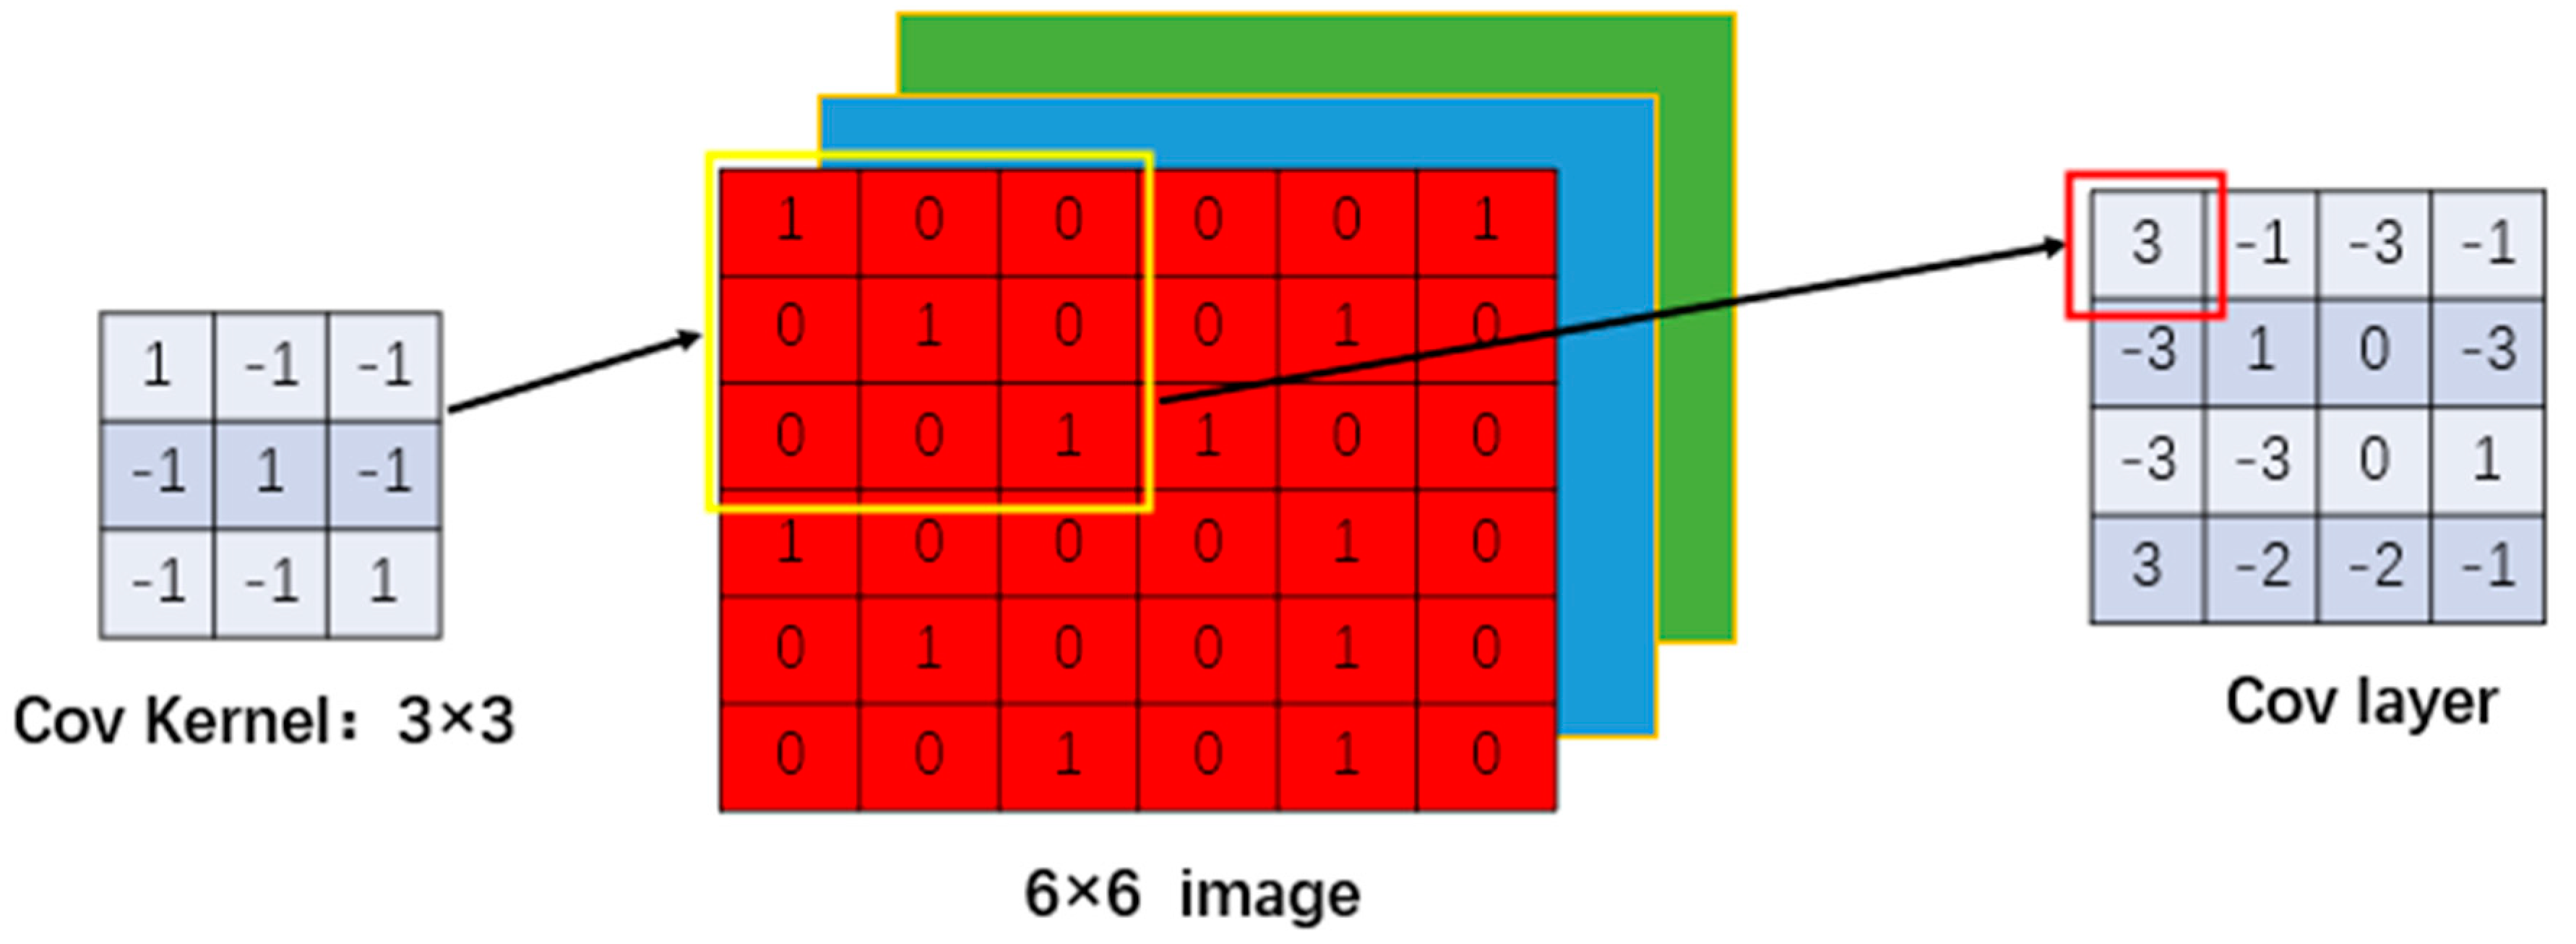
\includegraphics[width=0.60\textwidth]{Images/convlayer.jpg}
  \caption[Example of the convolution process.]{Example of the convolution process. Retrieved from \cite{review:DL}.}
  \label{fig:convlayer}
\end{figure}

Here we can also define the terms stride and padding. Stride is the number of pixels shifts over the input matrix. If the stride is 1, we move the filters by 1 pixel at a time. In Figure \ref{fig:convlayer}, we can see that the size of the output is smaller than that of the input. To keep the dimension of the output equal to the input, padding is used where zeros are symmetrically added to the input matrix \cite{guide:cnn}.

The goal of the convolution operation is to extract high-level features from the input image. The more convolutional layers or the more kernels used in each convolutional layer, the higher the number of features extracted.



\subsubsection*{Pooling Layer}

In most cases, a convolutional layer is followed by a pooling layer. The main goal of this layer is to reduce the size of the convolved feature map in order to reduce the computational costs. This is performed by sliding a two-dimensional filter over each channel of the feature map and summarising the features that lie within the region covered by the filter. There are several types of pooling operations, but the most commonly used is the max pooling which returns the maximum value from the portion of the image covered by the filter \cite{2018guide}.

\subsubsection*{Activation Functions}

One of the main parameters in a \ac{CNN} model is the activation function. This nonlinear function can be interpreted as a selection mechanism that decides whether a particular neuron should fire or not given its input. They are often placed directly after the convolutional layer to introduce non-linearity into the feature map.

There are several commonly used activation functions such as the sigmoid, \ac{Tanh}, \ac{ReLU}, \ac{Leaky ReLU} and \ac{ELU} functions. The most commonly used function in neural networks is \ac{ReLU} (Equation \ref{eq:relu}) because it is very computationally efficient, activating only a few neurons per time, it does not saturate in the positive domain, and it converges faster than the tanh and sigmoid activation functions \cite{2018activation}.

\begin{equation}
    relu(x) = \max{\{0,x\}}
    \label{eq:relu}
\end{equation}

\subsubsection*{Fully Connected Layer}

\ac{FC} Layers usually form the last few layers of the network. The input to the fully connected layer is the output of the last pooling or convolutional layer, which is flattened and then fed into the fully connected layer. The flattened vector then passes through a few more \ac{FC} layers, where the mathematical functions are normally processed. After passing through the fully connected layers, the logistic or softmax activation function is used in the last layer to determine the probability that the input belongs to a certain class (classification) \cite{guide:cnn}. Figure \ref{fig:cnn_class} shows a diagram depicting the basic \ac{CNN} architecture for image classification:

\begin{figure}[!htb]
  \centering
  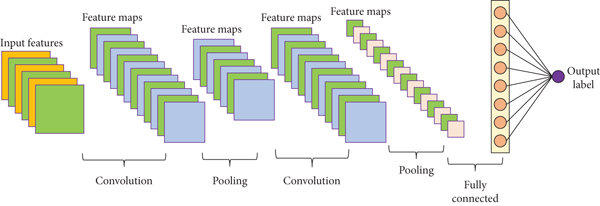
\includegraphics[width=0.75\textwidth]{Images/cnn_class.jpg}
  \caption[Basic \ac{CNN} architecture for image classification.]{Basic \ac{CNN} architecture for image classification. Retrieved from \cite{image:CNN}}
  \label{fig:cnn_class}
\end{figure}

\subsection{CNN architecture for Segmentation}

The \ac{CNN} architecture for segmentation uses encoder and decoder models. The encoders are used to downsample the spatial resolution of the input to develop a lower resolution feature mapping. The decoder then takes this feature representation as input and upsamples it to a full resolution segmentation map. The encoders can be convolutional neural networks and the decoders can be based on the deconvolutional or transposed neural networks with the purpose of creating a segmentation map \cite{enconders}. Figure \ref{fig:cnn_seg} shows the basic \ac{CNN} architecture for image segmentation.

\begin{figure}[!htb]
  \centering
  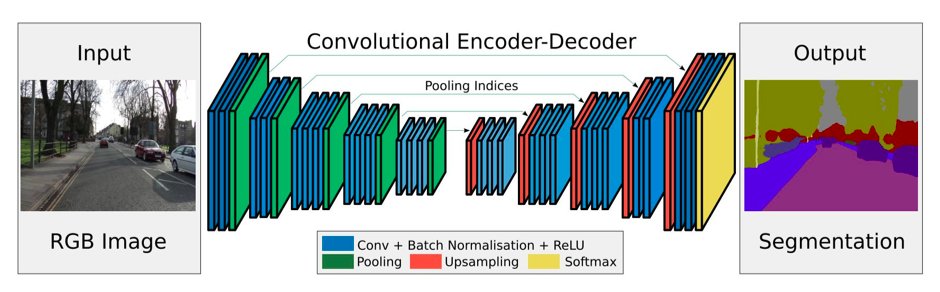
\includegraphics[width=0.75\textwidth]{Images/seg_cnn.jpg}
  \caption[Example of \ac{CNN} architecture for image segmentation.]{Example of \ac{CNN} architecture for image segmentation. Retrieved from \cite{segnet}.}
  \label{fig:cnn_seg}
\end{figure}

\subsection*{\ac{3D} \ac{CNN}}
\label{subsection:3dcnn}
In \ac{3D} \ac{CNN} architectures, the \ac{2D} convolutional and pooling layers are replaced by \ac{3D} convolutional and pooling layers. A \ac{3D} \ac{CNN} can extract more features of the volumes on the three axes X, Y, and Z. Therefore, the use of \ac{3D} information in segmentation enables the full exploitation of spatial information.

The \ac{3D} convolution kernel has one more depth than the \ac{2D} convolution kernel, the fourth dimension continues to correspond to the number of channels of the input image. Like the \ac{2D} convolution operation, a value is obtained by sliding the kernel on the height, width, and number of layers on each channel \cite{2018guide}. In figure \ref{fig:cnn_3D} the process of \ac{3D} \ac{CNN} convolution for multichannels is shown.

\begin{figure}[!htb]
  \centering
  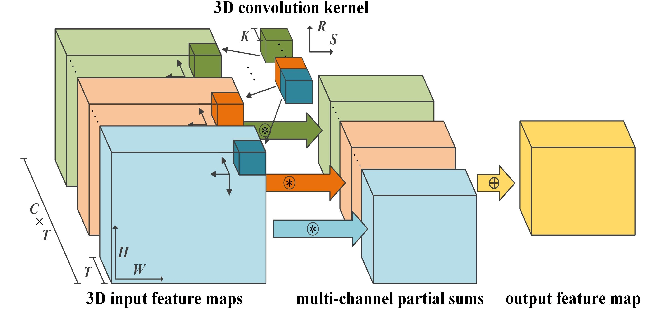
\includegraphics[width=0.65\textwidth]{Images/3dconv.jpg}
  \caption[Illustration of a \ac{3D} convolution layer]{Illustration of a \ac{3D} convolution layer. Retrieved from \cite{CNN:3D}.}
  \label{fig:cnn_3D}
\end{figure}


\subsection{CNN Training}

For training a neural network, the following steps are usually performed:

\begin{itemize}
    \item define the loss function to be minimized during training. For example, in image segmentation tasks, the most commonly used loss function is a pixel-wise cross entropy loss;
    \item select the optimizer that minimizes the loss function by defining how the parameters of the \ac{NN} are updated. The most commonly used optimizers are \ac{SGD}, \ac{SGD} with momentum, \ac{AdaGrad}, \ac{AdaDelta}, RMSProp, and \ac{ADAM}. In these optimizers, the learning rate, which controls how much the model should change in response to the estimated error each time the model weights are updated, is a hyperparameter that must be selected;
    \item split our dataset into a training, validation, and testing dataset. Use the training dataset to adjust the parameters of the model (e.g., the weights and bias in an \ac{NN}), use the validation dataset to test the model with the parameters selected during the training phase, and also use it to stop training when it stops improving (early stopping) and to adjust the hyperparameters. The test data set is used to provide an unbiased evaluation of the final fit of the model to the training data set;
    \item define the maximum number of epochs, one epoch corresponds to one run over the whole training set;
    \item define batch size, the amount of data included in each sub-epoch weight change is called the batch size. Full-batch learning uses all examples of the training set in an epoch, mini-batch learning uses only a subset of the training set, and online learning uses only one example of the training set. For example, for a training set of 100 examples, a full batch size would be 100, a mini-batch size would be 50 or 20 or 10, and an online batch size would be only 1.
    
\end{itemize}

%%%%%%%%%%%%%%%%%%%%%%%%%%%%%% U NET %%%%%%%%%%%%%%%%%%%%%%%%%%%%%%%%%%


\subsection{U-Net}

U-Net is a convolutional neural network developed by \citet{Unet:2D} for biomedical image semantic segmentation. The network is based on the \ac{FCN} \cite{fcn} and its architecture was modified and extended to work with fewer training images and to yield more precise segmentation. 

\subsubsection*{U-Net Architecture}

\begin{figure}[!htb]
  \centering
  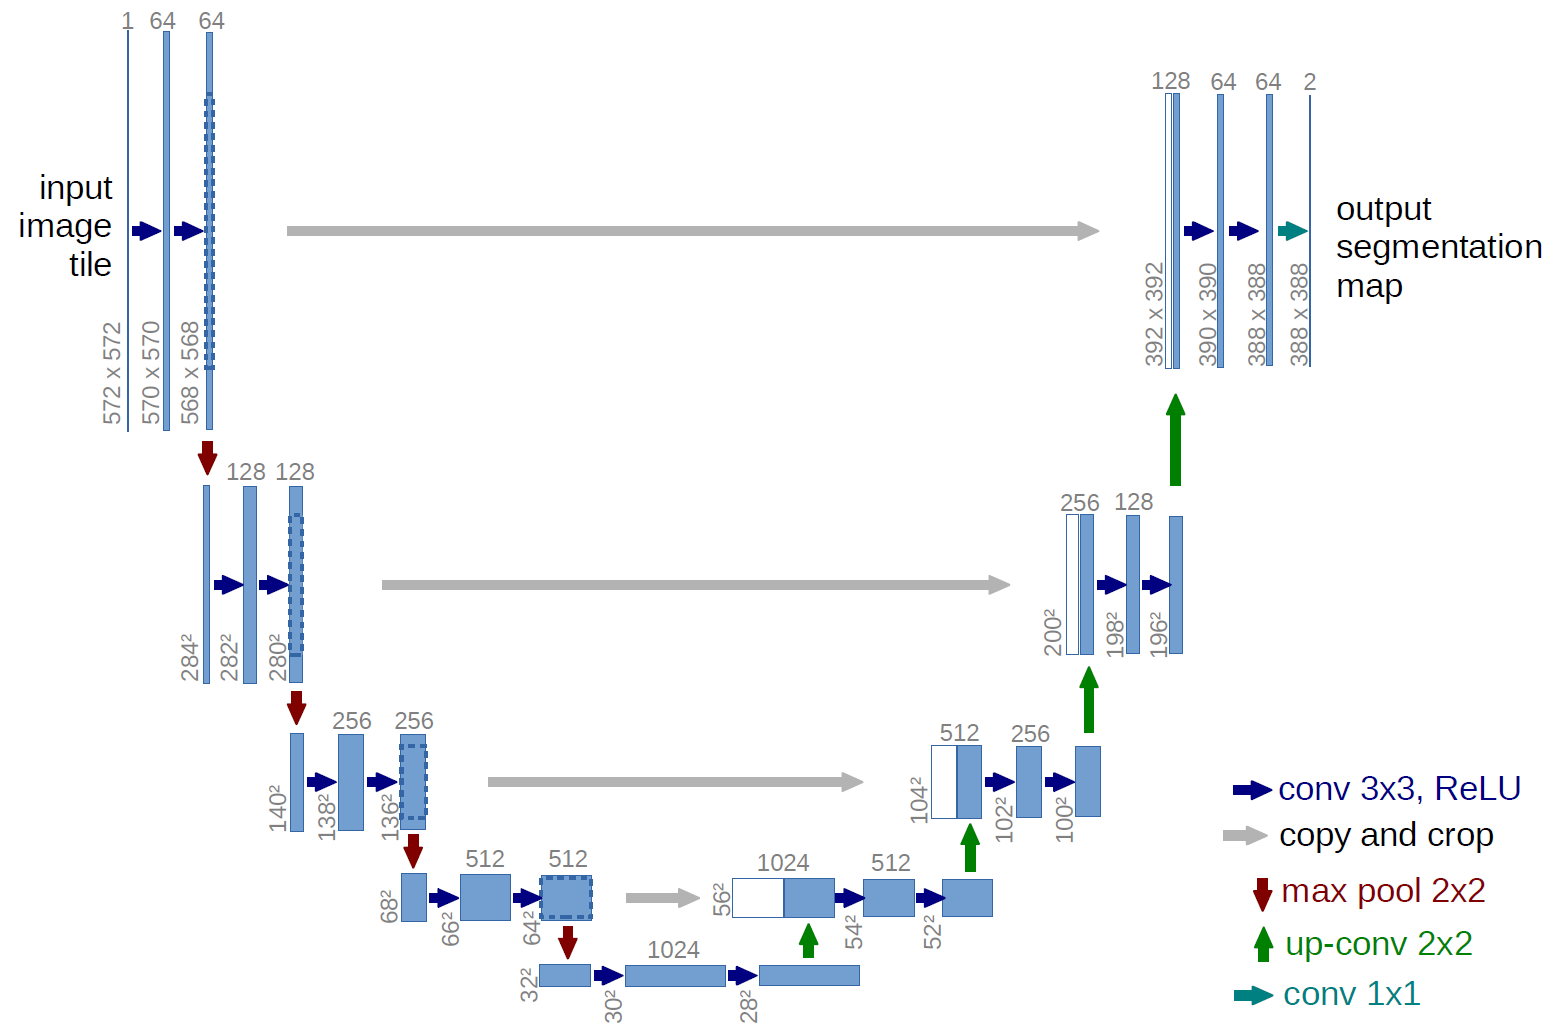
\includegraphics[width=0.85\textwidth]{Images/u-net-architecture.jpg}
  \caption[U-Net architecture.  Each blue box corresponds to a multi-channel feature map. The number of channels is denoted on top of the box. The x-y-size is provided at the lower left edge of the box. White boxes represent copied feature maps. The arrows denote the different operations.]{U-Net architecture. Each blue box corresponds to a multi-channel feature map. The number of channels is denoted on top of the box. The x-y-size is provided at the lower left edge of the box. White boxes represent copied feature maps. The arrows denote the different operations. Retrieved from \cite{Unet:2D}.}
  \label{fig:Unet:2D}
\end{figure}

The U-Net model takes its name from the fact that its architecture is in the shape of a 'U'. This architecture consists of three sections: the contraction (encoder), the bottleneck, and the expansion section (decoder). The encoder follows the typical architecture of a convolutional network. It consists of the repeated application of two unpadded 3x3 convolutions, each followed by a rectified linear unit and a 2x2 max-pooling operation with stride 2 for downsampling. At each downsampling step the number of feature channels is doubled. On this contraction path, the model captures the important features of the image and discards the unimportant ones, reducing the resolution of the image at each convolution+maxpool layer. The bottommost layer (bottleneck) mediates between the contraction layer and the expansion layer. It uses two 3x3 \ac{CNN} layers followed by 2x2 up-convolution layer.

In the expansive path, each step consists of: an upsampling of the feature map, followed by a 2x2 convolutional layer (up-convolution) that reduces the number of feature maps by half to preserve symmetry; a skip-connection and concatenation with the correspondingly cropped feature map from the contracting path, this allows valuable details learned in the encoder part to be used to construct an image in the decoder part; and two 3x3 convolutions, each followed by a \ac{ReLU}. Cropping is necessary because edge pixels are lost with each convolution. In the last layer, a 1x1 convolution is used to assign each 64-component feature vector to the desired number of classes.


\subsubsection*{Loss function}

The loss function is computed by a pixel-wise softmax over the final feature map in combination with the cross-entropy loss function. In addition, the authors introduce a weighting map into the loss function, where each pixel is assigned a weight and pixels on the boundary of segmented objects (cells in this case) have a higher weight. In this way, the network is "forced" to learn the boundary pixels.

\subsection{3D U-Net}
\label{subsection:3dunet}

\citet{Unet:3D} proposed a \ac{3D} U-Net model, as an extension of the original U-Net \cite{Unet:2D}, with the objective of making the U-Net structure have richer spatial information. The network structure is shown in figure \ref{fig:3dUnet}. 

\begin{figure}[!htb]
  \centering
  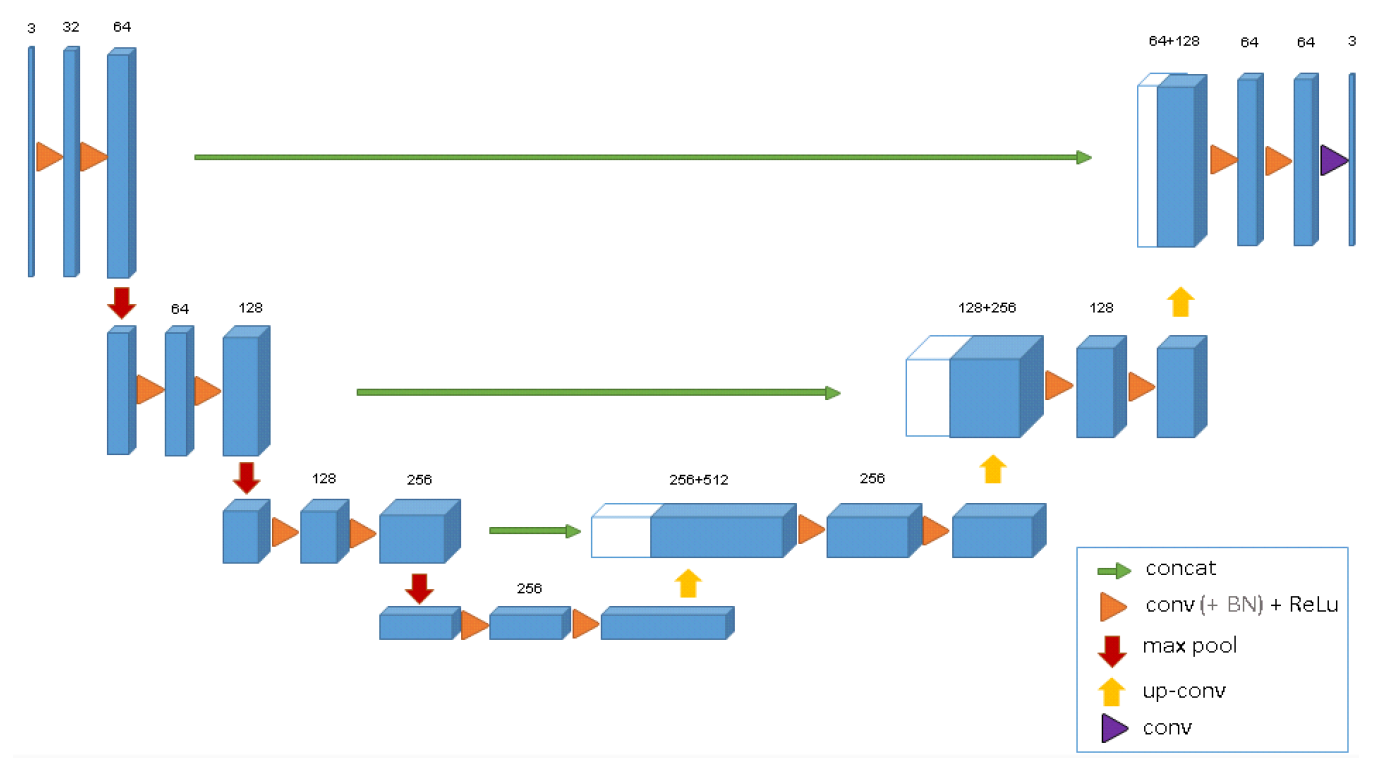
\includegraphics[width=0.85\textwidth]{Images/3dunet.jpg}
  \caption[\ac{3D} U-Net architecture.]{\ac{3D} U-Net architecture. Retrieved from \cite{Unet:3D}.}
  \label{fig:3dUnet}
\end{figure}

Similar to the \ac{2D} U-Net, the \ac{3D} U-Net architecture consists of an analysis path (left) and a synthesis path (right). The main difference is in the size of the kernels applied in the different layers (see subsection \nameref{subsection:3dcnn} for an explanation and illustration of a \ac{3D} convolutional layer). Here 3x3x3 convolutions and up-convolutions and 2x2x2 max-pooling are used, and a 1×1×1 convolution reduces the number of output channels to the number of labels. 

The authors also introduced \ac{BN} before each \ac{ReLU}. Batch normalization is a technique for training deep neural networks, where the inputs for a layer are standardized for each mini-batch. This helps to speed up the training and stabilize the learning process.

In addition, the authors continue to use softmax with weighted cross entropy as the loss function.


\section{Generative Adversarial Networks}
\label{section:GANs}
In 2014, \citet{GAN_original} introduced Generative Adversarial Networks. \ac{GANs} are an approach to generative modeling using deep learning methods, such as convolutional neural networks. Generative models capture, for a given set of data instances X and a set of labels Y, the joint probability $p(X, Y)$. In \ac{GANs}, a generative model is trained to generate realistic samples of the input data on which they have been trained.

More specifically, \ac{GANs} are algorithmic architectures inspired by game theory in which 2 neural networks, a generator and a discriminator, compete to reinforce each other. 

In a \ac{GAN}, the generator (G) is the neural network that learns the underlying distribution of the data. It receives as input a noise variable and outputs a synthetic sample. The discriminator (D) is a binary classifier that receives images as input and outputs the probability that the image is real (i.e., from the actual training set) or fake (i.e., from the generator). In this approach, the generator is trained to capture the distribution of the real data so that its generative samples are as close as possible to the real ones, or in other words, make the discriminator classify them as coming from the real dataset. The architecture of a \ac{GAN} model is shown in Figure \ref{GAN}. 

\begin{figure}[!htb]
  \centering
  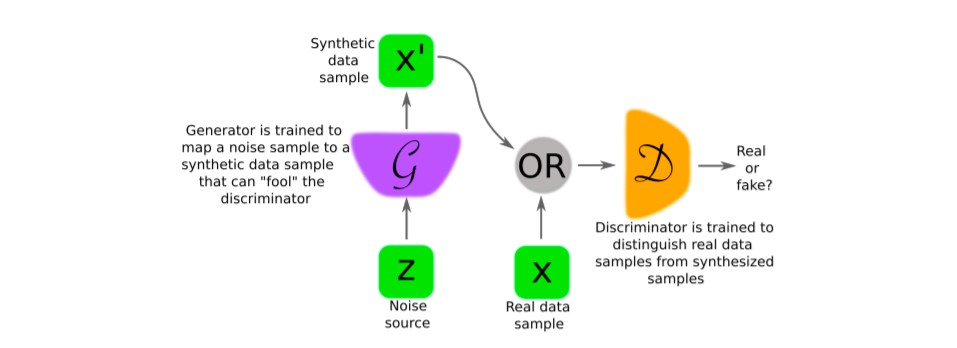
\includegraphics[width=0.90\textwidth]{Images/GAN.jpg}
  \caption[Schematic of the \ac{GAN} model. Where G and D are usually implemented as neural networks.]{Schematic of the \ac{GAN} model. Where G and D are usually implemented as neural networks. Retrieved from \cite{GAN}.}
  \label{GAN}
\end{figure}

\subsection{Training GANs}

The generator and discriminator of \ac{GANs} may have different architectures. However, since \ac{GANs} usually work with image data, they often use \ac{CNNs} as generator and discriminator models.

\subsubsection*{Loss Function}

To train a \ac{GAN}, we first need to define the loss functions of the generator and discriminator. Some notations to keep in mind are:

\begin{itemize}
    \item $p_{data}(x)$: the distribution of real data
    \item $x$: sample from $p_{data}(x)$
    \item $p(z)$: distribution of random input
    \item $z$: sample from $p(z)$
    \item $G(z)$: Generator Network
    \item $D(x)$: Discriminator Network
\end{itemize}

Since the discriminator is a binary classifier, it can be trained using the binary cross entropy loss function. As mentioned earlier, the discriminator aims to maximize the probability assigned to real and fake images. In mathematical terms, the discriminator seeks to maximize the average of the log likelihood for real images and the log value of the inverted likelihoods for fake images. Therefore, the loss function of the discriminator over a batch is given by:

\begin{equation}
    \max [\mathbb{E}_{x\sim p_{data}(x)}[\log{D(x)}]+\mathbb{E}_{z\sim p_{z}(z)}[\log{(1-D(G(z)))}]].
    \label{eq:GAN}
\end{equation}

The generator seeks to minimize the log of the inverse probability predicted by the discriminator for fake images. This has the effect of encouraging the generator to generate samples that have a low probability of being fake. This can be described as the following:

\begin{equation}
    \min [\mathbb{E}_{z\sim p_{z}(z)}[\log{(1-D(G(z)))}]].
\end{equation}

With this, we can write the final loss function as:

\begin{equation}
   \min_{G} \max_{D} [\mathbb{E}_{x\sim p_{data}(x)}[\log{D(x)}]+\mathbb{E}_{z\sim p_{z}(z)}[\log{(1-D(G(z)))}]].
\end{equation}

This means that the discriminator parameters (defined by D) maximize the loss function and the generator parameters (defined by G) minimize the loss function.

\subsubsection*{Training steps} 

The original \ac{GAN} paper provides a pseudo-code that shows how a \ac{GAN} is trained, this is shown in algorithm \ref{alg:GAN}.

\begin{algorithm}
  \scriptsize
  \caption[Minibatch stochastic gradient descent training of generative adversarial networks.]{Minibatch stochastic gradient descent training of generative adversarial networks. Retrieved from \cite{GAN_original}.}\label{alg:GAN}
  \For{number of training iterations}{

    \For{$k$ steps}{
      \begin{itemize}
        \itemsep0em 
        \item Sample minibatch of $m$ noise samples $\left\{\boldsymbol{z}^{(1)}, \ldots, \boldsymbol{z}^{(m)}\right\}$ from noise prior $p_g(\boldsymbol{z})$.
        \item Sample minibatch of $m$ examples $\left\{\boldsymbol{x}^{(1)}, \ldots, \boldsymbol{x}^{(m)}\right\}$ from data generating distribution $p_{\text {data }}(\boldsymbol{x})$.
        \item Update the discriminator by ascending its stochastic gradient:
        $$
        \nabla_{\theta_d} \frac{1}{m} \sum_{i=1}^m\left[\log D\left(\boldsymbol{x}^{(i)}\right)+\log \left(1-D\left(G\left(\boldsymbol{z}^{(i)}\right)\right)\right)\right] .
        $$
      \end{itemize}
    }
  
    \begin{itemize}
      \itemsep0em 
      \item Sample minibatch of $m$ noise samples $\left\{\boldsymbol{z}^{(1)}, \ldots, \boldsymbol{z}^{(m)}\right\}$ from noise prior $p_g(\boldsymbol{z})$.
      \item Update the generator by descending its stochastic gradient:
      $$
      \nabla_{\theta_g} \frac{1}{m} \sum_{i=1}^m \log \left(1-D\left(G\left(z^{(i)}\right)\right)\right) .
      $$
    \end{itemize}
  }
\end{algorithm}


In the algorithm \ref{alg:GAN} it's evident that the \ac{GAN} training proceeds in alternating periods:

\begin{enumerate}
  \item The discriminator trains for $k$ steps ($k$=1 in \cite{GAN_original}), and during this period the generator is not trained;
  \item The generator is updated only after $k$ steps, and during this period the discriminator is not trained; 
  \item Repeat steps 1 and 2, for a specified number of iterations, to further train the generator and discriminator networks.
\end{enumerate}

\subsection{Supervised GAN example: Pix2Pix}
\label{subsection:pix2pix}

In recent years, several \ac{GAN} models have been proposed to perform different tasks. One of these models is Pix2Pix, which was introduced by \citet{isola2018imagetoimage} to accomplish the task of image-to-image translation.

Pix2Pix is an implementation of the \ac{cGAN}, where the generation of an image depends on another given image. The general architecture of a \ac{cGAN} model is shown in Figure \ref{fig:cGAN}.

\begin{figure}[!htb]
  \centering
  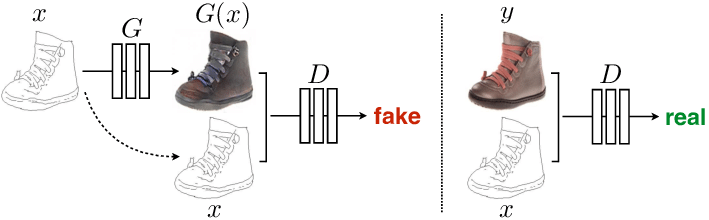
\includegraphics[width=0.70\textwidth]{Images/Training-a-conditional-GAN-to-map-edgesphoto-The-discriminator-D-learns-to-classify.jpg}
  \caption[Schematic of the \ac{cGAN} model.]{Schematic of the \ac{cGAN} model. Retrieved from \cite{isola2018imagetoimage}.}
  \label{fig:cGAN}
\end{figure}


As shown in Figure \ref{fig:cGAN}, the generator model receives a given image as input and generates a translated version of the image. The discriminator model receives an input image from the source domain and an image from the target domain and must determine whether the image from the target domain is a real or generated version of the source image. Finally, the generator model is trained to both fool the discriminator model and minimize the loss between the generated image and the expected target image. Therefore, the Pix2Pix \ac{GAN} must be trained on image datasets consisting of input images (before translation) and output or target images (after translation).


\subsubsection*{Generator and discriminator architecture}

In \cite{isola2018imagetoimage}, a U-Net model is used for the generator, and, after well trained, it takes as input an image from the source domain and outputs an image in the target domain. 

For the discriminator, the authors chose the PatchGAN discriminator. The PatchGAN, also called the Markov discriminator, classifies individual (N x N) patches in the image as real or fake, rather than classifying the entire image as real or fake. The output of the network is a single feature map of real/fake predictions that can be averaged to give a single classification score. The advantage of using a PatchGAN over a normal \ac{GAN} discriminator is that it has fewer parameters than a normal discriminator and can work with images of any size.

\subsubsection*{Loss Function}

The conditional adversarial Loss is defined as follows:

\begin{equation}
    \mathcal{L}_{cGAN}(G,D) = \mathbb{E}_{x,y} [\log{D(x,y)}] + \mathbb{E}_{x,z} [\log{(1-D(x,G(x,z)))}],
    \label{eq:1}
\end{equation}

where $x$ is the input observed image, $y$ is the real target image, $z$ is a random noise vector and $G(x,z)$ is the output generated image.

The generator model is trained using both the adversarial loss for the discriminator model and the $L_1$ or mean absolute pixel difference between the generated translation of the source image and the expected target image. The adversarial loss affects whether the generator model can output images that are plausible in the target domain, while the $L_1$ loss regularizes the generator model to output images that are plausible translations of the source image.

The L1 loss function is shown below:

\begin{equation}
    \mathcal{L}_{1}(G) = \mathbb{E}_{x,y,z} [||y-G(x,z)||_1].
    \label{eq:2}
\end{equation}

Combining these functions from \ref{eq:1} and \ref{eq:2}, results in the final objective function:

\begin{equation}
    G^* = \arg \min_{G}\max_{D} \mathcal{L}_{cGAN}(G,D) + \lambda_1  \mathcal{L}_{1}(G)
\end{equation}

where $\lambda_1$ is a hyperparameter that controls the relative importance of the L1 loss term. 

\subsection{Unsupervised GAN example: CycleGAN}
\label{subsection:CycleGAN}

As shown, the Pix2Pix model is capable of solving the image-to-image translation problem, but only if we have a paired training dataset available, i.e., a large dataset with many examples of input images X and the same image with the desired change that can be used as the expected output image Y. However, obtaining this training data is difficult in many cases. 

In 2017, \citet{cycleGAN:original} proposed a novel approach to address the unpaired image-to-image translation problem, called CycleGAN, which uses a \ac{GAN} architecture. 

As can be seen in Figure \ref{fig:cyclegan}, CycleGAN consists of two generator models, one generator (Generator 1) synthesizes images for the domain X to domain Y and the other generator (Generator 2) synthesizes images for the domain Y to domain X. Each generator has a corresponding discriminator model (Discriminator 1 and Discriminator 2). The discriminator model (1/2) takes real images from domain (Y/X) and generated images from the Generator (1/2) and predicts whether they are real or fake. 

\begin{figure}[!htb]
  \centering
  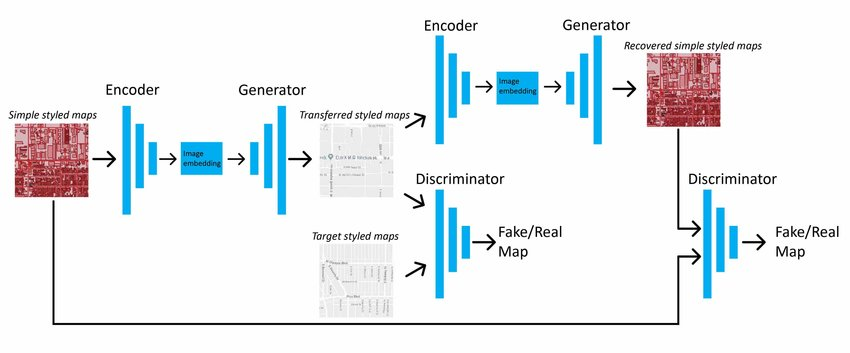
\includegraphics[width=0.90\textwidth]{Images/Data-flow-of-CycleGAN-in-this-research.jpg}
  \caption[Example of schematic of the CycleGAN model.]{Example of schematic of the CycleGAN model. Retrieved from \cite{cyclegan:image}.}
  \label{fig:cyclegan}
\end{figure}

\subsubsection*{Loss function}

The loss function used to train the generators consists of three parts: adversarial loss, cycle consistency, and identity loss. The adversarial loss  is applied to both generators. For the first \ac{GAN} (generator 1, discriminator 1), the adversarial loss is expressed as follows:

\begin{equation} \mathcal{L}_{ GAN }(G_1,D_1,X,Y)=\mathbb{E}_{y\sim p_{data}(y)}[\log{D_1(y)}]+\mathbb{E}_{x\sim p_{data}(x)}[\log{(1-D_1(G_1(x)))}]. 
\end{equation} 

For the second \ac{GAN} (generator 2, discriminator 2) is expressed as:

\begin{equation} \mathcal{L}_{ GAN }(G_2,D_2,Y,X)=\mathbb{E}_{x\sim p_{data}(x)}[\log{D_2(x)}]+\mathbb{E}_{y\sim p_{data}(y)}[\log{(1-D_2(G(y)))}]. 
\end{equation}
 
As in the original \ac{GAN} model, the generators try to minimize these losses, while the respective discriminators try to maximize them. Cycle consistency loss is a new term introduced to ensure that we preserve the original image when translating it from one domain to another and back again. Therefore, it calculates the $L_1$ loss between the original image and the generated one in two directions: $x \rightarrow G_1(x) \rightarrow G_2(G_1(x)) \approx x$ and $y \rightarrow G_2(y) \rightarrow G_1(G_2(y)) \approx y$. The cycle consistency loss is expressed as follows:

\begin{equation} 
\mathcal{L}_{cyc} = \mathbb{E}_{x\sim p_{data}(x)} [||G_{2}(G_{1}(x))-x||_1] + \mathbb{E}_{y\sim p_{data}(y)} [||G_{1}(G_{2}(y))-y||_1].
\label{eq:CCL}
\end{equation}

Finally, the identity loss is an additional optional term used mainly to preserve the color composition between input and output. It is computed by giving the generator an image of its target domain as input and computing the $L_1$ loss between input and the generated images. This loss is expressed as follows:

\begin{equation} 
\mathcal{L}_{id}(G_1,G_2) = \mathbb{E}_{y\sim p_{data}(y)} [||G_{1}(y)-y||_1] + \mathbb{E}_{x\sim p_{data}(x)} [||G_{2}(x)-x||_1].
\label{eq:identity}
\end{equation}

\section{Metrics to evaluate semantic segmentation models}

Various metrics are used to validate and test the performance of these segmentation models, the most important of which are described below.

\textbf{Pixel Accuracy} is the percentage of pixels in the image that were correctly classified. Here, a true positive/false positive (TP/FP) value represents a pixel that was correctly/incorrectly predicted as belonging to a particular class (according to the target mask), while a true negative/false negative (TN/FN) value represents a pixel that was correctly/incorrectly predicted as not belonging to a particular class.

\begin{equation}
    Accuracy = \frac{TP+TN}{TP+TN+FP+FN}
\end{equation}

\textbf{Precision} describes the \textit{purity} of positive predictions with respect to ground truth, i.e., it measures, of all the pixels predicted in a given image, how many of those pixels actually match with ground truth.

\begin{equation}
    Precision = \frac{TP}{TP+FP}
\end{equation}

\textbf{Recall} describes the \textit{completeness} of positive predictions with respect to the ground truth, i.e., of all pixels annotated in the ground truth, it measures how many of these pixels were capture as positive predictions.

\begin{equation}
    Recall = \frac{TP}{TP+FN}
\end{equation}

\textbf{\ac{IoU}} measures the similarity between two images in semantic segmentation by computing the ratio between the overlapped area and the combined area of prediction and ground truth.

\begin{equation}
    IoU = \frac{TP}{TP+FP+FN}
\end{equation}

\textbf{\ac{DC} (F1 Score)} is also used to measure the similarity between two images. It is equal to two times the overlap area between prediction and ground truth divided by the total number of pixels in both images.

\begin{equation}
    DICE = \frac{2 \ TP}{2 \ TP+FP+FN}
\end{equation}

% Escrever sobre as métricas
% https://towardsdatascience.com/metrics-to-evaluate-your-semantic-segmentation-model-6bcb99639aa2

% If Printing on DOUBLE SIDED pages, the second page should be white.
% Otherwise, comment the following command:
\cleardoublepage
%
%Chapter 3
% #############################################################################
% This is Chapter 3
% !TEX root = ../main.tex
% #############################################################################
% Change the Name of the Chapter i the following line
\fancychapter{State-of-the-Art on Microscopy Image Segmentation}
\cleardoublepage
% The following line allows to ref this chapter
\label{chapter:state_of_the_art}

Fluorescence microscopy has recently become an important tool for the study of cells, as it allows the acquisition and visualization of \ac{3D} image volumes that extend deeper into the tissue. Therefore, as mentioned in section \ref{section:motivation}, automated \ac{3D} microscopy image analysis techniques, specially to perform segmentation, are needed to efficiently and accurately quantify and characterize cells, nuclei, or other biological structures. In this section, we review the current state-of-the-art in microscopic image segmentation (with a particular focus on fluorescence microscopy).


\section{Microscopic image segmentation challenges}

Segmentation of subcellular structures in microscopic images presents many challenges. In particular, during image acquisition, microscopic images often exhibit digital noise, background clutter, and blurring \cite{review:robust}. These problems are exacerbated for microscopic volumes because they are inherently anisotropic and anomalies vary along different axes. As a result, these images often exhibit the following: intensity inhomogeneity, low contrast, limited depth resolution, and consequently the subcellular structures being segmented typically have poorly defined edges \cite{active:inhmo}. 

When segmenting nuclei/cells, the challenge becomes even greater because the size, shape, and intracellular intensity heterogeneity of nuclei/cells vary widely and they are often grouped together in clumps so that they sometimes touch and/or overlap \cite{review:robust}. In recent decades, several automated segmentation methods for microscopic images have been investigated that aim to overcome some or all of these challenges.

%\subsection{Preprocessing Techniques}

\section{Classical approaches}
\label{subsection:clas}


In recent years, several classical image processing algorithms have been investigated. In particular, \ac{ACMs} have been widely used in microscopy image segmentation (with a particular focus on fluorescence microscopy) due to their ability to segment structures with different shapes. \ac{ACMs} iteratively minimize an energy/cost function while deforming an initial contour to fit objects of interest. There are several variants of active contours. One is edge-based \ac{ACM}, which uses image gradient maps in object identification \cite{snakes:active}. However, these approaches are sensitive to image noise and depend heavily on the placement of the initial contour. Active contours have also been integrated with region-based approaches, which aim to find an energy balance between foreground and background regions \cite{region:based}. Region-based methods generally achieve better results than edge-based active contours because they are relatively independent of initial contour generation and robust to noise. 


In \cite{3D:active}, a \ac{3D} active surface method is proposed as an extension of the region-based \ac{2D} active contour model of Chan-Vese presented in \cite{region:based} to segment \ac{3D} cell structures of a rat kidney. In \cite{active:inhmo}, a method for segmenting cell nuclei in \ac{3D} microscopy volumes based on a combination of \ac{3D} region-based active contours and \ac{3D} inhomogeneity correction was described. A dataset containing \ac{3D} volumes of cell structures from a rat kidney was used. This method achieved an accuracy of 89.6\%, outperforming the previous method \cite{region:based}. Another well-known biomedical imaging tool is Squassh \cite{squass:original,squassh}, which minimizes an energy function derived from a generalized linear model to segment and quantify \ac{2D} or \ac{3D} subcellular structures. The main problem with these methods is that they are unable to separate overlapping nuclei, which degrades the quality of the segmentation results. 

To separate overlapping cells/nuclei and improve segmentation, several methods have been described. In \cite{active:couple}, a model based on coupled active surfaces for cell segmentation is presented. This framework uses multiple active surfaces coupled by a penalty for overlap and a volume conservation constraint that improves the contouring of cell boundaries \cite{couple:original}. \citet{active:couple} improved this technique, first presented in \cite{couple:original}, by incorporating watershed techniques, a \ac{non-PDE}-based energy minimization, and the Radon transform to improve the separation of touching cells. The evaluation of this method was performed in \ac{3D} time-lapse fluorescence microscopy image datasets of HeLa cells and achieved an average precision of 98.98\%. Moreover, this approach proved to be computationally much more efficient (up to nine times faster) compared to \cite{couple:original}. In \cite{graphs}, Arslan et al. proposed an alternative, a new model-based nuclei segmentation algorithm that defines primitives to represent the boundaries of the nucleus and region growing to delineate the nucleus borders. The model was evaluated on two challenging datasets of fluorescence microscopy images of human hepatocellular carcinoma cell lines and achieved an average precision of 72\%. The experiments in this work show that it leads to better results on overlayed nuclei and is less susceptible to noise.

However, these methods require manual optimization of parameters, are difficult to generalize to different datasets, and are unable to discriminate between different cellular structures. 
 
\section{Convolutional Neural Networks}

Recently, deep learning-based models have gained recognition due to their ability to automatically learn important features from data. In the last decades they have been successfully applied to computer vision tasks, including microscopy image analysis, for nuclei detection, cell segmentation, tissue segmentation, image classification, and so on. Many of them were able to outperform the classical approaches mention in section \ref{subsection:clas} \cite{review_cnn}.

\subsection{Supervised models}

One popular deep architecture is the \ac{CNN} which, given images and corresponding annotations (ground-truth), is able to learn the essential features of an image that are invariant to irrelevant variations \cite{guide:cnn}. \ac{CNNs} have already been successfully implemented in various computer vision tasks, including microscopy segmentation.

In \cite{CNN2}, Xing et al. implemented an automatic nuclei segmentation method using a \ac{CNN}, for nuclei detection, together with a selection-based sparse shape model. The proposed method was able to achieve superior performance, when compared with other classical models, across three different datasets. In \cite{CNN3}, a \ac{CNN} is used to produce a ternary map, contrary to the binary map proposed in \cite{CNN2}. The additional third class is used to identify pixels on the nuclear boundaries, which helps in the segmentation of crowded and sparse nuclei. Another contribution of this paper include the release of a new dataset, MultiOrgan dataset, with a diversity of nuclear appearances from seven organs and a new evaluation metric to better measure the performance of a nuclear segmentation method called \ac{AJI}. The approach obtained reasonable results for different datasets, which shows its generatization hability, and an overall \ac{AJI} of 0.508 and F1-Score of  0.827, outperforming \cite{CNN2} and other open source softwares \cite{cellprofiler}. 

Though these techniques produce good results in \ac{2D} images, they're not applicabe for segmentation of \ac{3D} microscopic image volumes, because they cannot utilize the depth information in a volume. In \cite{Unet:3D}, Çiçek et al. successfully segmented volumetric microscopic images of the Xenopus kidney with a \ac{3D} U-net, by expanding the previous \ac{2D} U-net \cite{Unet:2D} architecture. A more detailed description of the model was presented in subsection \ref{subsection:3dunet}. The metric used to evaluate the model was \ac{IoU}, and the results for the \ac{3D} U-Net yielded an average value of 0.704 compared to the \ac{2D} U-Net which yielded an average \ac{IoU} value of 0.547. However, the results of the experiments also show that the performance of the network is highly dependent on the amount of annotated data available, as it performed better in semi-automatic segmentation than in fully automatic segmentation.

% https://towardsdatascience.com/review-3d-u-net-volumetric-segmentation-medical-image-segmentation-8b592560fac1 - caso queiras completar

Supervised deep neural network methods, like the ones mentioned above, require a large amount of pixel-wise annotated data for training. Obtaining these detailed annotations is not only time consuming, especially for \ac{3D} volumes, but also must be done by an expert. Therefore, the interest in weakly/fully unsupervised deep learning models that perform well on data without annotation has increased significantly in recent years.

\subsection{Weakly Supervised / Unsupervised models}

In \cite{weakly:2D} and \cite{weakly:3D}, weakly supervised methods were successfully used to segment cell nuclei in \ac{2D} and \ac{3D} microscopy images, respectively. \citet{weakly:2D} proposed the use of points annotation for nuclei segmentation. From these annotations, two types of coarse labels are derived using the Voronoi diagram and the k-means clustering algorithm. These labels are then used to train a \ac{CNN} with cross-entropy loss. The authors also implement a dense CRF loss to refine the trained model. The performance of the model was evaluated using the MultiOrgan dataset of \cite{CNN3}, for which an accuracy of 0.907 and an \ac{AJI} value of 0.510 were obtained. It has been shown that the performance of the weakly supervised method is close to the fully supervised models with the same network structure and, moreover, the annotation time spent on each image is greatly reduced. However, from the \ac{AJI} value, we can also conclude that the nuclear shapes and separation can still be improved.

In \cite{weakly:3D}, a model for segmenting \ac{3D} instances is proposed that uses weak annotations for training. Detection of all instances of interest is achieved using \ac{3D} bounding boxes, and segmentation is achieved for all detected instances by using the full voxel annotation only for a small subset of the instances. For segmentation, the authors use a Fully Convolutional Network backbone with VoxRes block \cite{voxresnet}. The performance of the detection model is compared with the supervised method VoxResNet \cite{voxresnet} and it was found to achieve similar performance with less annotation time. However, the annotation time is still very long (at least 5.5 hours).

Although these methods help to minimize the amount of work required to label images, approaches have been presented in the literature that allow for completely unsupervised segmentation of medical images. \citet{SOTA:3DCNN} proposed an unsupervised approach to segment cell nuclei from \ac{3D} fluorescence microscopy images. For this purpose, a \ac{3D} \ac{CNN} with an encoder-decoder struture was constructed and trained with generated synthetic microscopy volumes and synthetic ground truth volumes containing multiple cell nuclei. The performance of the model was compared with the previously discussed active surface models \cite{3D:active,active:inhmo}, Squassh \cite{squassh}, and a \ac{2D} \ac{CNN} model \cite{2dplus}, and it achieved better results than the first two and similar results to the \ac{2D} \ac{CNN}, with an accuracy of 92.93\%. However, the false detection rate is higher than the best results, i.e., the model tends to over-segment. In \cite{3d:detection} the authors present a method, based on \cite{SOTA:3DCNN}, for detection and segmentation of cell nuclei in \ac{3D} fluorescence microscopy images. In this approach, each nuclear center is detected using adaptive \ac{3D} histogram equalization, \ac{3D} distance transformation, and \ac{3D} classification \ac{CNN}. Then, the nuclei surrounding the seeds are segmented using a \ac{3D} segmentation \ac{CNN}. This approach has been shown to perform better than \cite{SOTA:3DCNN}, but is unable to detect all the nuclei, resulting in under-segmentation (high false negative rate). 

\section{Generative Adversarial Networks}

The performance of \ac{CNN} architectures is always limited by the quantity and quality of the dataset used for training. This is where the \ac{GAN} model comes into play to significantly improve the performance of these approaches due to their superior ability to generate data as well as translate it, as mentioned in section \ref{section:GANs}.

\subsection{Supervised models}

In \cite{cCGAN}, a robust transfer learning framework for the segmentation of HEp-2 Specimen image segmentation using \ac{GAN} is presented. A novel conditional generative adversarial network with classifier (cC- GAN) is introduced to solve the overfitting problem of most DL models by improving their transfer capacity. Using this method, a segmentation accuracy of 75.27\% was achieved in the MIVIA dataset, showing the great potential of applying \ac{GAN} models to microscopic segmentation problems.

\subsection{Weakly Supervised / Unsupervised models}

In \cite{weakly:GAN}, a weakly supervised approach to nucleus segmentation is proposed. A point labelling is used as a weak labelling, then the author uses a Pix2Pix network model to detect the centroid of the nucleus and build a likelihood map, a guided propagation to build a pixel contribution map of the nucleus, and a graph cut to obtain the final instance segmentation. The proposed approach is able to outperform the fully supervised U-Net \cite{Unet:2D} model.

In a multi-organ study for nuclei segmentation on histopathology images \cite{cGAN:cycleGAN}, the authors used CycleGAN and \ac{cGAN} models. First, a CycleGAN model was trained with images from four different organs to synthetically generate pathology data along with perfectly segmented nuclei labels. The real and synthetically generated images were then used to train a \ac{cGAN} to perform nuclei segmentation. This segmentation network showed a 29.19\% improvement in \ac{AJI} compared to the previously mentioned supervised model \ac{CNN}-3C \cite{CNN3} and of 73.19\% compared to the U-Net model \cite{Unet:2D}.


The work proposed in \cite{SOTA:3DCNN} was improved in \cite{3D:CycleGAN} by integrating \ac{GAN}. A challenging problem in previous work has been the difficulty in generating realistic synthetic microscopic data to train the \ac{CNN}, due to the natural diversity of biological structures. \citet{3D:CycleGAN} addressed this problem with a modified model of CycleGAN, a spatially constrained CycleGAN, SpCycleGAN. The spatially constrained CycleGAN is used to generate \ac{3D} realistic synthetic training data. Then, a modified \ac{3D} U-Net network is trained with these \ac{3D} synthetic data to segment nuclei structures. The final accuracy result was 94.59\%, outperforming \cite{SOTA:3DCNN}. However, because this model has some difficulty separating cell nuclei, an extension of this approach for nuclei detection and segmentation was presented in \cite{detection:3D}, using the synthetically generated images from SpCycleGAN to train a \ac{CNN} architecture for classification and segmentation.

DeepSynth \cite{deepsynth} is currently recognized as the state-of-the-art deep model for unsupervised \ac{3D} nuclei segmentation, and is based on the previously referenced work \cite{2dplus,SOTA:3DCNN,3D:CycleGAN}.

More recently, in 2021, \cite{adgan} treats the segmentation of cell nuclei as an image-to-image translation problem. \citet{adgan} propose a novel end-to-end unsupervised framework called \ac{AD-GAN}. They performed segmentation of cell nuclei in challenging \ac{2D} and \ac{3D} datasets of microscopic images. This work addresses the problem of lossy transformation \cite{lossy:cyclegan}, which is defined by the content inconsistency between the original images and the corresponding segmentation masks obtained by the model. These inconsistencies include: the deletion/addition of nuclei at the macro level, shape differences at the micro level, and a location offset. With this new and unsupervised model of \ac{GAN}, the authors were able to mitigate the problem of lossy transformations at the macro and micro levels and even extend this work to instance segmentation. The results obtained for the \ac{3D} fluorescence image dataset Scaffold \cite{dataset} were a \ac{DC} of 89\%. This is significantly higher than the compared models, the DeepSynth model \cite{deepsynth} (45.8\%) and other well-known biomedical imaging tools such as Cell-Profiler 3.0 \cite{cellprofiler} (53.1\%) and Squassh (62.3\%) \cite{squassh}.

In summary, several approaches have been proposed for the segmentation of subcellular structures in microscopic images, and some of the best results have been obtained with deep learning-based models. These models can be trained in a supervised or weakly/unsupervised manner. The advantage of unsupervised models is their independence from annotated data for training. State-of-the-art unsupervised approach presented in \cite{deepsynth} used the CycleGAN as a two-stage pipeline to train a robust segmentor with CycleGAN-synthesized data. However, this adds time and computational costs and significantly increases the complexity of the system. In this work, it will be implemented a different approach, more similar to the \ac{AD-GAN} model, train an unsupervised end-to-end CycleGAN model to segment subcellular strutures, nuclei and Golgi, in fluorescence microscopy images.


%state-of-the-art model  use CycleGAN as a twodeveloped are a two-stage pipeline trying to train a robust segmentor with a two-stage pipeline. The proposed model will try to do segmentation of subcellular strutures, nuclei and golgi, with an end-to-end unsupervised model using directly the CycleGAN model to segment the 

%This would introduce extra time and computation cost, and significantly increase the system complexity

%Despite their success, these CycleGAN based methods are usually not trained end-to-end when used in nuclei cell segmentation, since the masks generated by the corresponding generator may contain too many errors. Instead, these methods often engage a two-stage pipeline trying to train a robust segmentor with the potentially erroneous CycleGAN-synthesized data.

% Completar 
% If Printing on DOUBLE SIDED pages, the second page should be white.
% Otherwise, comment the following command:
\cleardoublepage
%
%Chapter 4
% #############################################################################
% This is Chapter 4
% !TEX root = ../main.tex
% #############################################################################
% Change the Name of the Chapter i the following line
\fancychapter{Methodology}
%\cleardoublepage
% The following line allows to ref this chapter
\label{chapter:methodology}

As mentioned earlier, in this work \ac{DL} methods are used to segment fluorescent microscopic images. The first phase is to implement supervised models to accomplish this task of segmenting the nuclei and Golgi of these images. Then we focus on the main goal, which is to implement an unsupervised model that can perform the same task as well or better than the supervised models. And finally, we add a third class to detect the nucleus-Golgi pairs.

This chapter begins by presenting the dataset used to train, validate, and test these models. The proposed approach to semantic segmentation using an unsupervised model is described in Section \ref{section:proposed}. The performance of this approach is compared to the supervised models, which are described in detail in Section \ref{section:comparison}. Then, Section \ref{section:models_inference} describes how the models are used for inference after training. Finally, Section \ref{section:execution_time} describes how the training and testing time of the models is determined to be used as a measure of the performance of the different approaches.

\section{Dataset}
\label{section:dataset}

The dataset used in this work consists of eight crops extracted from \ac{3D} fluorescence microscopy images of mouse retinas. These crops range in size from 257x505x55 to 627x818x61. In these crops, the nuclei are labeled with green fluorescent protein (GFP) and the Golgi are labeled with mCherry. In addition, manually labeled segmentation masks are used for training the proposed supervised methods and evaluating their performance. These masks are RGB, with the red channel containing the segmentation mask of the Golgi and the green channel containing the segmentation mask of the nuclei. The blue channel contains the segmentation mask of the nucleus-Golgi pairs, but only for the task of the 3-class segmentation problem. In this case, the input images and the output masks have 3 channels. For the 2-class segmentation problem, the blue channel is not considered, so the input images and the output masks have only two channels (these masks are converted to RGB for visualization but the blue channel is all zeros).

An example of a \ac{3D} crop and its corresponding manually labelled segmentation masks for the 2-class task and 3-class task can be found in Figure \ref{fig:dataset_original}.

\begin{figure}[!htb]
	\centering
	\subfigure[]{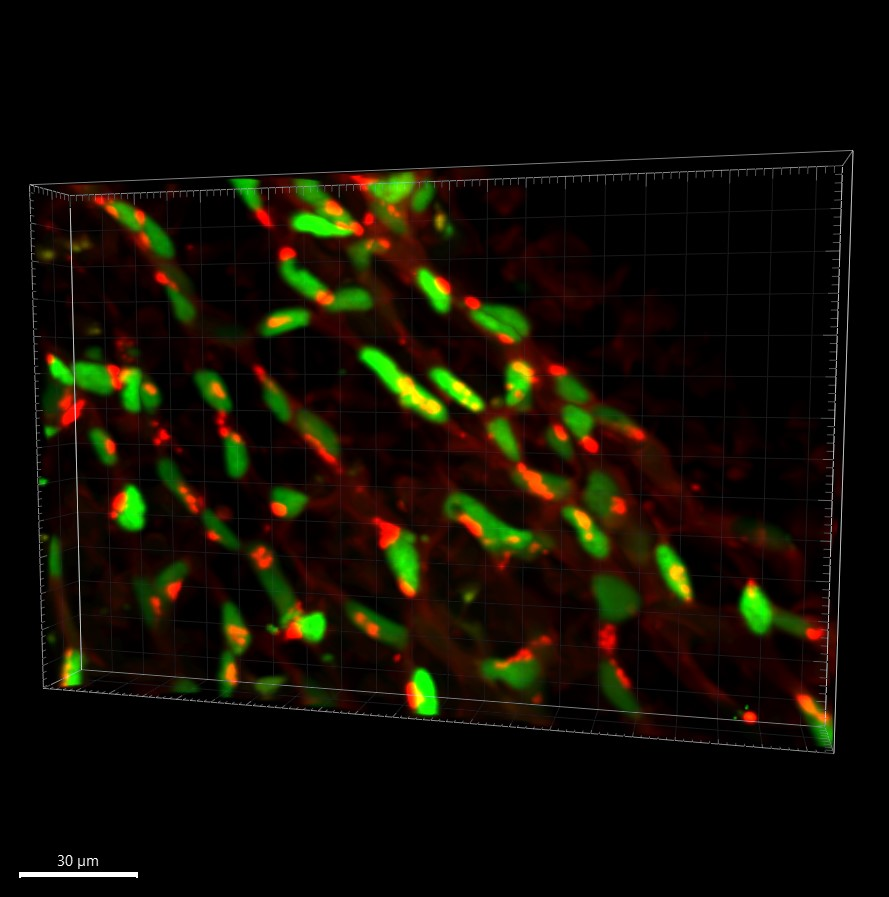
\includegraphics[width=4.5cm]{Images/img_crop1.jpg}}\hfil
  \subfigure[]{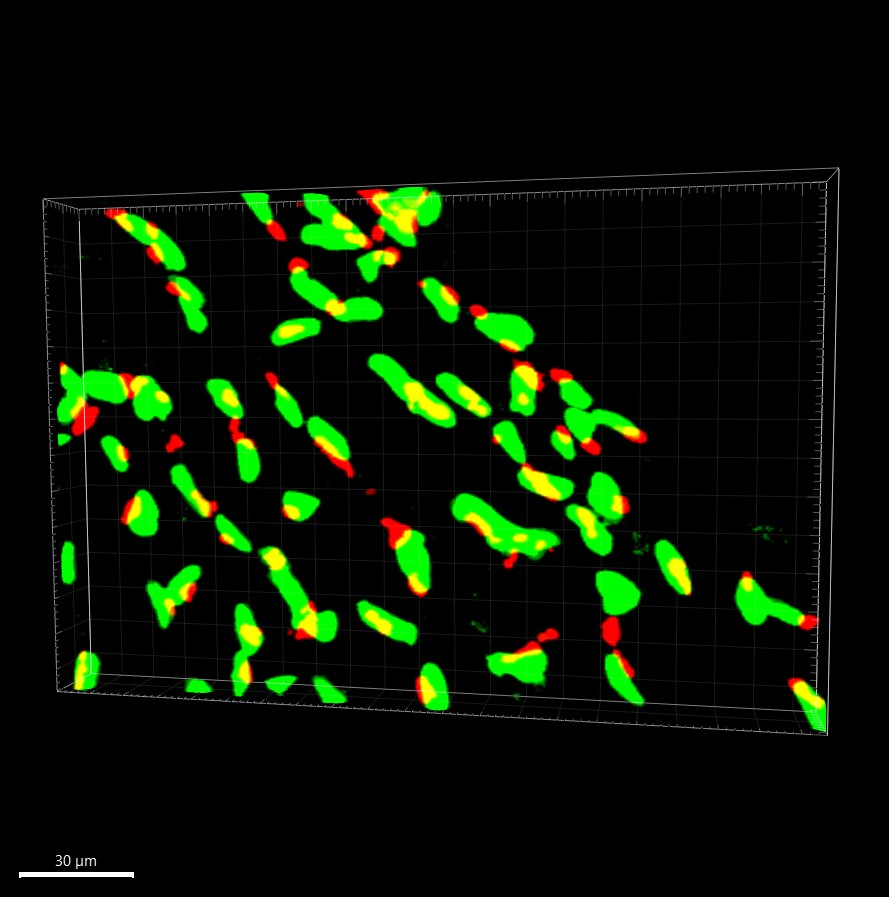
\includegraphics[width=4.5cm]{Images/mask2_crop1.jpg}}\hfil 
  \subfigure[]{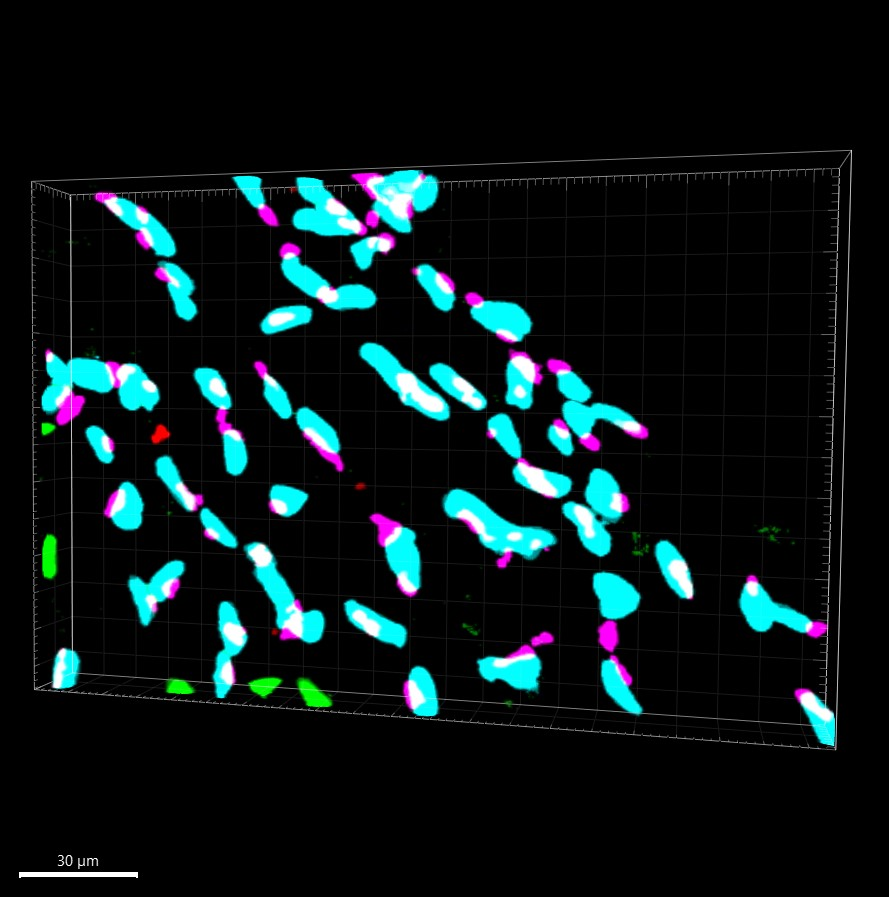
\includegraphics[width=4.5cm]{Images/mask3_crop1.jpg}} 
	\caption[(a) Example of a 3D crop of a microscopy image of mouse retina; (b) 3D ground truth mask for 2-class task; (c) 3D ground truth mask for 3-class task.]{(a) Example of a \ac{3D} crop of a microscopy image of mouse retina; (b) \ac{3D} ground truth mask for 2-class task; (c) \ac{3D} ground truth mask for 3-class task.}
	\label{fig:dataset_original}
\end{figure}

To use these crops to train the models, its necessary to divide them into equal sized patches. If the volumes are too small, not enough information can be learned. If the volumes are too large, training will take longer and could exceed GPU memory. Therefore, we set the size of these patches to 64x64x64. Since the $z$-axis of the original images has a size between 55 and 61, the crops had to be padded to get the 64 slices in the $z$-axis for the input images, for this purpose a reflection padding was applied.

\subsection{Synthetic segmentation masks}
\label{subsection:synthetic_masks}

As mentioned earlier, the manually labelled segmentation masks are used for training the implemented supervised models. However, in order to train the proposed model in a non-supervised way, synthetic segmentation masks had to be created. 

For this purpose, ellipsoids are created to represent the nuclei and spheres for the Golgi at random positions. For each nucleus-Golgi pair created, the radius of the spheres (nucleus) and the size of the principal and secondary axis of the ellipsoids (Golgi), the distance between the nucleus and Golgi (relative to the center of the Golgi), and the rotation of each pair are selected randomly from the intervals [5,9] pixels, [[17,30],[8,13],[8,13]] pixels, [-6,6] pixels and [0,180] degrees, respectively. For each crop created, a random number of nucleus-Golgi pairs were selected (between 45 and 70 pairs). To make the images more realistic, an elastic transformation was applied to each nucleus-Golgi pair. This transformation consists in deforming the image using displacement vectors and a spline interpolation. The value of this displacement is set to 0.75. Six crops were created with the same size of the six microscopic image crops used for training the model. An example of a synthetically created segmentation mask can be found in Figure \ref{fig:sintetica} (a).

For the 3-class segmentation problem, another six synthetic segmentation masks were created to train the models for this task. Here, the nuclei and Golgi are generated in the same way as described previously. In this case, a third segmentation mask is added in the blue channel corresponding to the class of the nucleus-Golgi pairs that corresponds to the union of the nuclei and Golgi generated for the green and red channels, respectively. To make the images more realistic, isolated nuclei and Golgi are added to the segmentation mask and are not included in the segmentation mask of the nucleus-Golgi pairs (blue channel). An example of a synthetically generated segmentation mask can be found in Figure \ref{fig:sintetica} (b).


\begin{figure}[!htb]
	\centering
	\subfigure[]{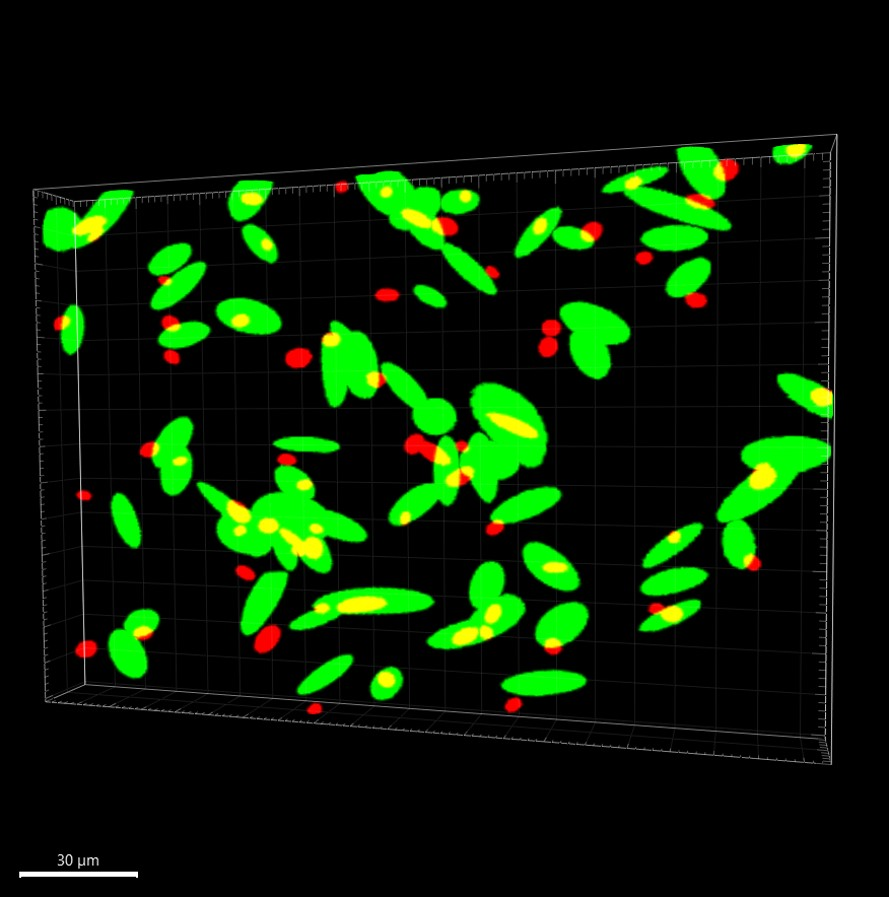
\includegraphics[width=5cm]{Images/2-mask-synthetic.jpg}}\hfil
  \subfigure[]{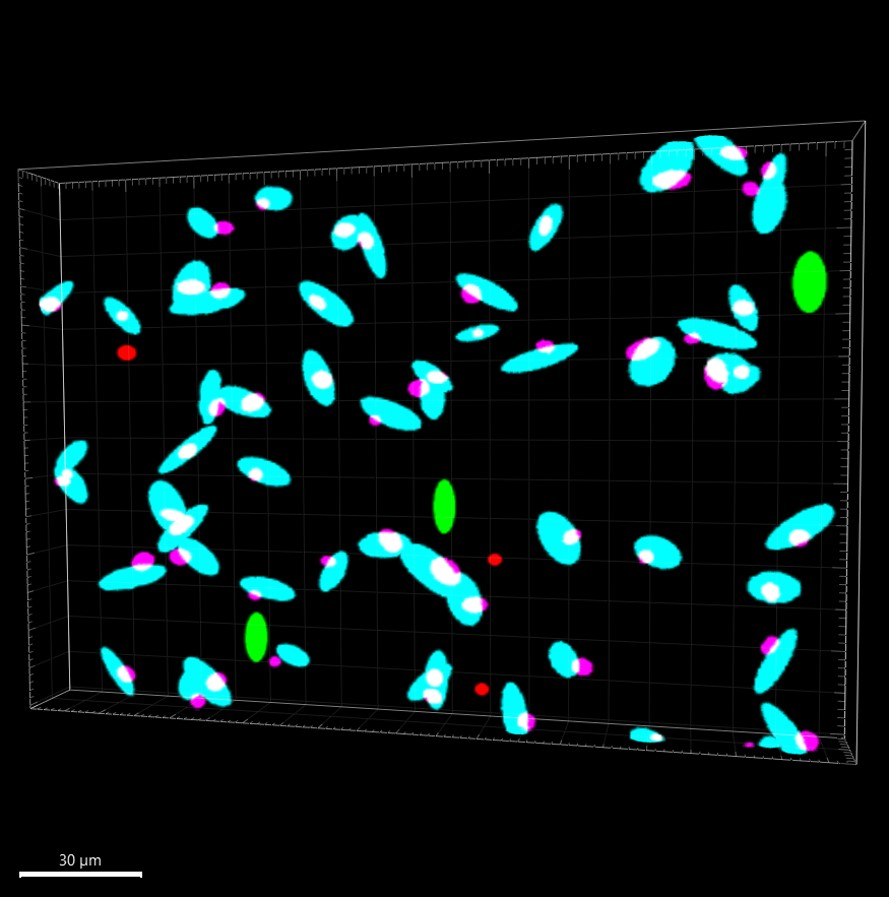
\includegraphics[width=5cm]{Images/3-mask-synthetic.jpg}}
	\caption[Example of synthetic 3D segmentation masks for: (a) 2-class segmentation task; (b) 3-class segmentation task.]{Example of synthetic \ac{3D} segmentation masks for: (a) 2-class segmentation task; (b) 3-class segmentation task.}
	\label{fig:sintetica}
\end{figure}


\section{Proposed Approach}
\label{section:proposed}

For this work, cell nuclei and Golgi semantic segmentation will be performed using the cycle-consistent GAN model, CycleGAN for short. Two different domain images will be considered, the fluorescence microscopy images (domain $I$) and the synthetic segmentation mask (domain $S$). Moreover, let $i$ and $s$ denote training examples where $i \in I$ and $s \in S$.

Like the original CycleGAN model \cite{cycleGAN:original}, the architecture of this segmentation model will be composed of four interconnected networks, two generators and two discriminators. A representation of this network can be found in Figure \ref{fig:diagrama}. The first generator ($G_S$), corresponding to the segmentation network we wish to obtain, learns a mapping from the domain $I$ to $S$. The first discriminator ($D_S$) takes the segmentation masks as input and tries to predict whether they are real or generated, according to the domain $S$. In contrast, the second generator ($G_I$) learns a mapping from the domain $S$ to $I$, and is used only to improve the training. Furthermore, the second discriminator ($D_I$) receives an image as input and predicts whether this image is real or generated, according to domain $I$.

\begin{figure}[!htb]
  \centering
  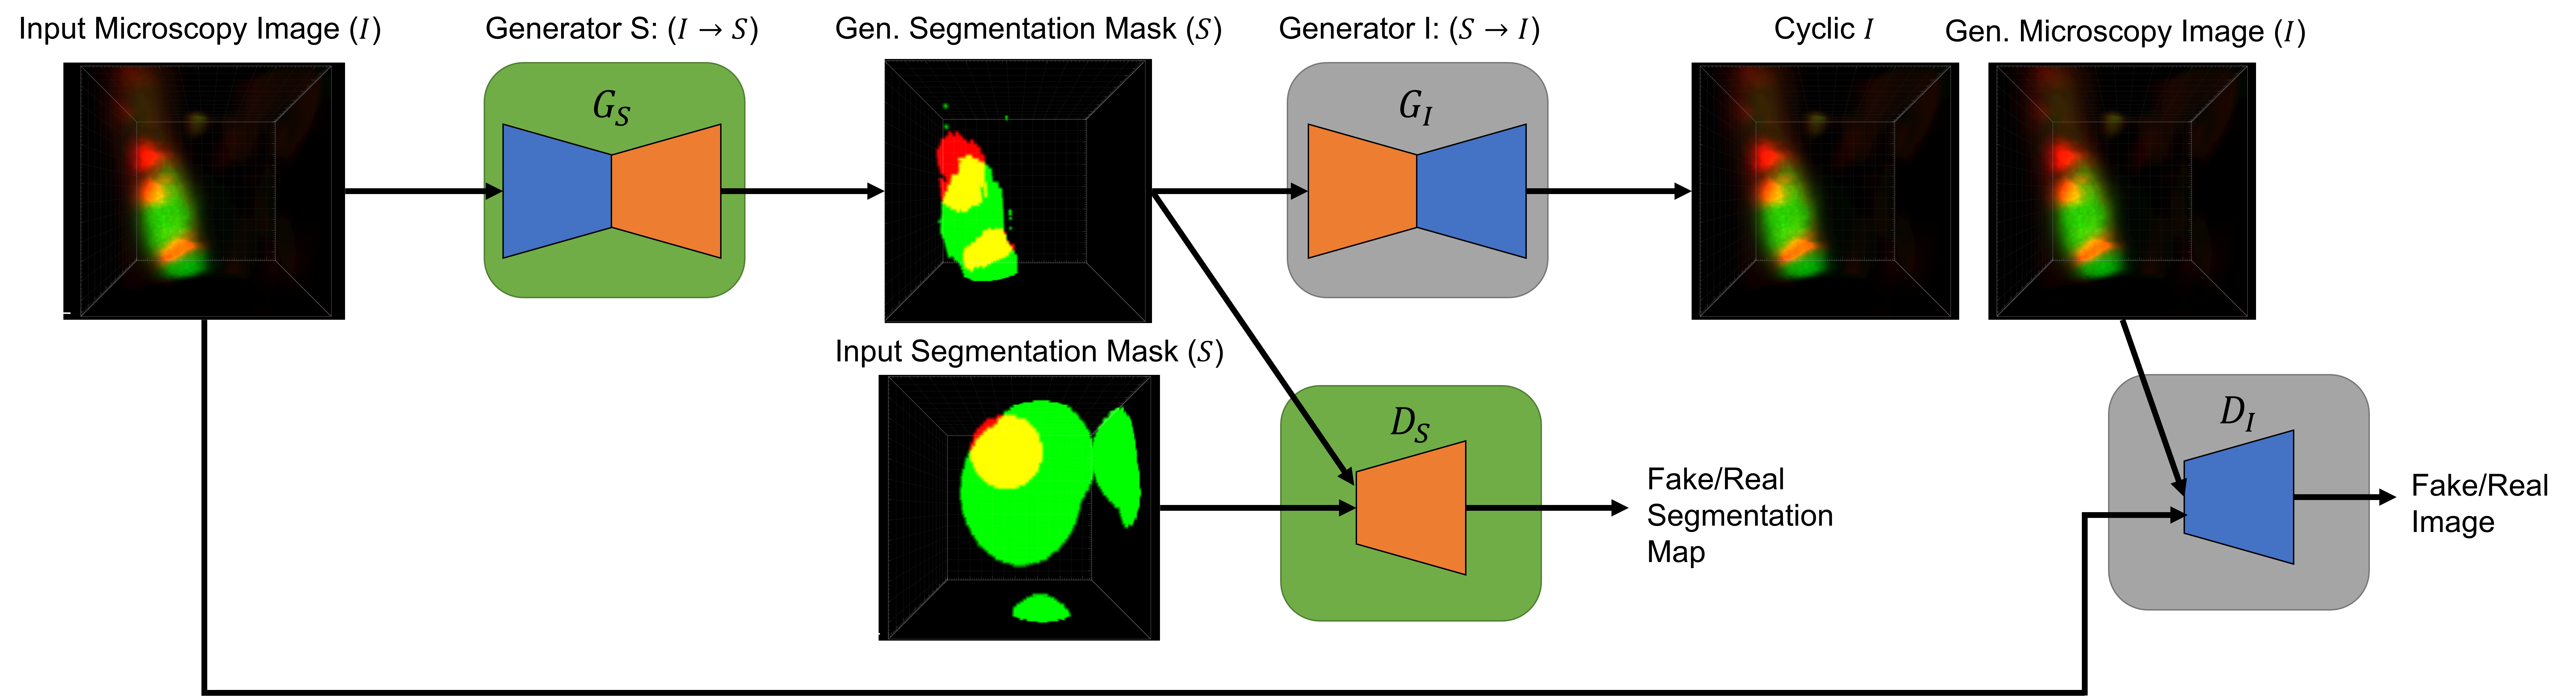
\includegraphics[width=0.99\textwidth]{Images/diagrama.jpg}
  \caption[CycleGAN schematic for the proposed approach.]{CycleGAN schematic for the proposed approach.}
  \label{fig:diagrama}
\end{figure}


\subsection*{Network Architecture}

The generator architecture used in the original CycleGAN model is intended for a \ac{2D} image-to-image translation task. Therefore, for our dataset, this approach needs to be adapted to perform a \ac{3D} image-to-image translation. This can be achieved by replacing the \ac{2D} convolutional layers of the original CycleGAN with \ac{3D} convolutional layers.  The discriminator architecture to be implemented is based on the PatchGAN \cite{isola2018imagetoimage}, which includes \ac{Leaky ReLU} for nonlinearity. The layers of the discriminator architecture must also be converted from \ac{2D} to \ac{3D}. The detailed architecture of the generator and discriminator used in the CycleGAN model employed in this work are shown in Figures \ref{fig:gencyc} and \ref{fig:disccyc}, respectively.

\begin{figure}[!htb]
  \centering
  
\includegraphics[width=0.99\textwidth]{Images/generator_cyclegan.jpg}
  \caption[Implemented CycleGAN generator architecture. The Residual Block consist of a 3D convolutional layer with instance normalization and ReLU as the activation function, followed by a second convolutional layer also with instance normalization. The output of this block is the concatenation of the output of the second layer with the input layer of the block. $k=(x,y,z)$ denotes the size of the input image for the x, y and z axes.]{Implemented CycleGAN generator architecture. The Residual Block consist of a \ac{3D} convolutional layer with instance normalization and \ac{ReLU} as the activation function, followed by a second convolutional layer also with instance normalization. The output of this block is the concatenation of the output of the second layer with the input layer of the block. $k=(x,y,z)$ denotes the size of the input image for the x, y and z axes.}
  \label{fig:gencyc}
\end{figure}

\begin{figure}[!htb]
  \centering
  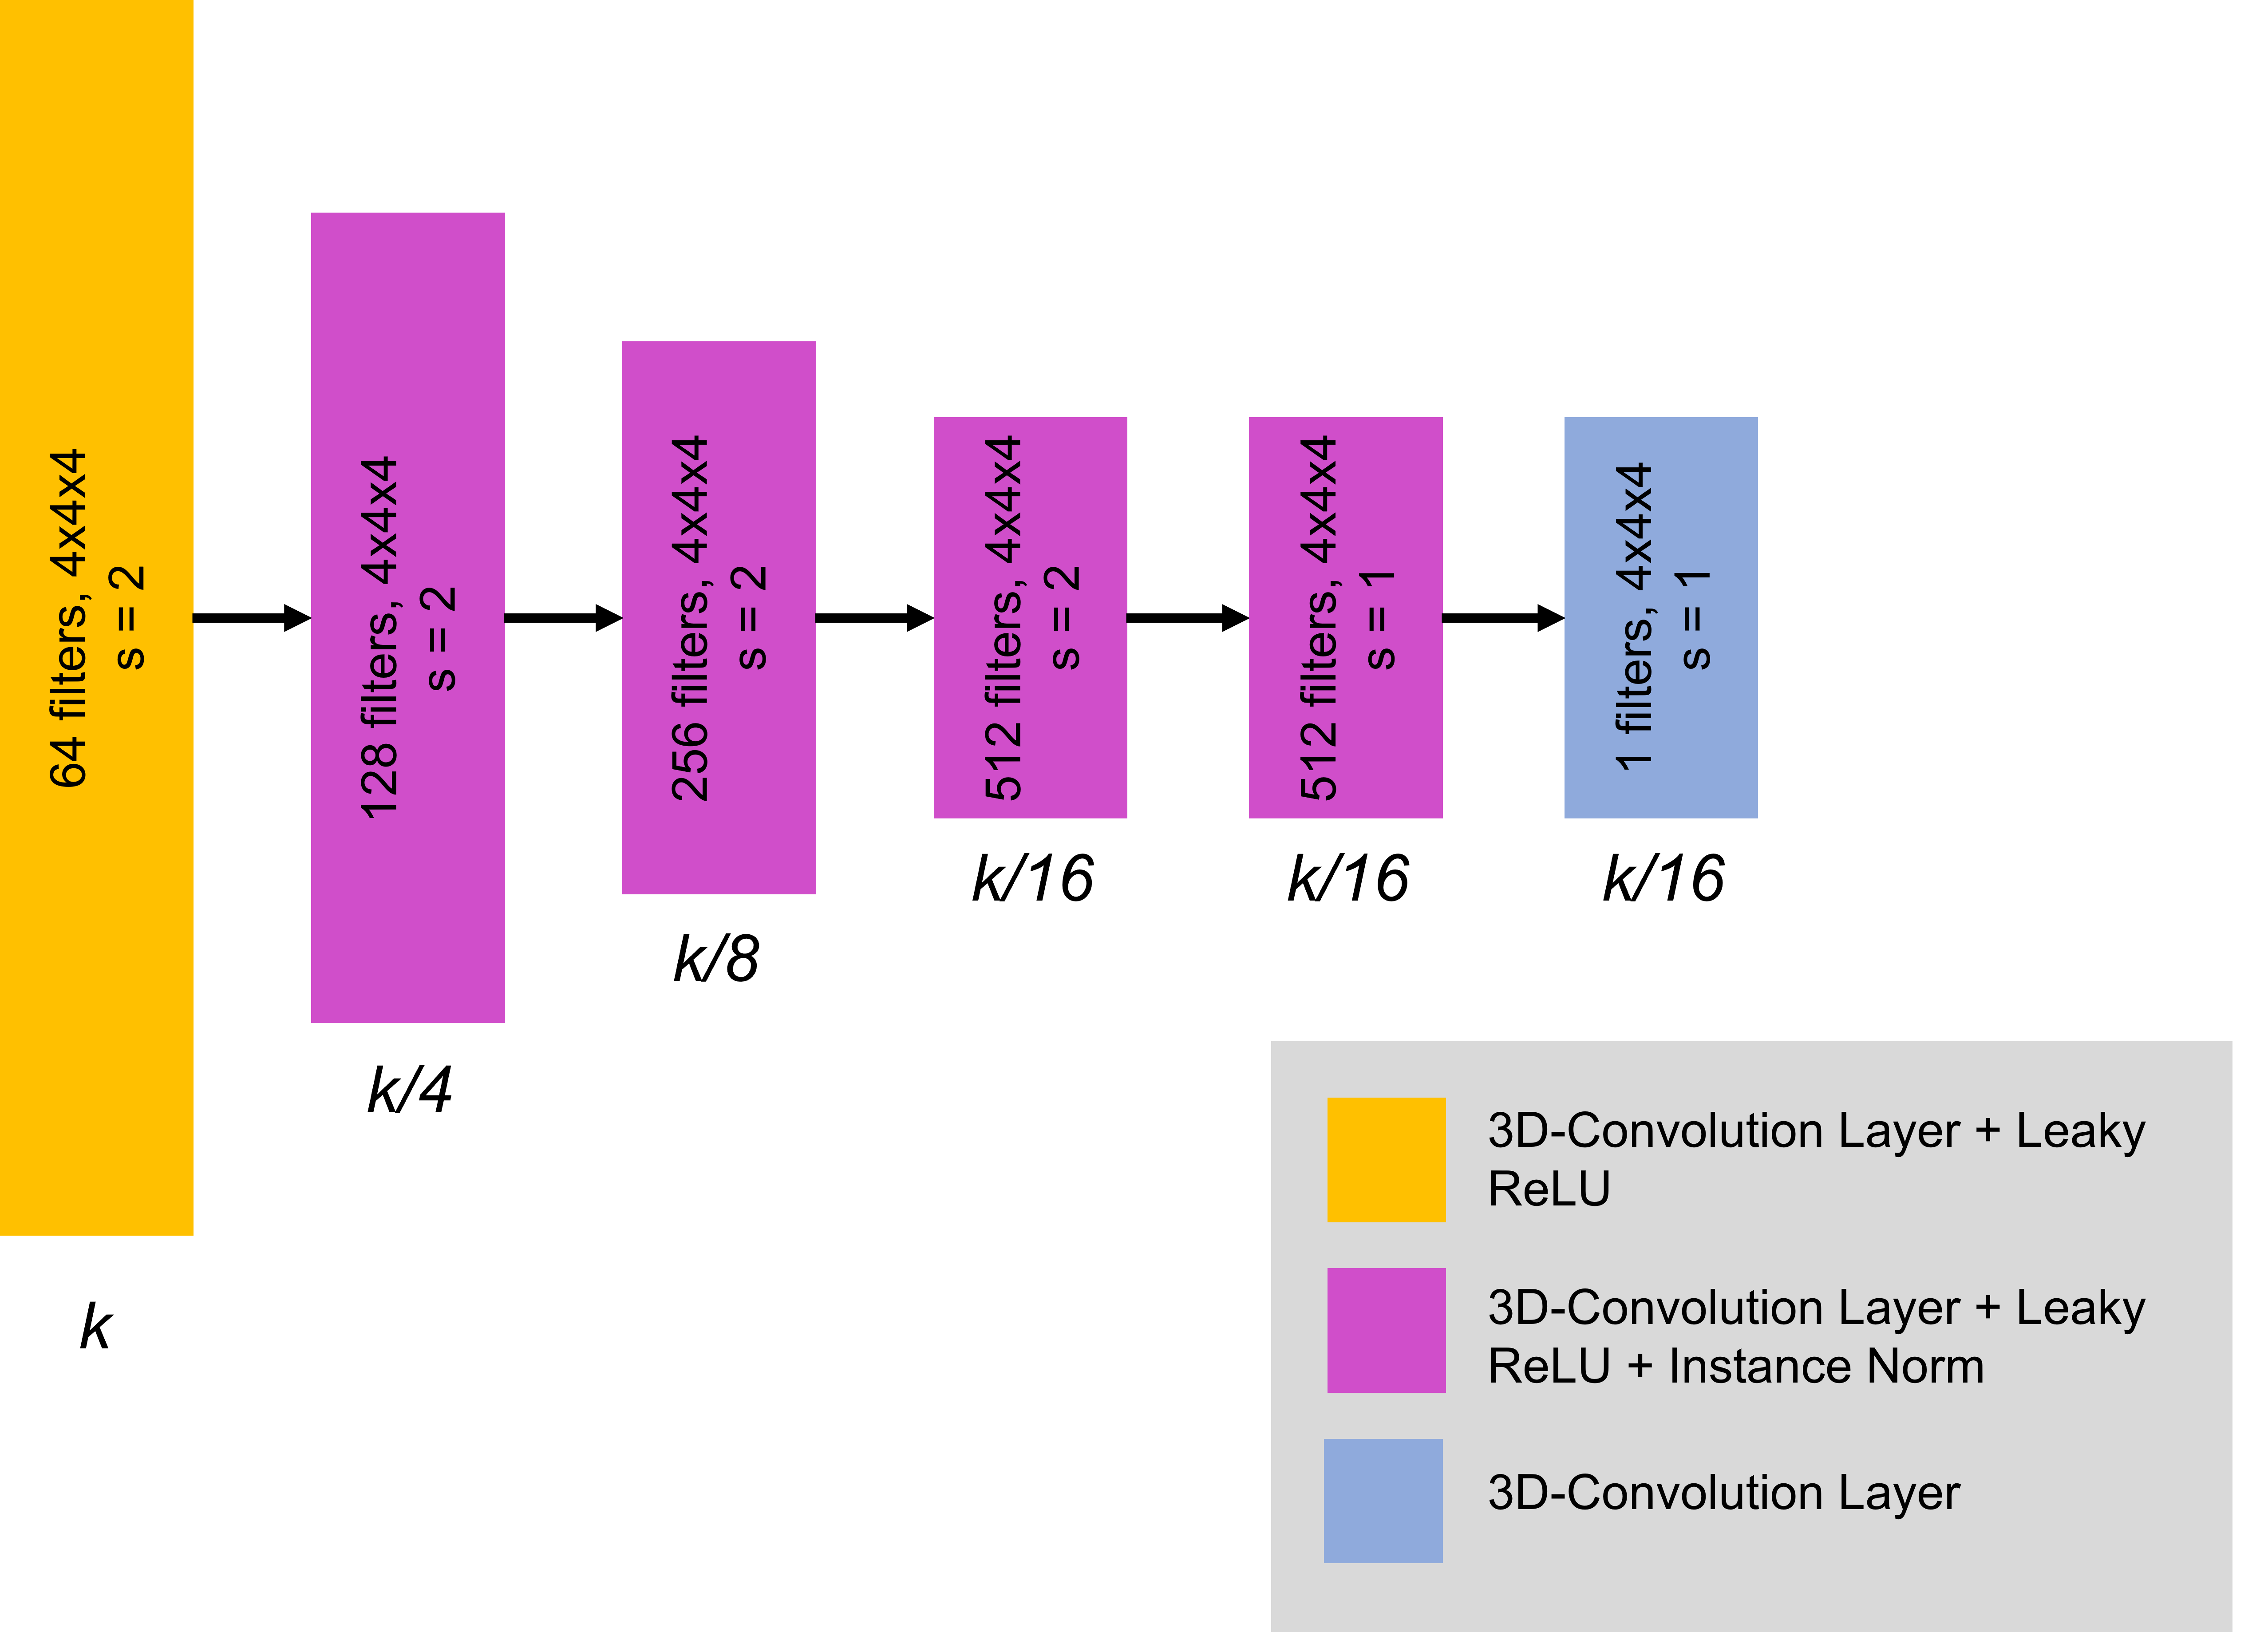
\includegraphics[width=0.50\textwidth]{Images/discriminator_cyclegan.jpg}
  \caption{Implemented CycleGAN PatchGAN discriminator architecture. $k=(x,y,z)$ denotes the size of the input image for the x, y and z axes.}
  \label{fig:disccyc}
\end{figure}

In the Figures \ref{fig:gencyc} and \ref{fig:disccyc} above, each box corresponds to a convolution block in the model. For each block, the type of convolutional layer and the normalization and activation function used after each layer are described in the Figure legend. The size of the feature map that each convolution block outputs is provided at the bottom of the boxes with respect to the size of the input image $k$. In each box, the number of filters, the size of these filters, and the stride used in each convolutional layer are indicated.

\subsection*{Loss functions}

The loss function used to train CycleGAN comprises four terms. These terms are described below.

\textbf{Adversarial Loss.} The adversarial term encourages the mapping functions to translate from one domain to
the other. First, the negative log likelihood objective from $\mathcal{L}_{GAN}$  (Equation \ref{eq:GAN}) is replaced by a least-squares loss, since according to \cite{cycleGAN:original}, this loss is more stable during training and produces higher quality results. Therefore, the adversarial loss for the first GAN ($G_{S}, D_S$), for the already mentioned notation, is given by,

\begin{equation}
    \mathcal{L}_{adv}(G_{S},D_S) = \mathbb{E}_{s \sim p_{data}(s)} [(D_S(s)-1)^2] + \mathbb{E}_{i \sim p_{data}(i)} [(D_S(G_{S}(i)))^2].
\end{equation}

The adversarial loss for the second GAN ($G_{I}, D_I$), is written as,

\begin{equation}
    \mathcal{L}_{adv}(G_{I},D_I) = \mathbb{E}_{i \sim p_{data}(i)} [(D_I(i)-1)^2] + \mathbb{E}_{s \sim p_{data}(s)} [(D_I(G_{I}(s)))^2].
\end{equation}

\textbf{Cycle consistency loss.} The cycle consistency loss, $\mathcal{L}_{cyc}$, was described in subsection \ref{subsection:CycleGAN} with an expression given by (\ref{eq:CCL}). Transferred to our notation, it has the following form,

\begin{equation} 
\mathcal{L}_{cyc} = \mathbb{E}_{i \sim p_{data}(i)} [||G_{I}(G_{S}(i))-i||_1] + \mathbb{E}_{s \sim p_{data}(s)} [||G_{S}(G_{I}(s))-s||_1].
\label{eq:cly_2}
\end{equation}

\textbf{Identity mapping loss.} Lastly, the identity mapping loss, $\mathcal{L}_{id}$ has also been described in subsection \ref{subsection:CycleGAN} with an expression given by (\ref{eq:identity}). Transferred to our notation, it has the following form,

\begin{equation}
    \mathcal{L}_{id} = \mathbb{E}_{i \sim p_{data}(i)} [||G_{I}(i)-i||_1] +  \mathbb{E}_{s \sim p_{data}(s)} [||G_{S}(s)-s||_1].
\end{equation}

Finally, the total loss is obtained by combining by combining the 4 terms:

\begin{equation}
\label{eq:total-cyclegan-loss}
    \mathcal{L}(G_{S},G_{I},D_S,D_I) = \mathcal{L}_{adv}(G_{S},D_S) + \mathcal{L}_{adv}(G_{I},D_I) + \lambda_{cyc} \mathcal{L}_{cyc} + \lambda_{id} \mathcal{L}_{id}
\end{equation}

\noindent where $\lambda_{cyc}$ and $\lambda_{id}$ are hyperparameters to optimize that control the relative importance of the two objectives. Thus, the objective function is:

\begin{equation}
    \arg \min_{G_{S},G_{I}}\max_{D_S,D_I} \mathcal{L}(G_{S},G_{I},D_S,D_I).
\end{equation}

\section{Comparison between different approaches}
\label{section:comparison}

The performance of the proposed approach will be compared with two other known supervised techniques for segmenting nuclei and Golgi in fluorescence microscopy images, the \ac{3D} U-Net \cite{Unet:3D} and Vox2Vox, which is the \ac{3D} extension of the Pix2Pix model \cite{isola2018imagetoimage}. To train these models, the \ac{3D} volumes of fluorescence microscopy images and corresponding \ac{3D} segmentation masks are required.

The following subsections provide information on the implementation of these methods.

\subsection{3D U-Net}

The \ac{3D} U-Net architecture is used to predict two binary segmentation maps, one for the nuclei and other for the Golgi.

The implemented architecture, based on the one described in Section \ref{section:CNN&UNET} (Figure \ref{fig:3dUnet}), is demonstrated in Figure \ref{fig:y-unet-3d}.

\begin{figure}[!htb]
  \centering
  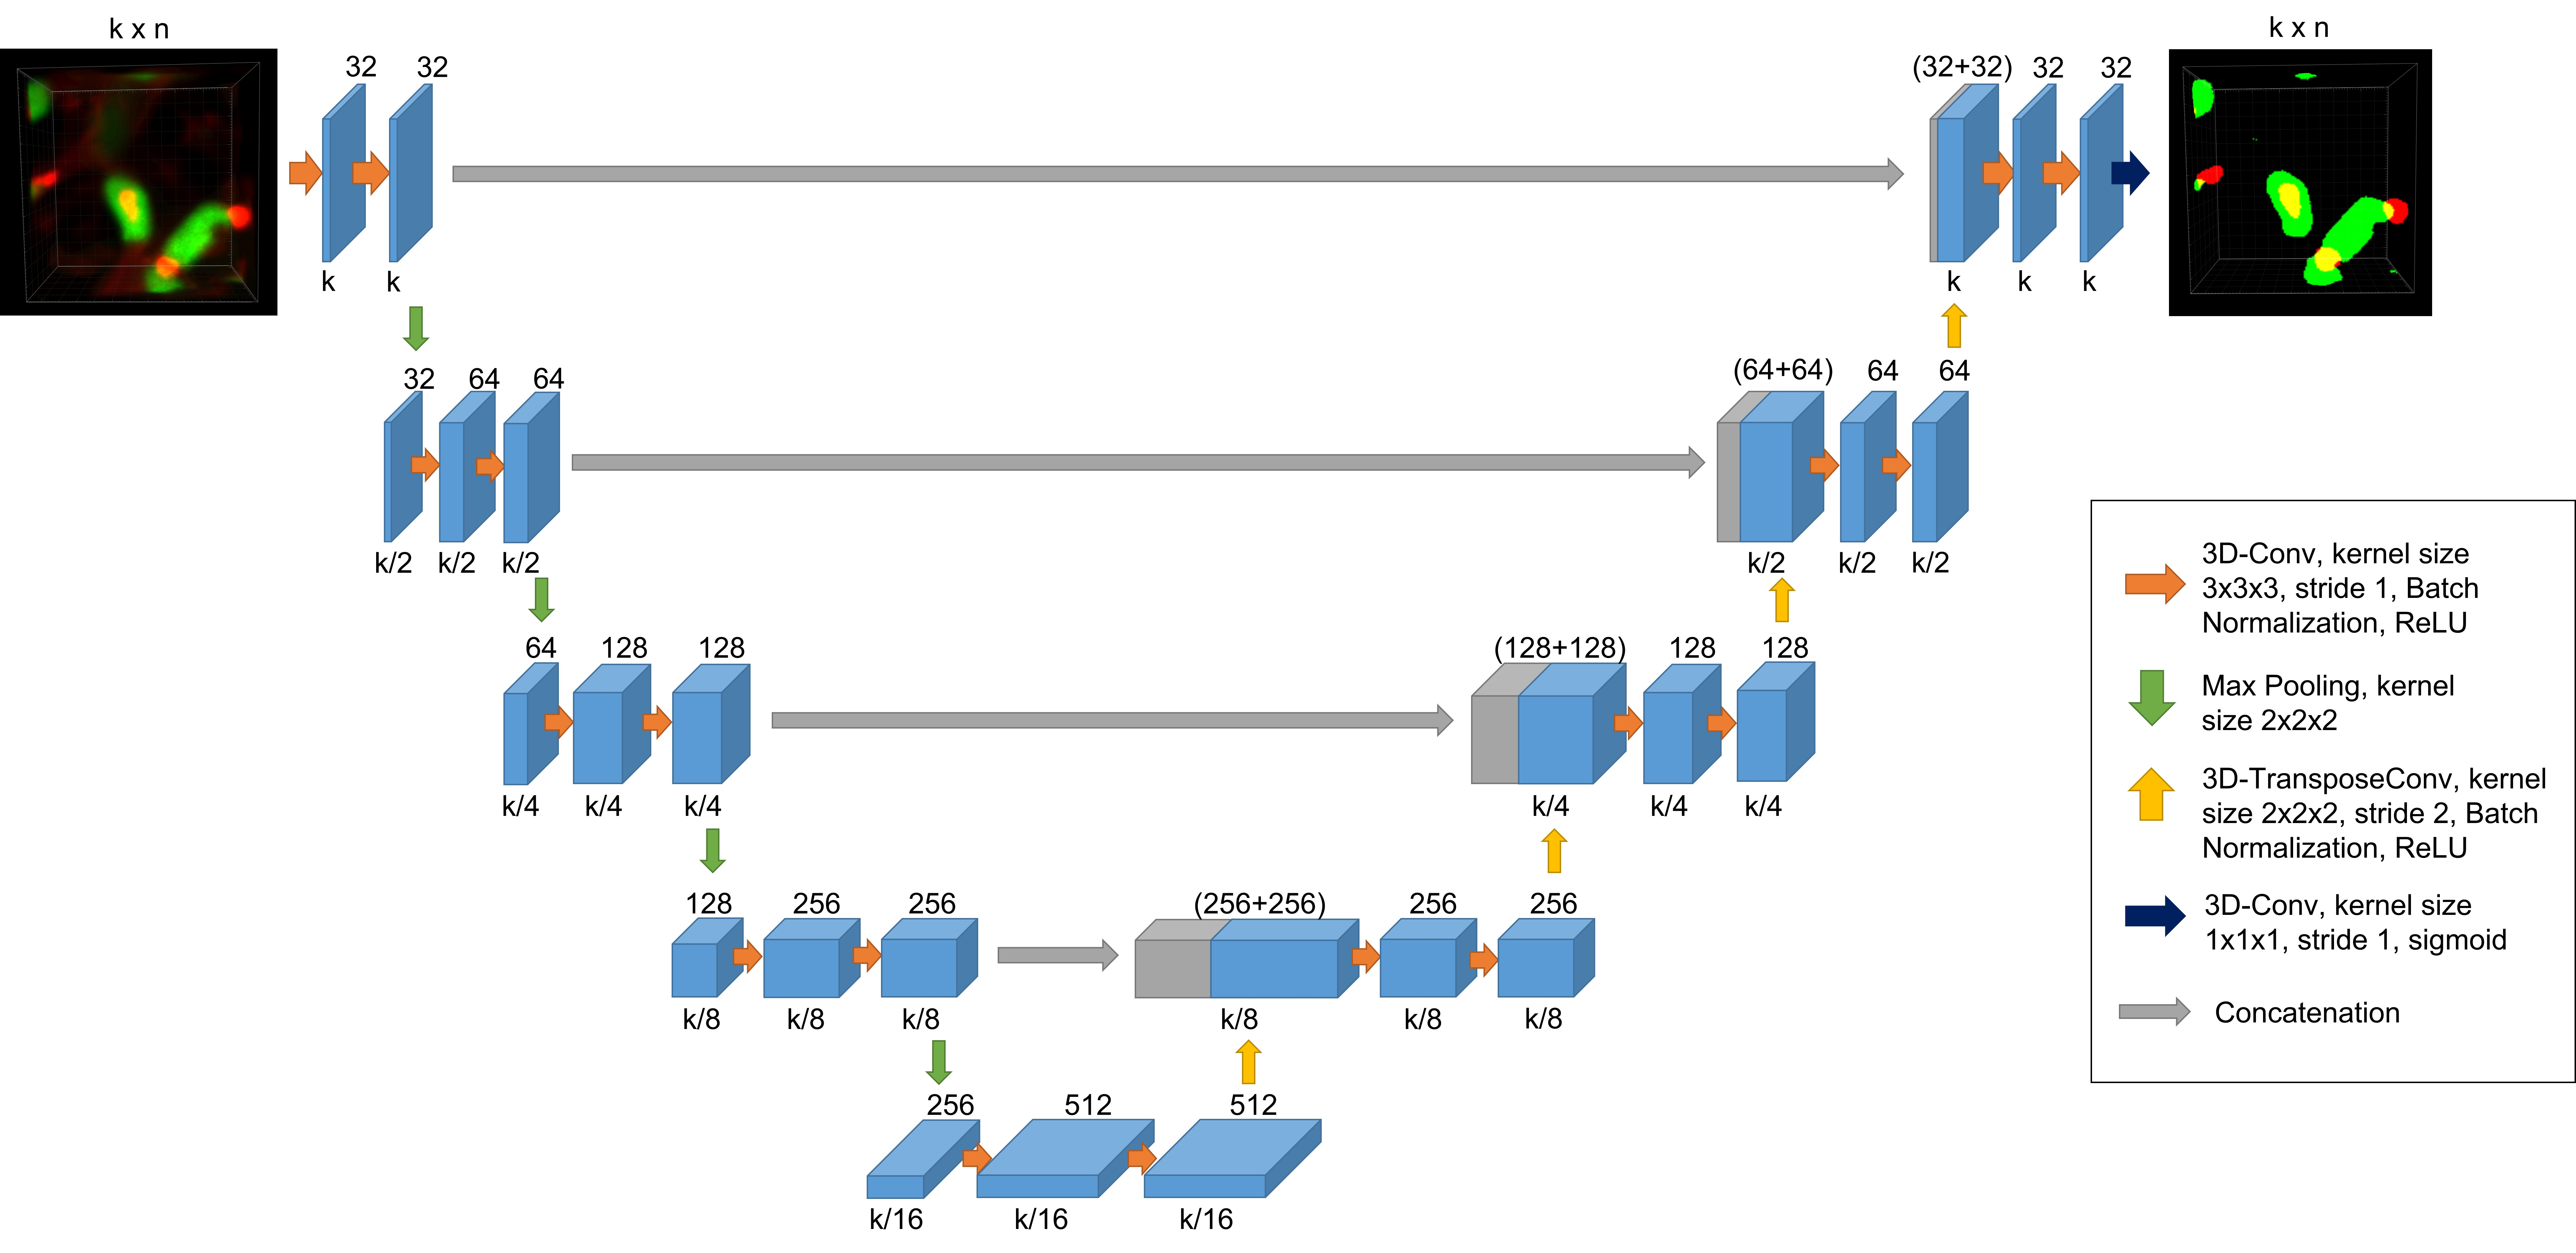
\includegraphics[width=0.85\textwidth]{Images/Picture1.jpg}
  \caption{Implemented \ac{3D} U-Net architecture. $k=(x,y,z)$ denotes the size of the input image for the x, y and z axes. $n$ denores the number of input/output channels.}
  \label{fig:y-unet-3d}
\end{figure}

In the Figure above, each blue box corresponds to a multi-channel feature map. The number of channels is indicated at the top of the box. The size of the feature map is provided at the bottom of the box with respect to the size of the input image $k$. Grey boxes represent copied feature maps. The arrows denote the different operations. The $n$ (above the input and output images) is the number of channels of the input and output images, $n$=2 and $n$=3 for the 2-class and 3-class segmentation tasks, respectively. The output image in the Figure is an example of the output for the 2-class segmentation task.

The \ac{DC} is a widely used metric in the computer vision community to calculate the similarity between two images \cite{diceloss}. Therefore, the dice coefficient has been fitted to a loss function known as \ac{DLoss}:

\begin{equation}
    DLoss(y,\hat{p}) = 1 - \frac{2y\hat{p}+1}{y+\hat{p}+1}
    \label{eq:dice-loss}
\end{equation}

\noindent here $y$ is the reference value, $\hat{p}$ is the probability value predicted by the model and 1 is added to both the numerator and denominator to ensure that the function is not undefined in edge case scenarios, e.g., when $y=\hat{p}=0$. Unlike the original \ac{3D} U-Net model \cite{Unet:3D} previously described in Section \ref{section:CNN&UNET}, the loss function used in training the model is the Dice loss represented in equation \ref{eq:dice-loss}.

\subsection{Vox2Vox}

Pix2Pix is a supervised GAN model designed for image-to-image translation, previously described in subsection \ref{subsection:pix2pix}. However, it is not capable of performing image-to-image translation at the \ac{3D} level. A \ac{3D} volume-to-volume network for segmentation used as an alternative to Pix2Pix is the Vox2Vox network.

\citet{vox2vox} used a Vox2Vox approach in their work. For this work, it will be used a similar architecture. The generator model is built in the style of the U-Net and Res-Net \cite{2015deep} architectures, while the discriminator is built in the style of the PatchGAN \cite{isola2018imagetoimage}  architecture. The implemented architectures are shown in Figures \ref{fig:genvox} and \ref{fig:discvox}.

\begin{figure}[!htb]
  \centering
  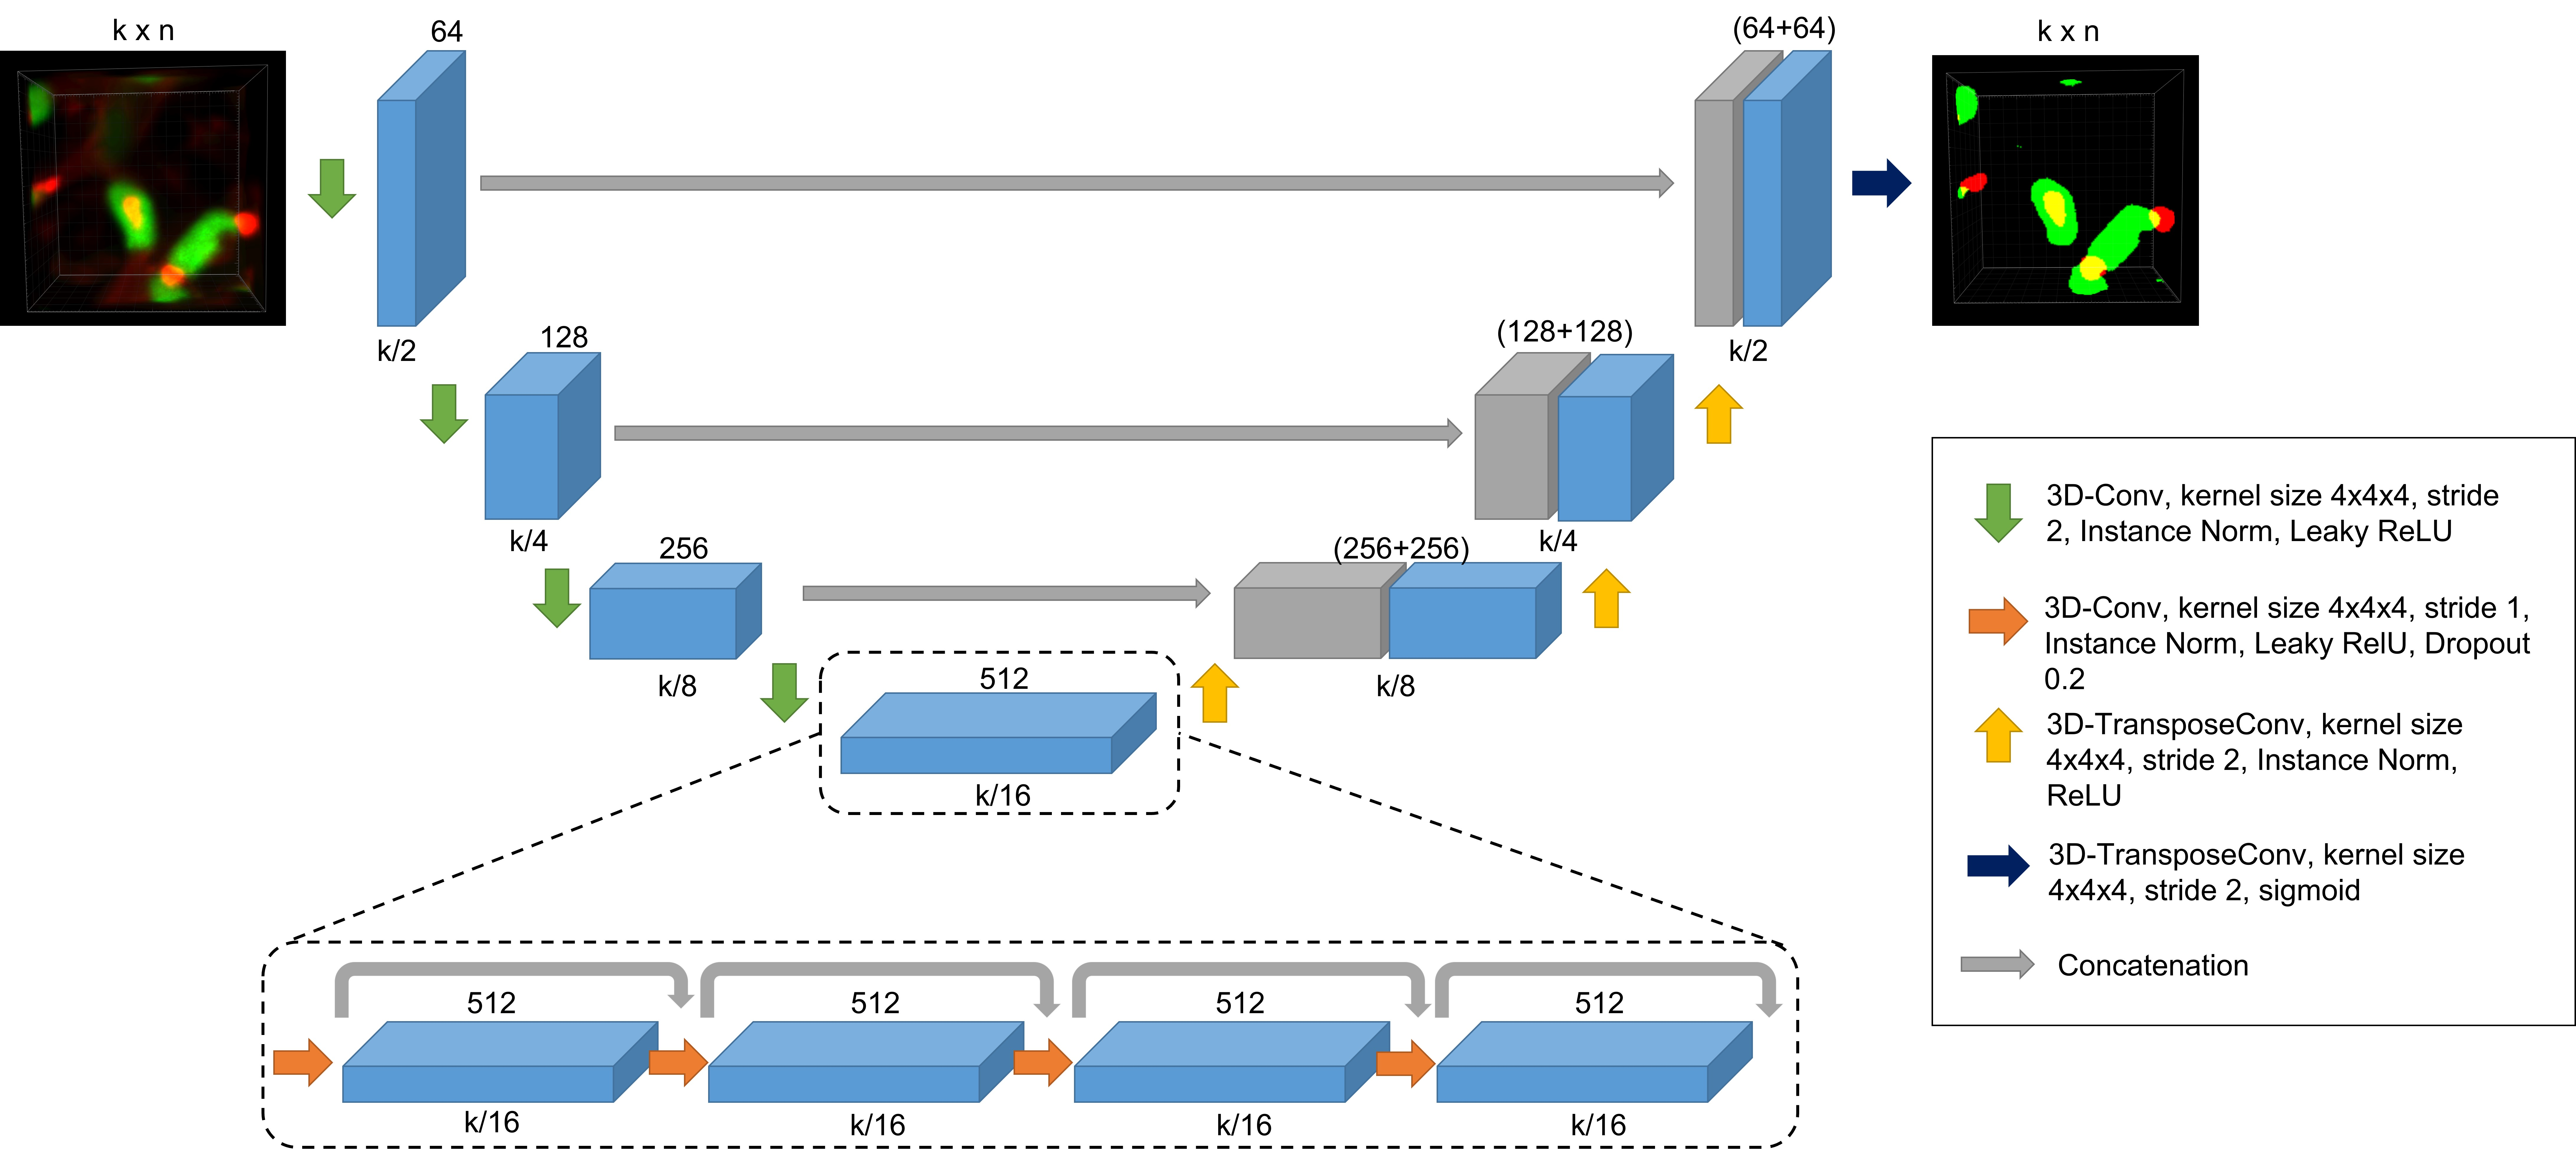
\includegraphics[width=0.85\textwidth]{Images/Picture2.jpg}
  \caption[Implemented Vox2Vox generator architecture.]{Implemented Vox2Vox generator architecture. $k=(x,y,z)$ denotes the size of the input image for the x, y and z axes. $n$ denores the number of input/output channels.}
  \label{fig:genvox}
\end{figure}

\begin{figure}[!htb]
  \centering
  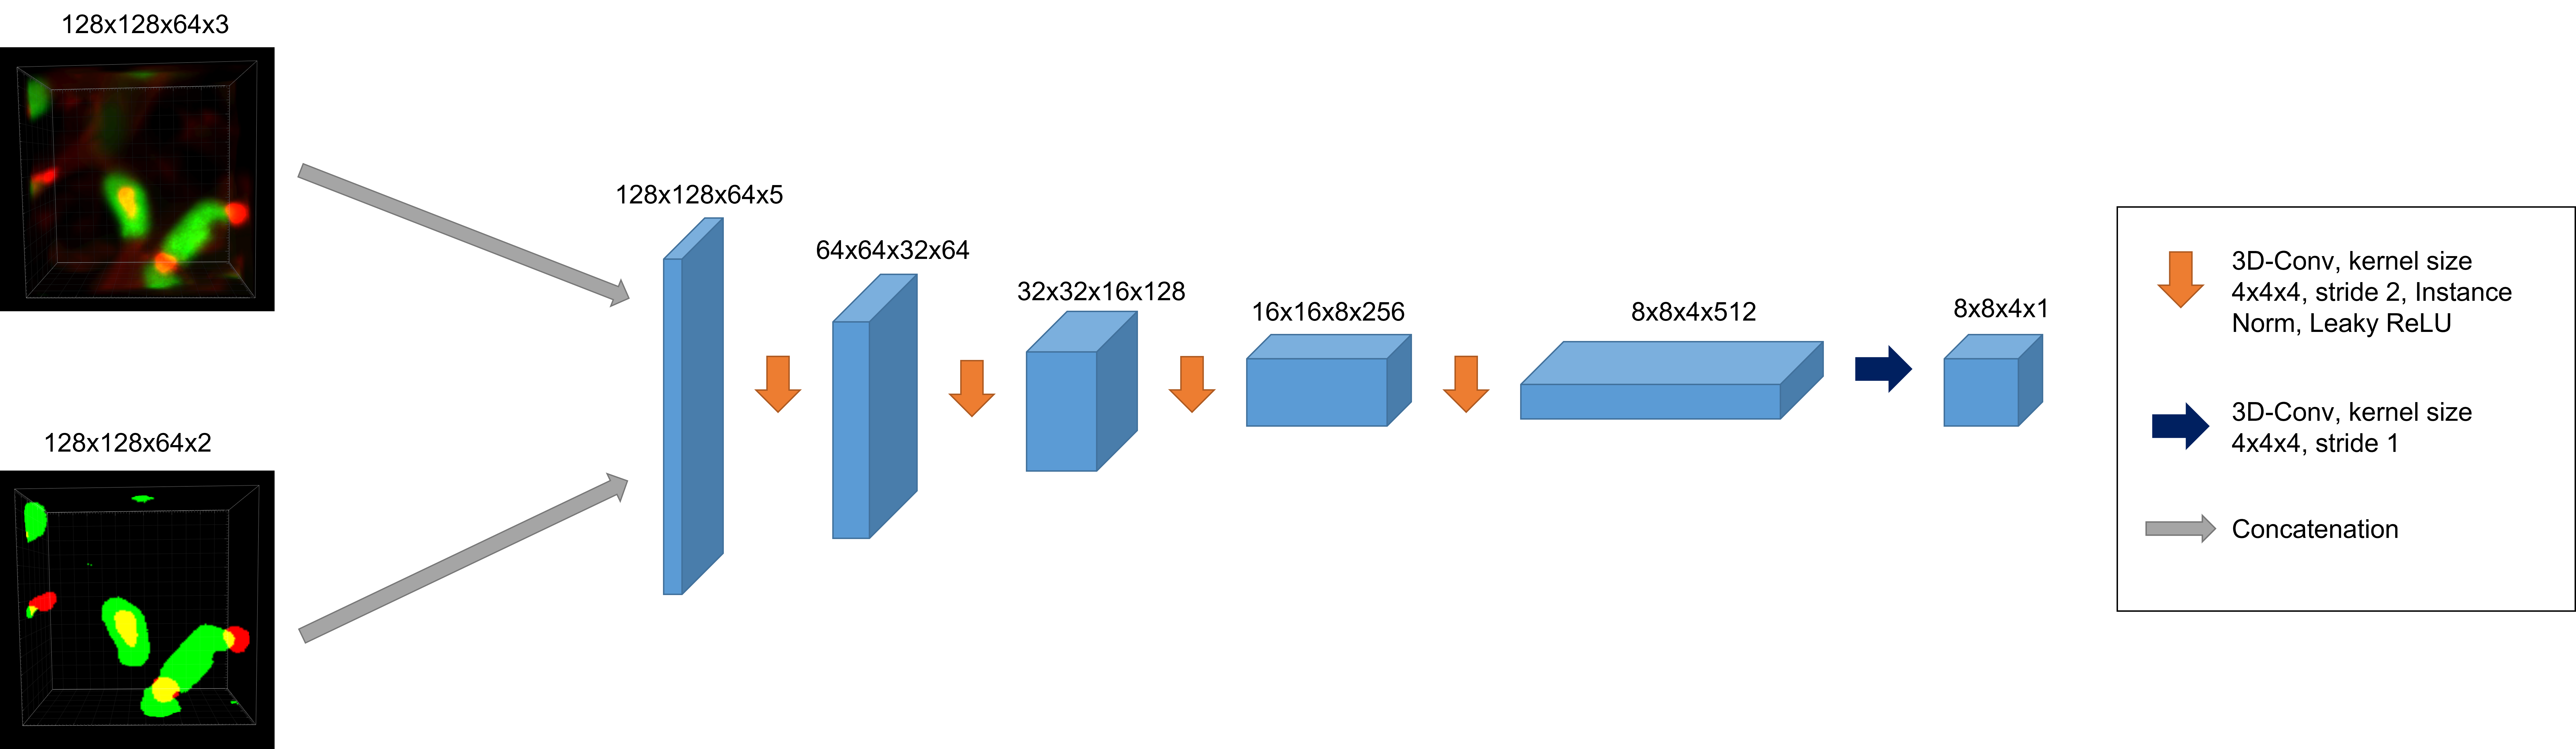
\includegraphics[width=0.90\textwidth]{Images/discriminator_vox.jpg}
  \caption[Implemented Vox2Vox discriminator architecture.]{Implemented Vox2Vox discriminator architecture. $k=(x,y,z)$ denotes the size of the input image for the x, y and z axes. $n$ denores the number of input/output channels.}
  \label{fig:discvox}
\end{figure}

In the Figures \ref{fig:genvox} and \ref{fig:discvox}, each blue box corresponds to a multi-channel feature map. The number of channels is indicated at the top of the box. The size of the feature map is provided at the bottom of the box with respect to the size of the input image $k$. Grey boxes represent copied feature maps. The arrows denote the different operations. The $n$ (above the input and output images in the generator architecture) is the number of channels of the input and output images. The output of the generator architecture is an example of the output for the 2-class segmentation task.

Another important part of the implementation of Vox2Vox model is the loss function. The discriminator loss, $\mathcal{L}_{disc}$, is the sum of the $L_2$ error of the discriminator output between the original image $x$ and the respective ground-truth $y$ with a tensor of ones, and the $L_2$ error of the discriminator output between the original image and the respective segmentation prediction $\hat{y}$ given by the generator with a tensor of zeros. This can be formulated as follows:

\begin{equation}
    \mathcal{L}_{disc} = L_2[D(x,y),\boldsymbol{1}] + L_2[D(x,\hat{y}),\boldsymbol{0}].
\end{equation}

On the other hand, the generator loss, $\mathcal{L}_{gen}$, is the sum of the $L_2$ error of the discriminator output between the original image, $x$, and the corresponding segmentation prediction, $\hat{y}$, with a tensor of ones, and the \ac{DLoss}, between the ground-truth and the generator output multiplied by the scalar weight coefficient $\alpha > 0$. This can be formulated in the following way:

\begin{equation}
\label{eq:vox2vox-generator-loss}
    \mathcal{L}_{gen} = L_2[D(x,\hat{y}),\boldsymbol{1}] + \alpha DLoss(y,\hat{y}).
\end{equation}

\section{Models Inference}
\label{section:models_inference}

As indicated in Section \ref{section:dataset}, the input size of the proposed models is 64x64x64. Therefore, to obtain the predicted segmentation mask of an entire crop, it is necessary to slide a \ac{3D} window of size 64x64x64 to segment the entire crop. To make the segmentation mask the same size as the original crop, we need to pad the X and Y axes of the original image so that the dimensions are $X_{pad} = (X \% step) \times step $ and $Y_{pad} = (Y \% step) \times step $, where $step$ is the number of pixels the \ac{3D} window moves during inference. The padding used is reflection padding. If you place a \ac{3D} window in the upper left corner of the padded crop a 64x64x64 patch becomes the input volume of the model used to create a sub-volume of the segmentation mask in the upper left. This \ac{3D} window is slid in x and y direction with a certain $step$ through the entire padded crop until the entire volume is processed.



\section{Execution time}
\label{section:execution_time}

The execution time of a deep neural network model can be divided into two intervals: the training time and the testing time. Here, the training time corresponds to the time it takes for a model to learn a particular task. The test time is the time required for a model to make a segmentation prediction for an image. In this work, the execution time is also considered as a measure of the performance of the different approaches. For supervised methods that require manual annotations, the time required to create these masks is also considered.
% If Printing on DOUBLE SIDED pages, the second page should be white.
% Otherwise, comment the following command:
\cleardoublepage
%
%Chapter 5
% #############################################################################
% This is Chapter 5
% !TEX root = ../main.tex
% #############################################################################
% Change the Name of the Chapter i the following line
\fancychapter{Experimental Results and Discussion}
\cleardoublepage
% The following line allows to ref this chapter
\label{chap:results}

% Introductory text

This chapter presents the experimental results and discussion regarding the segmentation of cell nuclei and Golgi in fluorescence microscopy images.


\section{Computational Environment}

In this work, all deep learning implementations are based on the open-source deep learning libraries Tensorflow and Keras \cite{tensorflow,keras}. Tensorflow is an end-to-end machine learning platform that makes it easy to build and train machine learning models. Keras is a high-level application programming interface (API) of Tensorflow. In addition, all experiments were performed in Python 3.9 on a computer with the following specifications:

\begin{itemize}
    \itemsep0em 
    \item Processor: Intel(R) Core(TM) i5-8400 CPU @ 2.80GHz;
    \item Memory: 16 GB RAM;
    \item Storage: 250 GB SSD + 1 TB HDD;
    \item Graphics Processing Unit (GPU): NVIDIA GeForce GTX 1070 with 8 GB of VRAM.
\end{itemize}


\section{Data Pre-Processing}
\label{section:pre}
This section presents the pre-processing methods applied to the images in the dataset presented in section \ref{section:dataset}.

From the histogram of intensity values in figure \ref{fig:micro} of one of the microscopic images from the dataset, it's possible to verify that most of the pixels in the red and green channels have low intensity values. To correct this, we need to manipulate the intensity histogram of the image, which can be done by contrast stretching.

\begin{figure}[!htb]
  \centering
  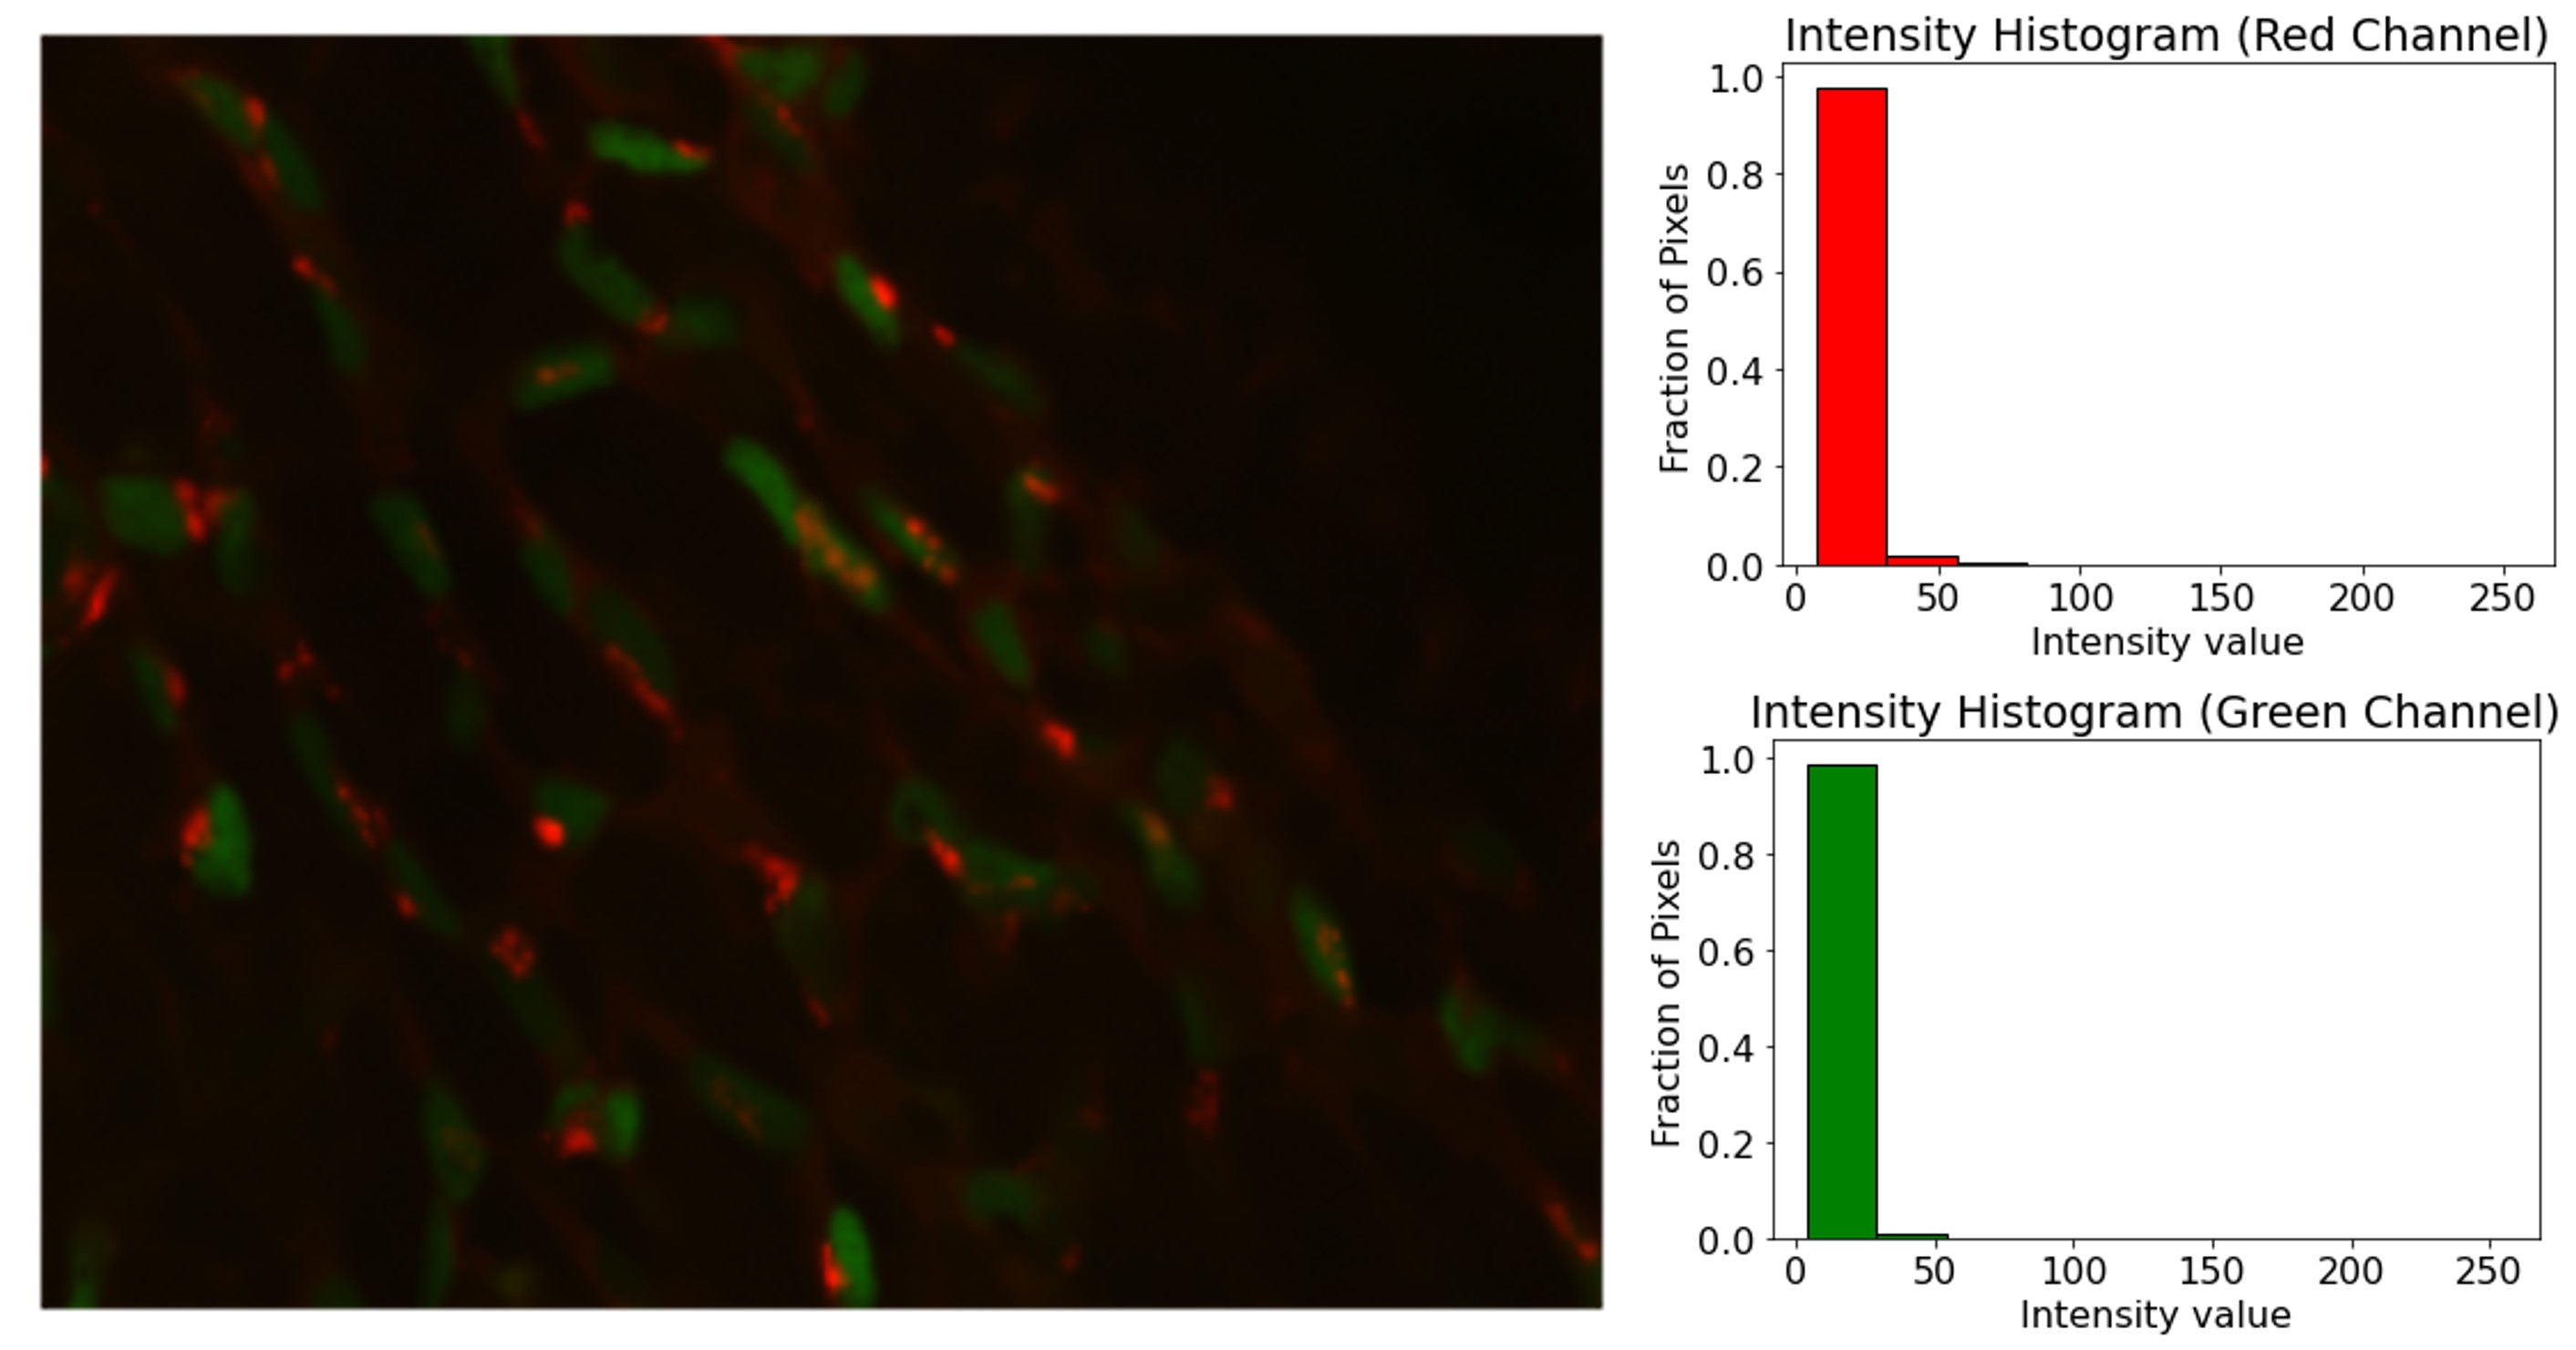
\includegraphics[width=0.75\textwidth]{Images/img.jpg}
  \caption[Slice of microscopic image from the dataset.]{Slice of microscopic image from the dataset.}
  \label{fig:micro}
\end{figure}

% https://www.notilyze.com/en/news/improving-object-detection-with-contrast-stretching-part-1-2/

Contrast stretching should theoretically improve the learning ability of models by highlighting the contours of objects and emphasizing the difference between object and background. This helps convolutional layers extract information and features from images \cite{contrast_strect}. Contrast stretching can be easily done for an image using a formula that scales up the differences in pixel values. This up scaling must be applied to all color channels, so for the microscopic images used in this work, it must be applied to the red and green channels (as mentioned earlier, these images have no blue channel).

The contrast stretching can be done by transforming pixel $x$ following formula:

\begin{equation}
    \label{eq:contrast}
    f(x) = \frac{x-a}{b-a} \times 255
\end{equation}


\noindent where $a$ is the lower limit to scale to, and $b$ is the upper limit. Instead of using the minimum and maximum values in the contrast stretch as the lower and upper bounds, the 5 and 98 percentile values are used, respectively. These values were chosen by visual inspection of the pre-processing results considering different percentile values. The values that best enhance the contrast of the Golgi and nuclei were selected.

The results of this process can be found in figure \ref{fig:micro_pre} and, together with the corresponding new intensity histograms for the red and green channels.

\begin{figure}[!htb]
  \centering
  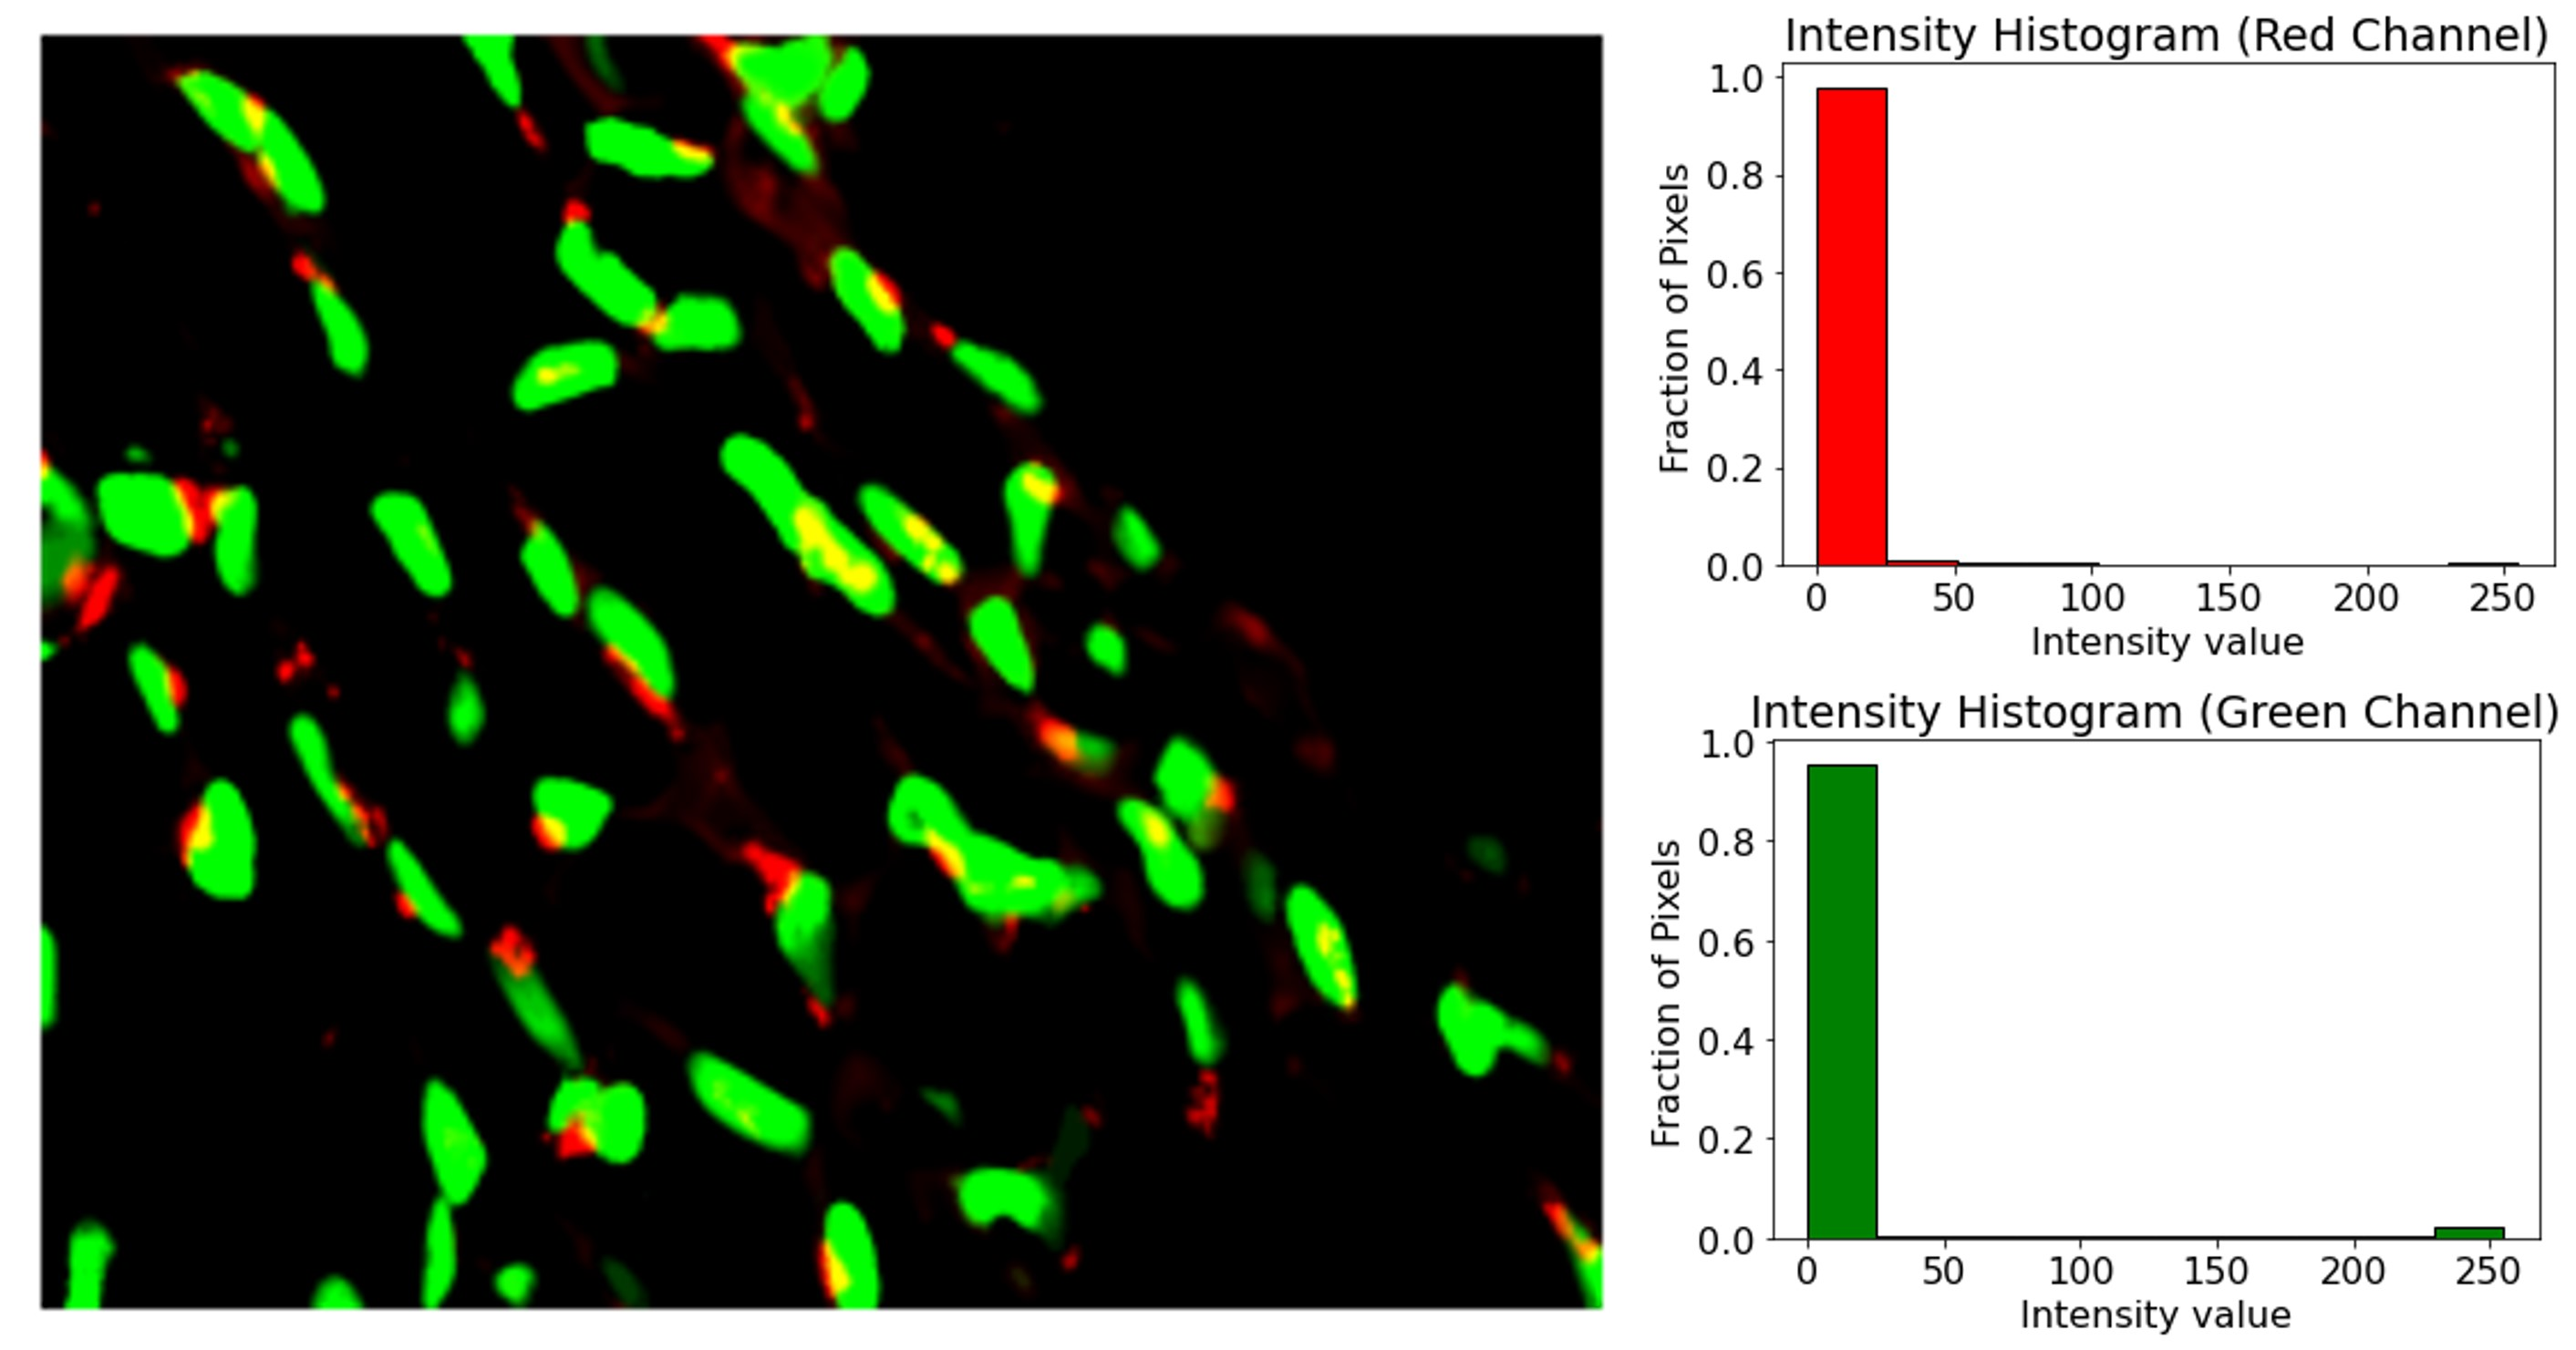
\includegraphics[width=0.75\textwidth]{Images/pre.jpg}
  \caption[Same image slice of figure \ref{fig:micro} after percentile contrast stretching.]{Same image slice of figure \ref{fig:micro} after percentile contrast stretching.}
  \label{fig:micro_pre}
\end{figure}


Another simple step of the data pre-processing method applied to the dataset of microscopic images was to normalize the input images with values in the range [0,255] to values in the interval [0,1] by dividing each image value by 255. This process is important because when the original images are used as input of the Deep Neural Networks, computing these high numerical values requires a lot of computational resources and time. When the data is normalized, the pixel values are smaller, so the computational resources and time required to converge the model are greatly reduced.

\section{Implementation Details, Results and Discussion}

In this section the experimental results regarding the segmentation of cell nuclei and Golgi in fluorescence microscopy images obtained with the proposed models are presented and discussed. In each subsection, a different model is described and each subsection is divided into two parts. In \textbf{2 Class}, the results obtained for the models predicting two output probability maps (for nuclei and Golgi) are presented, and in \textbf{3 Class}, the results obtained for the models predicting three output probability maps (nuclei, Golgi and nucleus-Golgi pairs) are presented.

All models are tested on two of the eight crops in the dataset described in section \ref{section:dataset}. Shown in figure \ref{fig:dataset} are: the original test crops in (a) and (e), designated $I^{orig}_1$ and $I^{orig}_2$, respectively; the crops obtained by applying the pre-processing method described in the previous section in (b) and (f), designated $I^{Pre}_1$ and $I^{Pre}_2$, respectively; the ground truth segmentation masks for the models with 2 output channels in (c) and (g), denoted $I^{gt}_{21}$ and $I^{gt}_{22}$, respectively; and the ground truth segmentation masks for the models with 3 output channels in (d) and (h), denoted $I^{gt}_{31}$ and $I^{gt}_{32}$, respectively.

\begin{figure}[!htb]
\centering
\subfigure[]{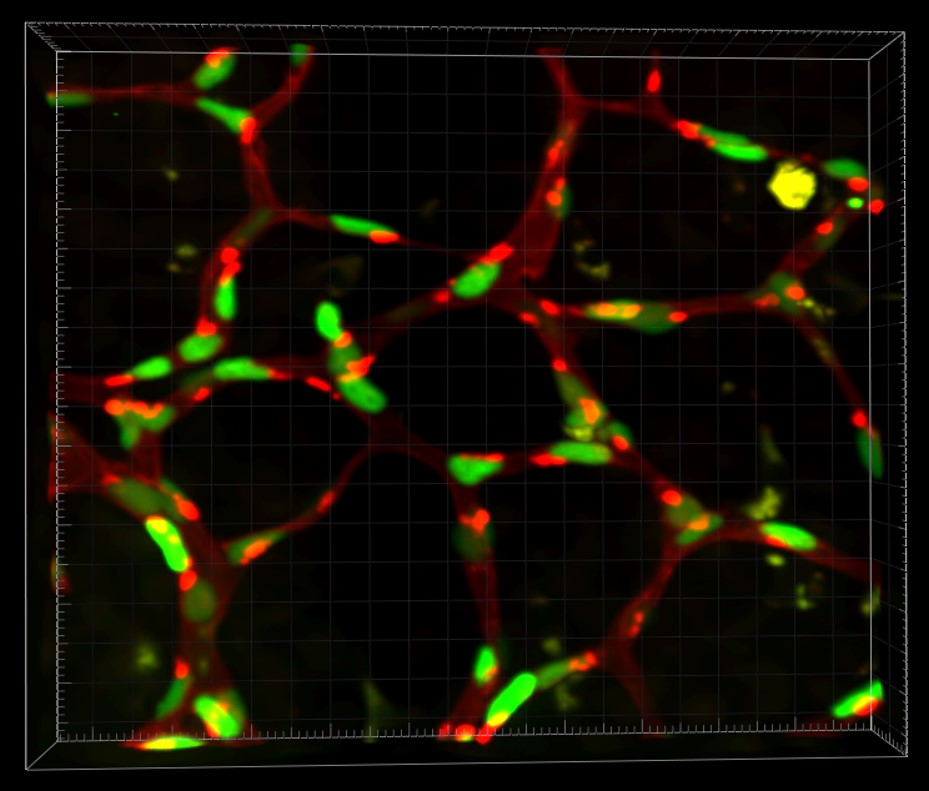
\includegraphics[width=3.5cm]{Images/crop5_img.jpg}}\hfil
\subfigure[]{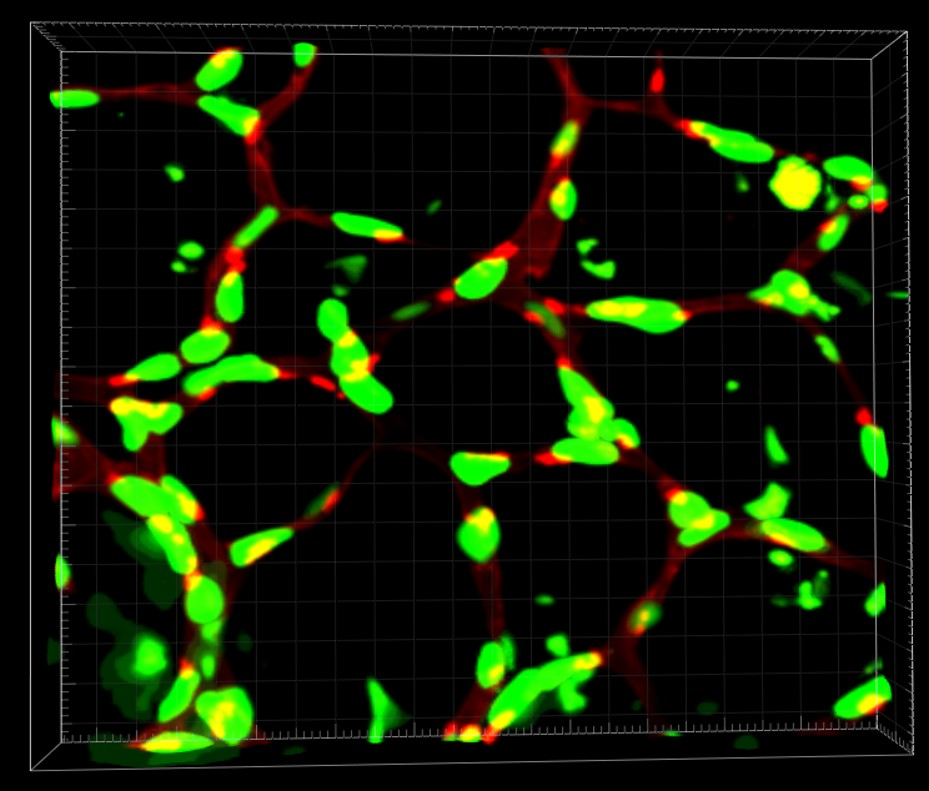
\includegraphics[width=3.5cm]{Images/pre_crop5_image.jpg}}\hfil 
\subfigure[]{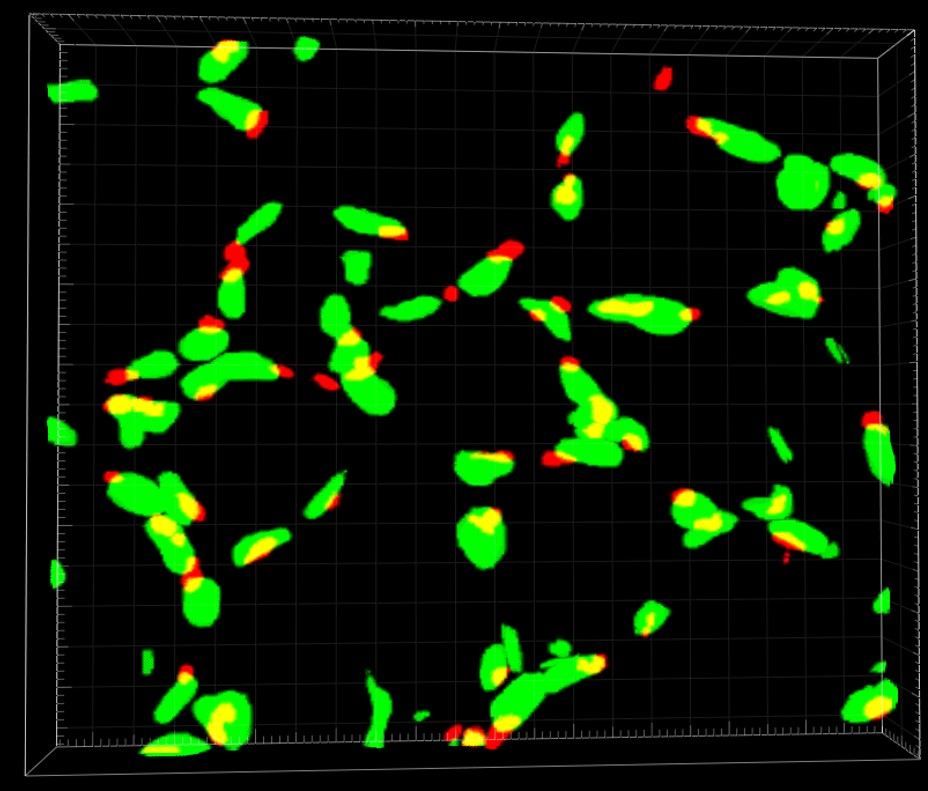
\includegraphics[width=3.5cm]{Images/2-mask-crop5.jpg}}\hfil
\subfigure[]{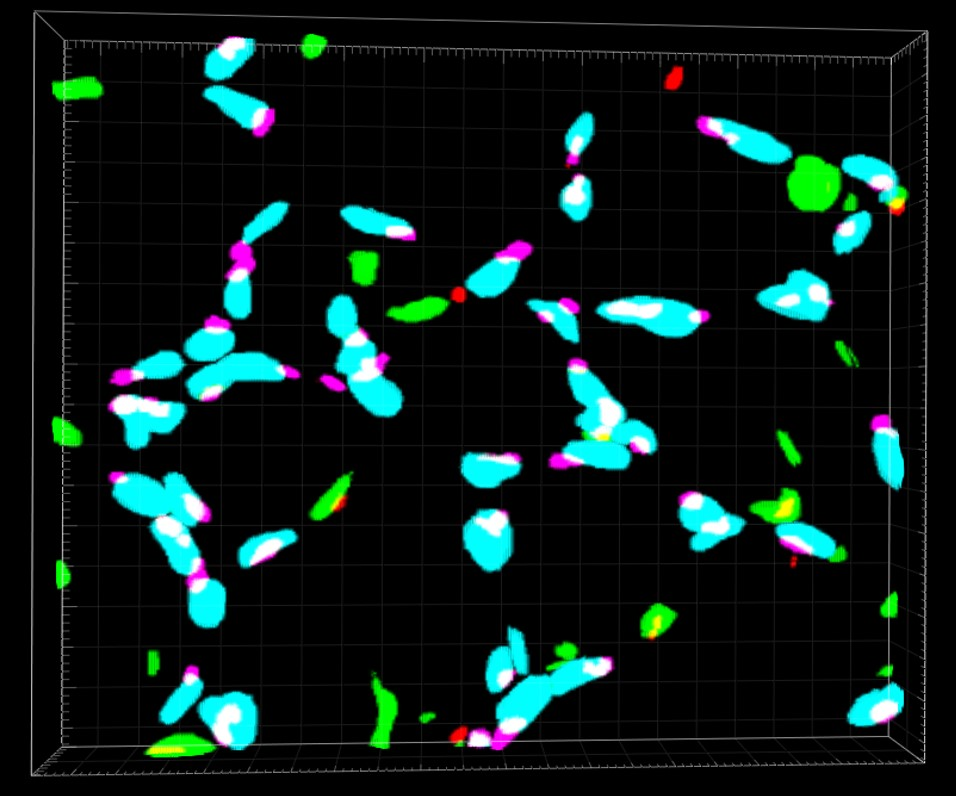
\includegraphics[width=3.5cm]{Images/3-mask-crop5-original.jpg}}

\subfigure[]{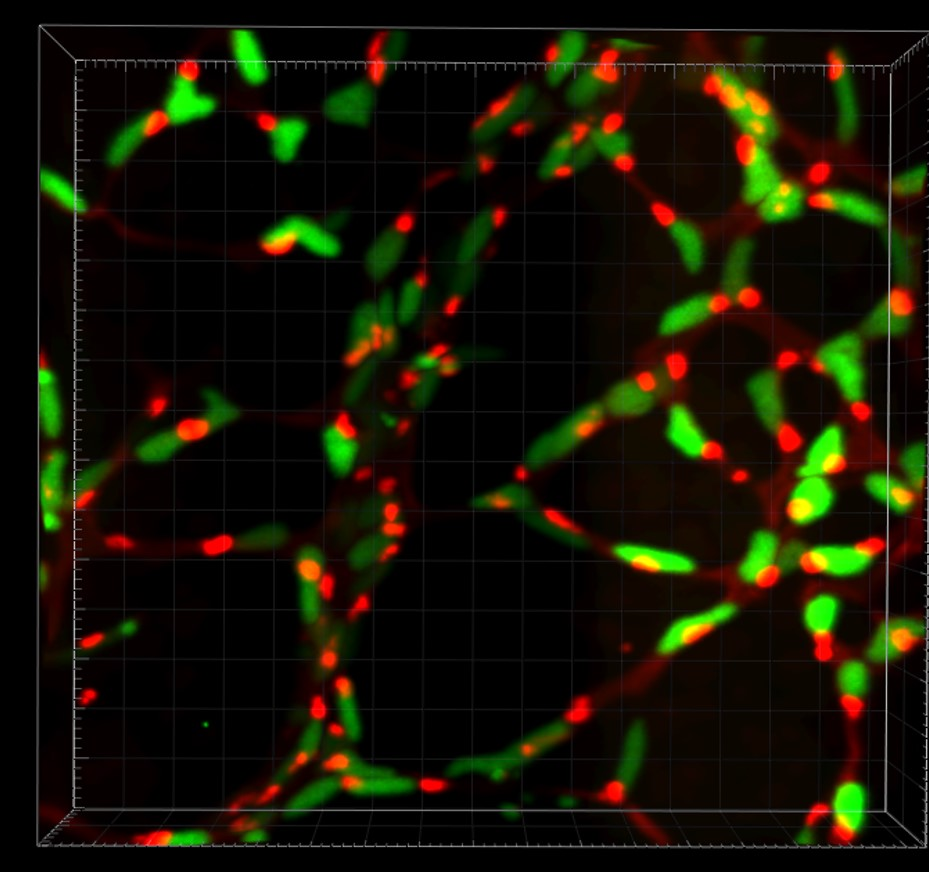
\includegraphics[width=3.5cm]{Images/crop7_img.jpg}}\hfil 
\subfigure[]{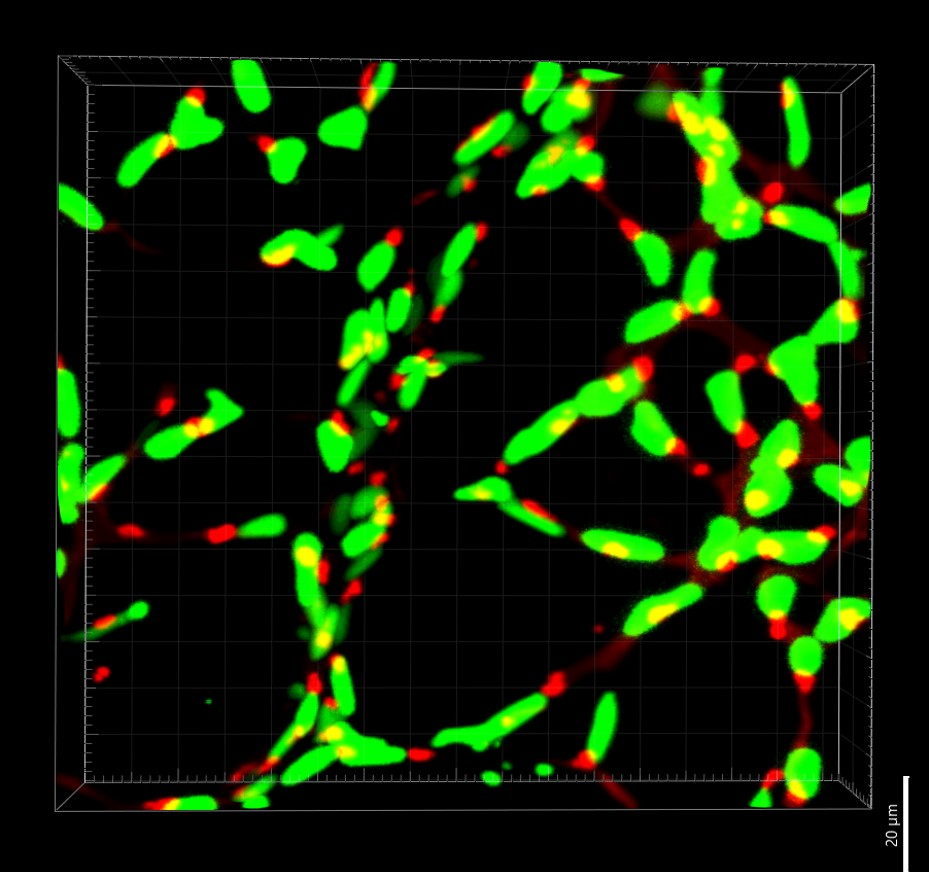
\includegraphics[width=3.5cm]{Images/pre_crop7_image.jpg}}\hfil
\subfigure[]{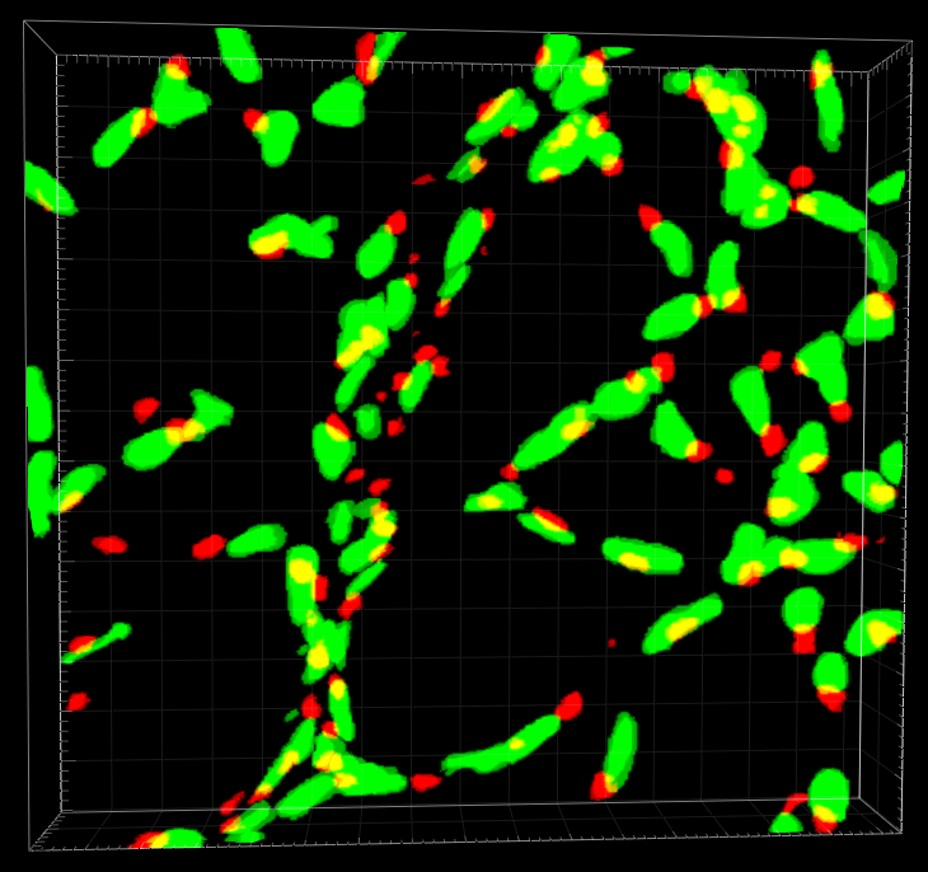
\includegraphics[width=3.5cm]{Images/2-mask-crop7.jpg}}\hfil
\subfigure[]{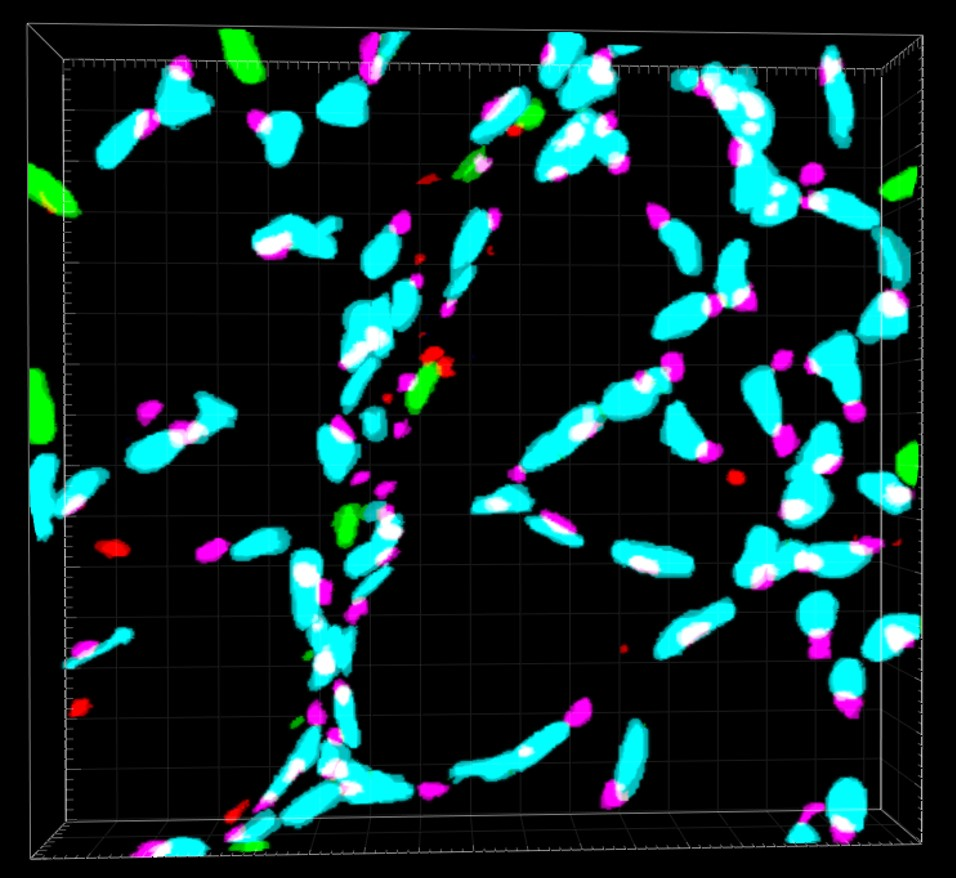
\includegraphics[width=3.5cm]{Images/3-mask-crop7-original.jpg}}
\caption{3D visualization of crops used for testing the models: (a) $I^{orig}_1$; (b) $I^{Pre}_1$; (c) $I^{gt}_{21}$; (d) $I^{gt}_{31}$; (e) $I^{orig}_2$; (f)  $I^{Pre}_2$; (g) $I^{gt}_{22}$; (h) $I^{gt}_{32}$.}

\label{fig:dataset}

\end{figure}

As mentioned in section \ref{section:dataset}, the crops for training the proposed models were divided into equal-sized patches. Therefore, the training dataset for all proposed models consists of 433 patches with a size of 64x64x64 from 6 different crops.

\subsection{3D U-Net}

In this subsection the results obtained by training and testing the 3D U-Net model are presented and discussed.

\subsubsection*{Implementation Details}

First, details on the choice of the model's hyperparameters are presented.

In all experiments, using the \ac{3D} U-Net model: Early stopping was applied to stop training when the validation loss did not improve for 10 epochs; the model was trained with the ADAM optimizer with a learning rate of 1e-3; using Xavier initialization for the model weights; a batch size of 4 and \ac{ReLU} as activation functions, except in the last layer, which has a sigmoid activation function so that the output is $n$-probability maps (where $n$ is the number of classes). A threshold of 0.5 is then applied to each probability map of the output of the U-Net to obtain the final segmentation mask.


\subsubsection*{2 Class}

The U-Net model was first trained with the original dataset (figure \ref{fig:micro}). The obtained segmentation masks for the experiment are shown in figures \ref{fig:results-unet} (b) and \ref{fig:results-unet} (e), and table \ref{tab:u-net-results} lists the values obtained for the metrics used to evaluate the model which were described in section \ref{section:metrics}.

From the results, it can be concluded that in the original dataset the precision of the nuclei and especially the Golgi is very low, which indicates over-segmentation and can be verified by looking at the obtained images. This also leads to a very low dice coefficient. Therefore, to improve these results, the pre-processing method described in the previous section \ref{section:pre} was applied to the microscopic images and the U-Net model was re-trained with patches extracted from the pre-processed images.

The segmentation masks obtained for the pre-processed microscopic images are shown in figures \ref{fig:results-unet} (c) and \ref{fig:results-unet} (f) and table \ref{tab:u-net-results} provides the values of the metrics used to evaluate the model. Compared to the previous results, the pre-processing method improved the results significantly, especially the precision and Dice Coefficient. However, it still tends to over-segment, especially the Golgi.

% Please add the following required packages to your document preamble:
% \usepackage{graphicx}
\begin{table}[!htb]
\centering
\caption{Average metric values after testing the 3D U-Net model on two microscopic images for a model trained with the original microscopic images (U-Net) and with the pre-processed microscopic images (U-Net + Pre)}
\label{tab:u-net-results}
\resizebox{\columnwidth}{!}{%
\renewcommand\arraystretch{1.4}
\begin{tabular}{c|c|c|c|c|c|c|}
\cline{2-7}
                                  & \multicolumn{1}{l|}{DC   Nuclei} & \multicolumn{1}{l|}{DC Golgi} & \multicolumn{1}{l|}{Precision Nuclei} & \multicolumn{1}{l|}{Precision Golgi} & \multicolumn{1}{l|}{Recall Nuclei} & \multicolumn{1}{l|}{Recall Golgi} \\ \hline
\multicolumn{1}{|c|}{U-Net}       & 0,4497                           & 0,3054                        & 0,2912                                & 0,1842                               & 0,9895                             & 0,9186                            \\ \hline
\multicolumn{1}{|l|}{U-Net + Pre} & 0,7775                           & 0,6938                        & 0,7067                                & 0,6500                               & 0,8692                             & 0,7683                            \\ \hline
\end{tabular}%
}
\end{table}

\begin{figure}[!htb]
  
\centering
\subfigure[]{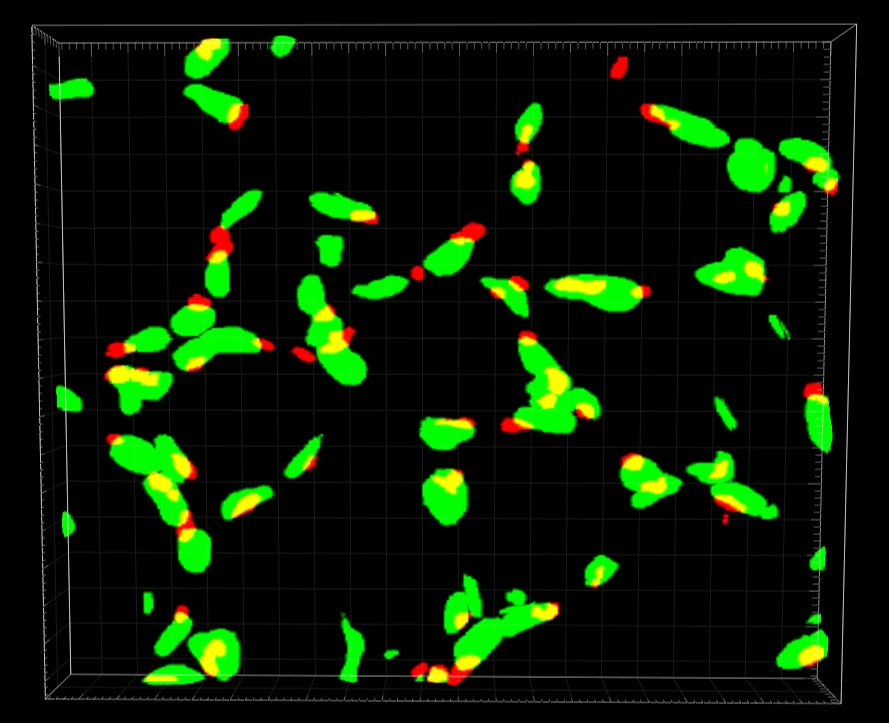
\includegraphics[width=4.5cm]{Images/mask-crop5.jpg}}\hfil
\subfigure[]{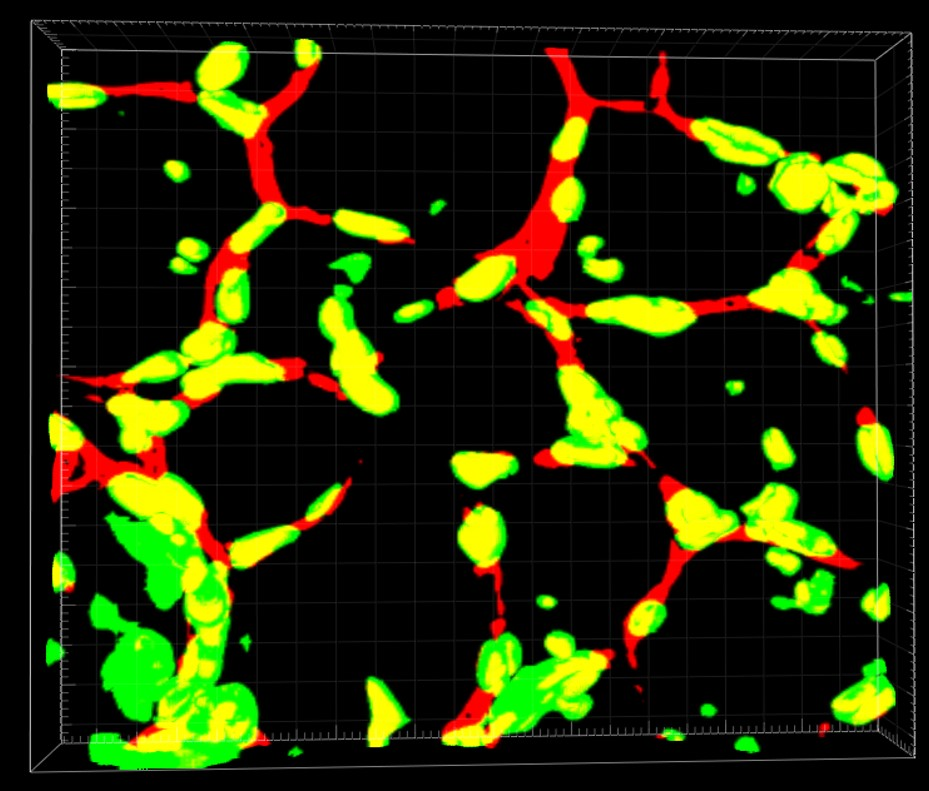
\includegraphics[width=4.5cm]{Images/u-net-crop5-not-pre.jpg}}\hfil 
\subfigure[]{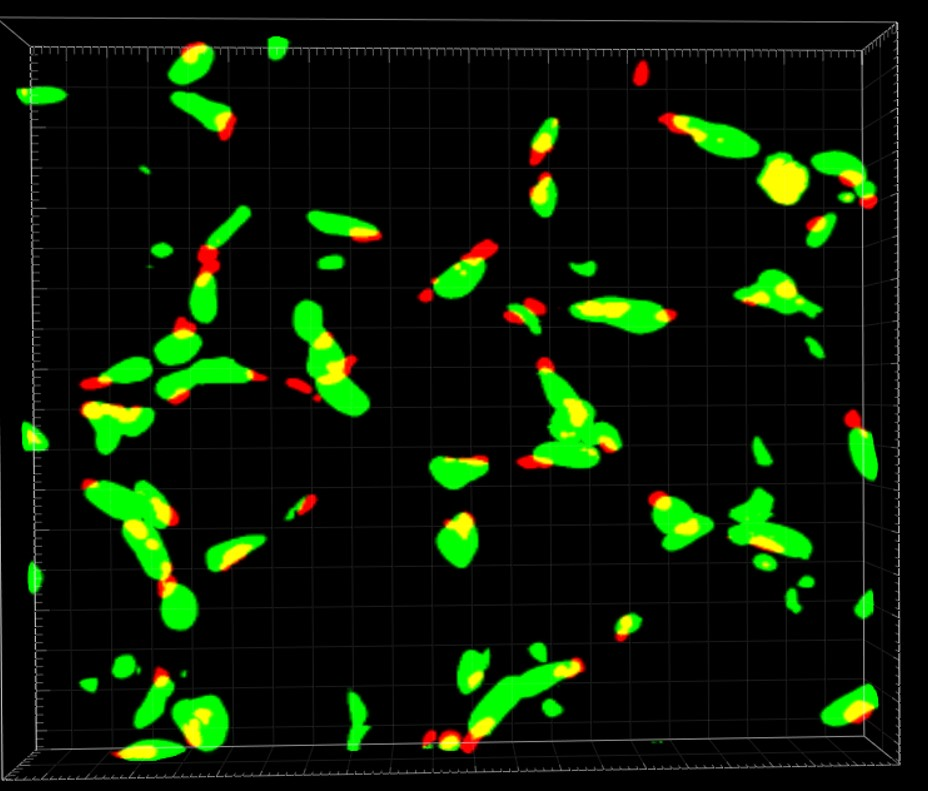
\includegraphics[width=4.5cm]{Images/u-net-aft-pre-crop5.jpg}} 

\subfigure[]{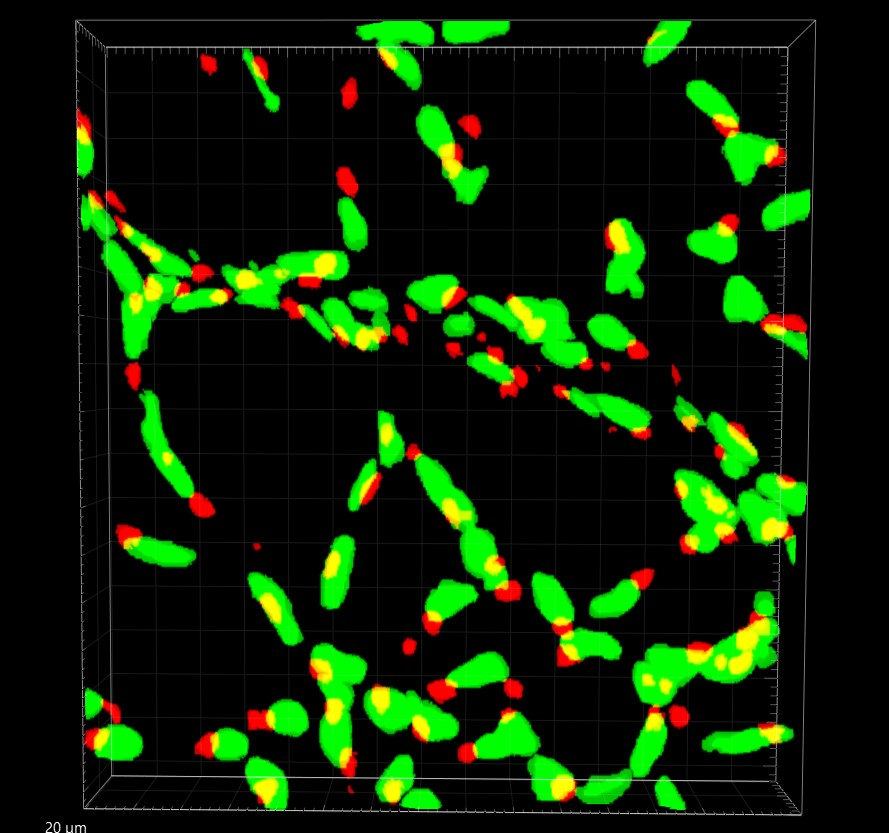
\includegraphics[width=4.5cm]{Images/mask-crop7.jpg}}\hfil 
\subfigure[]{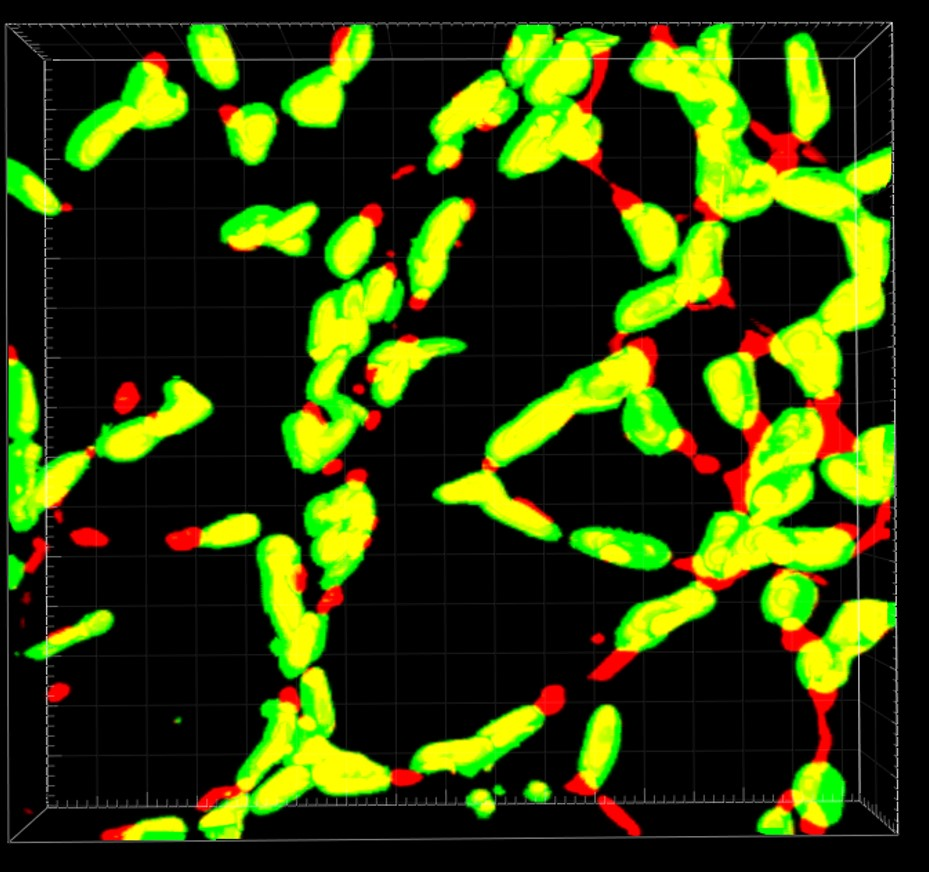
\includegraphics[width=4.5cm]{Images/u-net-crop7-not-pre.jpg}}\hfil
\subfigure[]{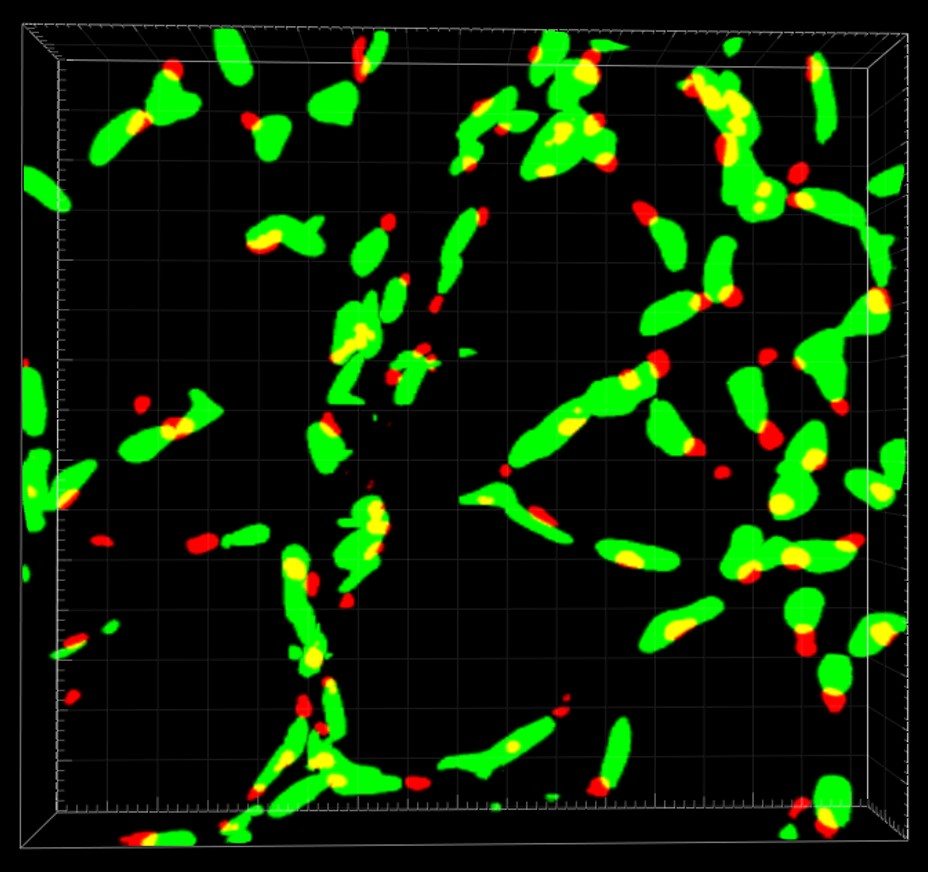
\includegraphics[width=4.5cm]{Images/u-net-aft-pre-crop7.jpg}}
\caption{3D visualization of segmentation masks: (a) 3D ground truth $I^{gt}_{21}$; (b) 3D U-Net model tested on $I^{orig}_1$; (c) 3D U-Net model tested on $I^{Pre}_1$; (d) 3D ground truth $I^{gt}_{22}$; (e) 3D U-Net model tested on $I^{orig}_2$; (f) 3D U-Net model tested on $I^{Pre}_2$.}

\label{fig:results-unet}

\end{figure}

There are two things that have been identified in the dataset that may lead to decreased precision of the model. The microscopic images have digital noise, which causes the model to classify this noise as Golgi/Nuclei. This has been verified specifically for the Golgi, and an example of this noise can be seen in figures \ref{fig:errors-unet} (d) to (f) highlighted by the blue circles. Another reason that leads to lower precision is that the manual segmentation masks contain annotation/segmentation errors. In figures \ref{fig:errors-unet} (a) to (c), we see that a Golgi is not identified in the segmentation mask  of our dataset, even though it is present in the microscopic image along with the nucleus and is identified correctly by the U-Net model.

The low recall can be explained by the fact that the microscopic images have low contrast in certain areas, even after applying the pre-processing method to the images. This causes the model to fail to recognise some Golgi/nuclei, which lowers the recall. This case is illustrated in figure \ref{fig:errors-unet} (d) to (e) by the orange circle.

\begin{figure}[!htb]

\centering
\subfigure[]{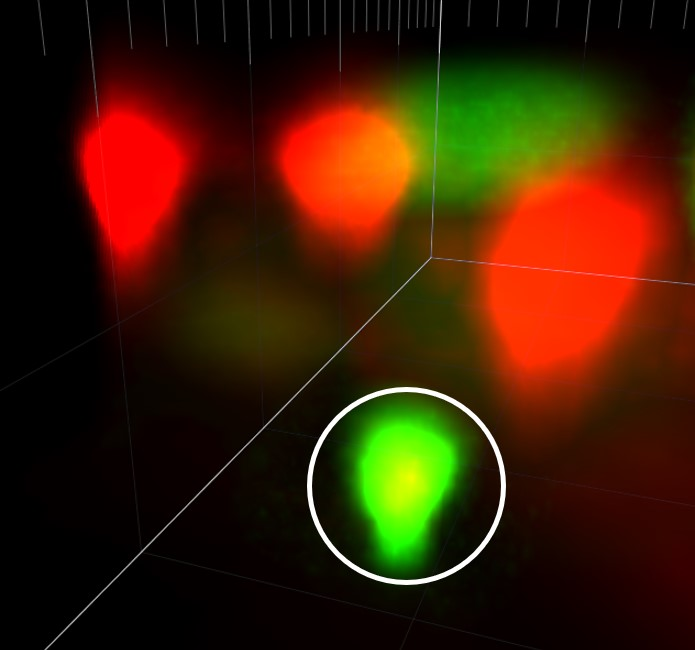
\includegraphics[width=4cm]{Images/image_noise.jpg}}\hfil
\subfigure[]{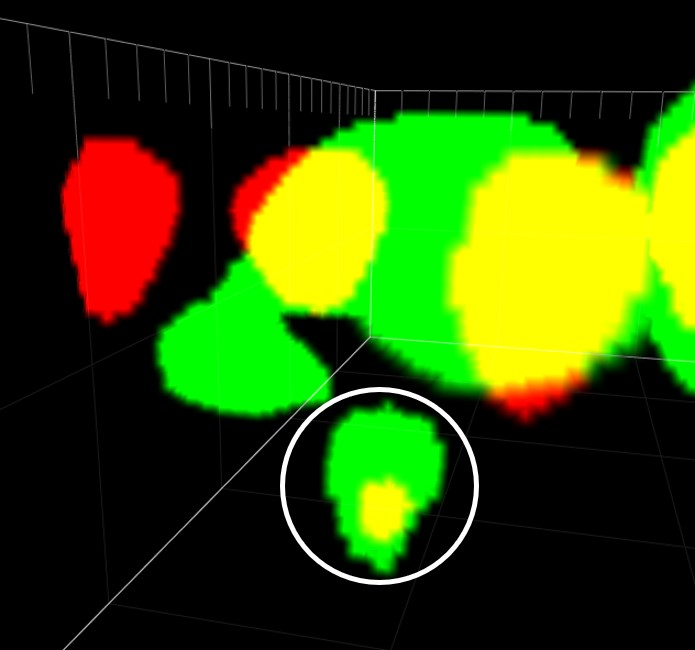
\includegraphics[width=4cm]{Images/my_mask_noise.jpg}}\hfil 
\subfigure[]{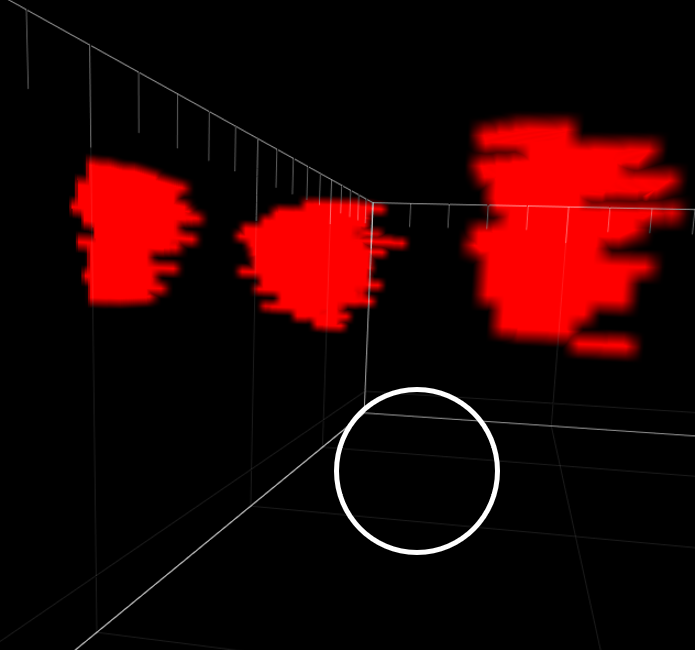
\includegraphics[width=4cm]{Images/real_mask_noise.jpg}} 

\subfigure[]{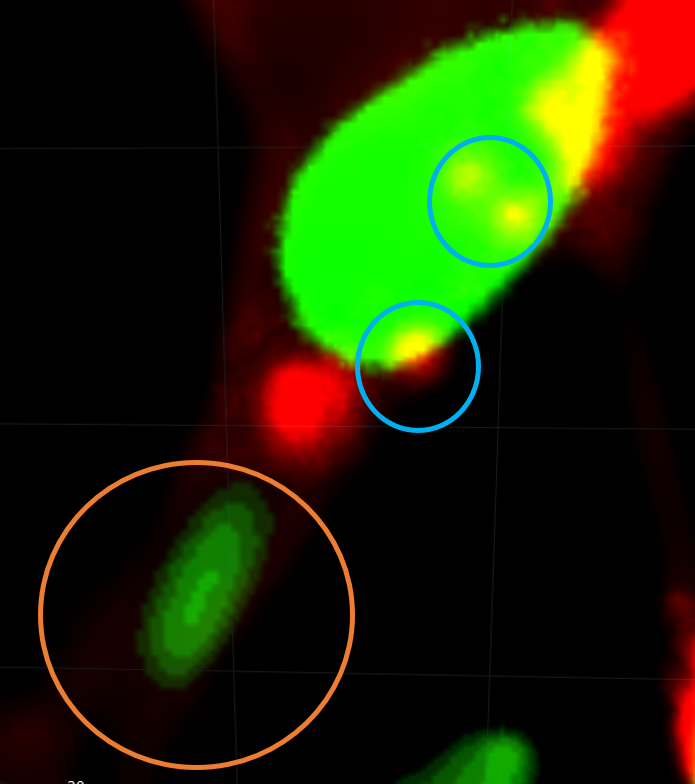
\includegraphics[width=4cm]{Images/noise_recall_image.jpg}}\hfil   
\subfigure[]{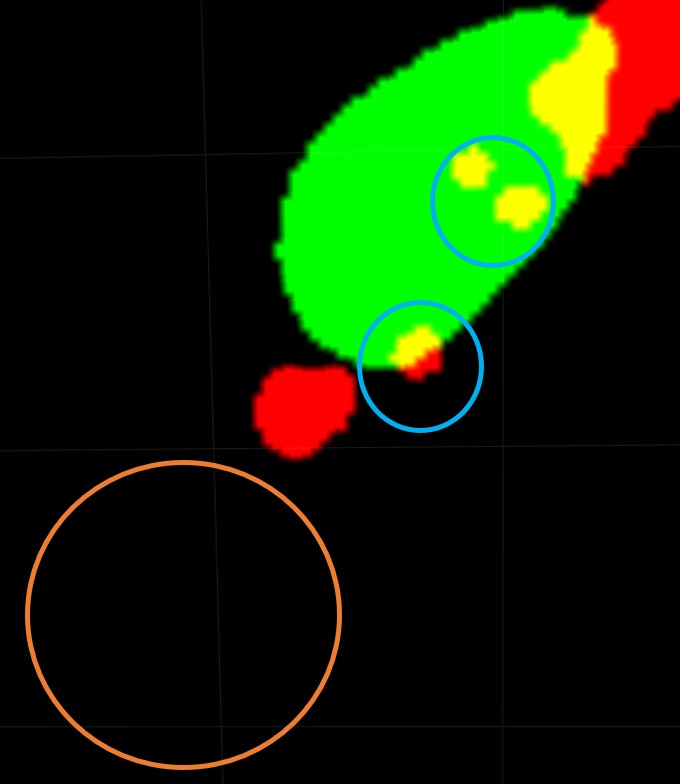
\includegraphics[width=4cm]{Images/noise_recall_my_mask.jpg}}\hfil
\subfigure[]{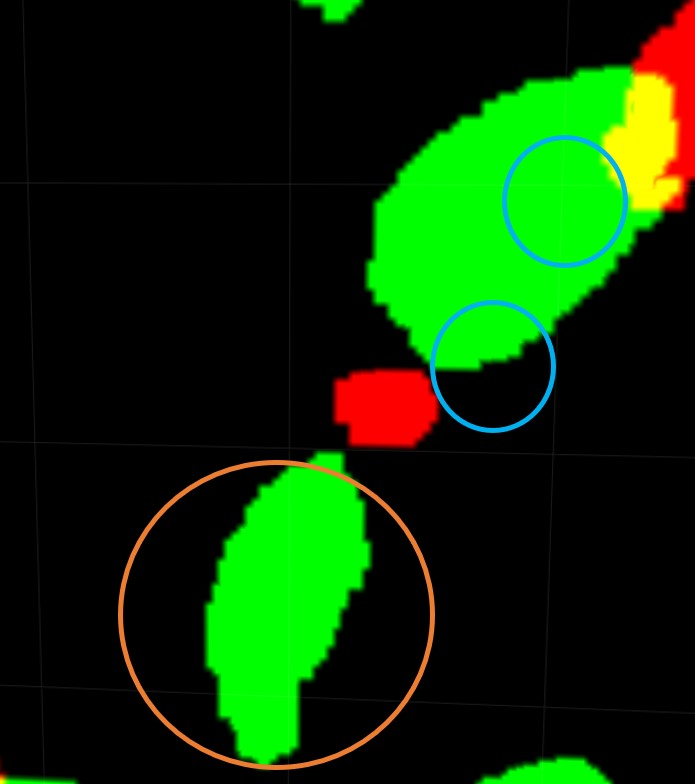
\includegraphics[width=4cm]{Images/noise_recall_real_mask.jpg}}
\caption{Example of ground truth mask imperfection highlighted by white circle; Example of digital noise highlighted by blue circles; and example of nondetection by 3D U-Net model highlighted by orange circle; (a) and (d) 3D microscopic section; (b) and (e) 3D U-Net segmentation mask; (c) and (f) 3D ground truth segmentation mask.}
\label{fig:errors-unet}



\end{figure}

To improve the results, different loss functions were tried to better segment the nuclei and Golgi, which would account for the imbalance between the background and the nuclei/Golgi, for example Focal Loss \cite{focal_loss}, but this did not lead to better results, instead caused the model to detect more noise. Another attempt was made by increasing the size of the data by applying transformations such as rotations and flips (reflections) to patches of the pre-processed dataset, but again this also did not produce better results but resulted in the model detecting more noise.

\subsubsection*{3 Class}

In this approach, the number of output probability maps of the 3D U-Net is three, so we can classify the nuclei, Golgi and nucleus-Golgi pairs of the input images. All other parameters described in the implementation details are kept. The model is trained with the pre-processed dataset and respective ground truth masks.

After training, the performance of the model is tested with the two microscopic image volumes $I^{Pre}_1$ and $I^{Pre}_2$. Figure \ref{fig:results-unet-3channel} is a 3D visualization of the segmentation results for these volumes and table \ref{tab:results-3class-u-net} shows the average quantitative results.

\begin{figure}[!htb]
\centering
\subfigure[]{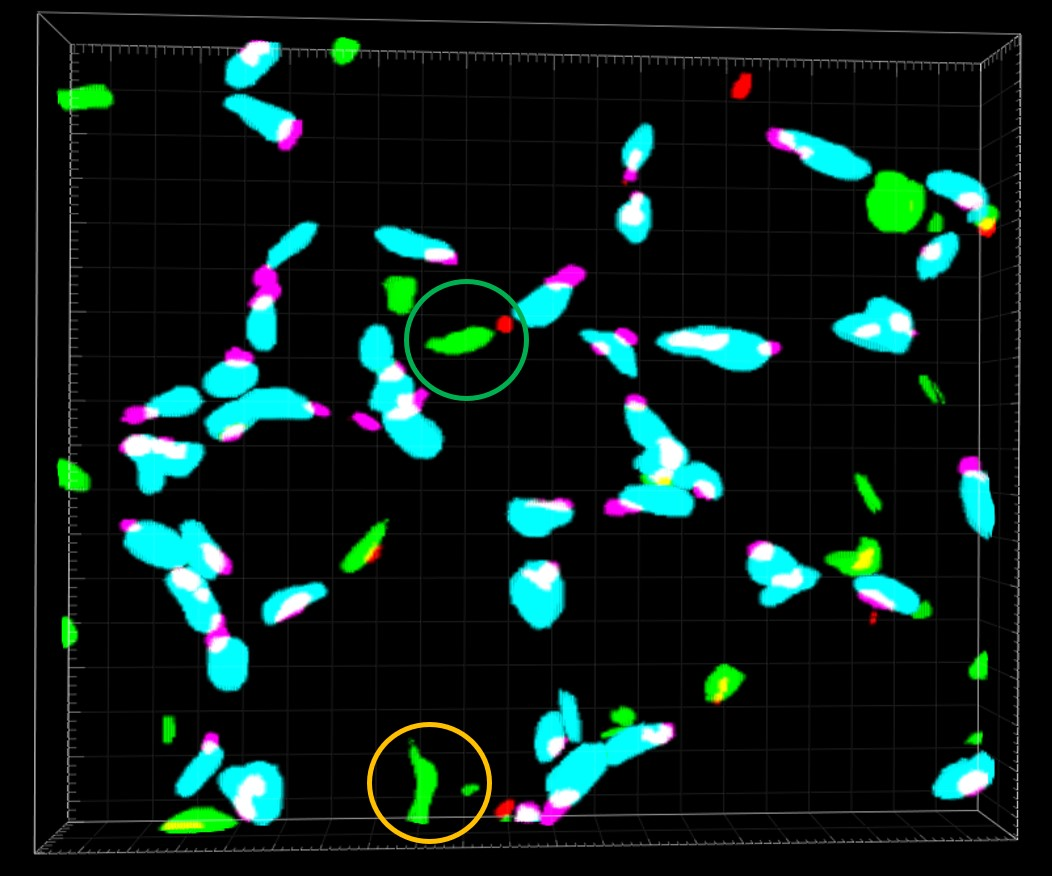
\includegraphics[width=5cm]{Images/3-mask-crop5.jpg}}\hfil
\subfigure[]{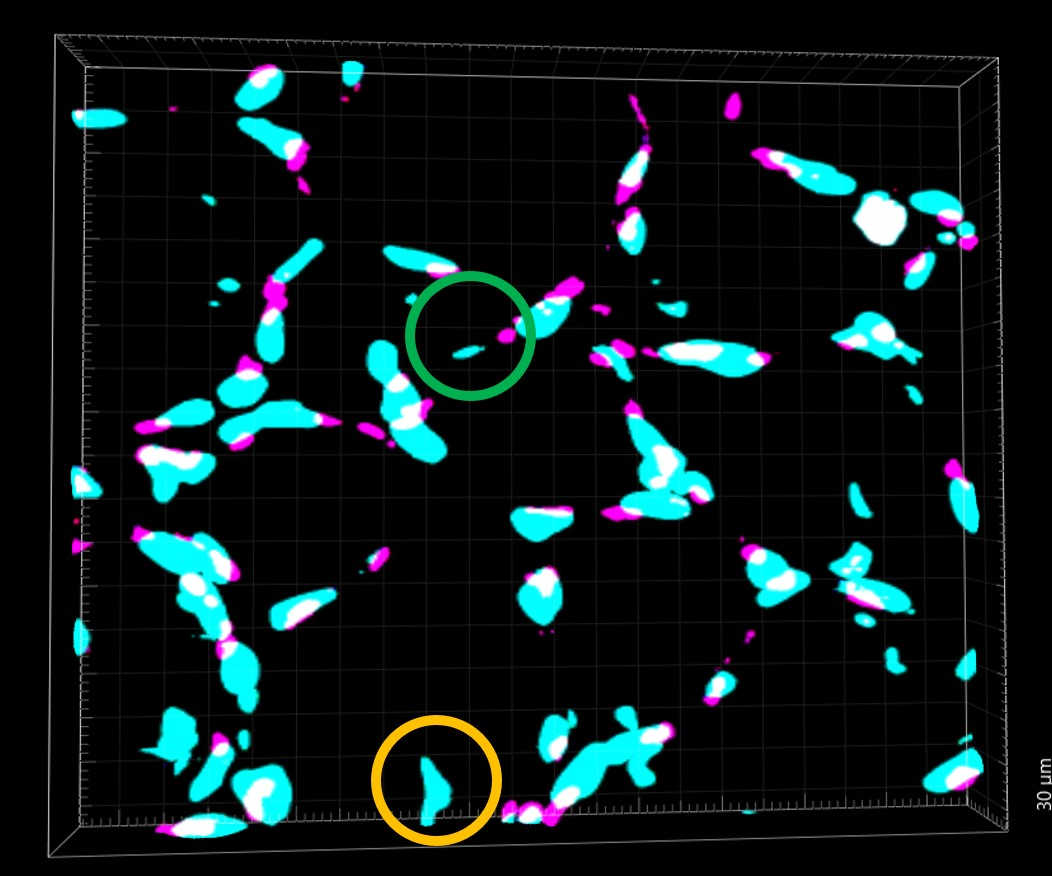
\includegraphics[width=5cm]{Images/u-net-3class-crop5.jpg}}

\subfigure[]{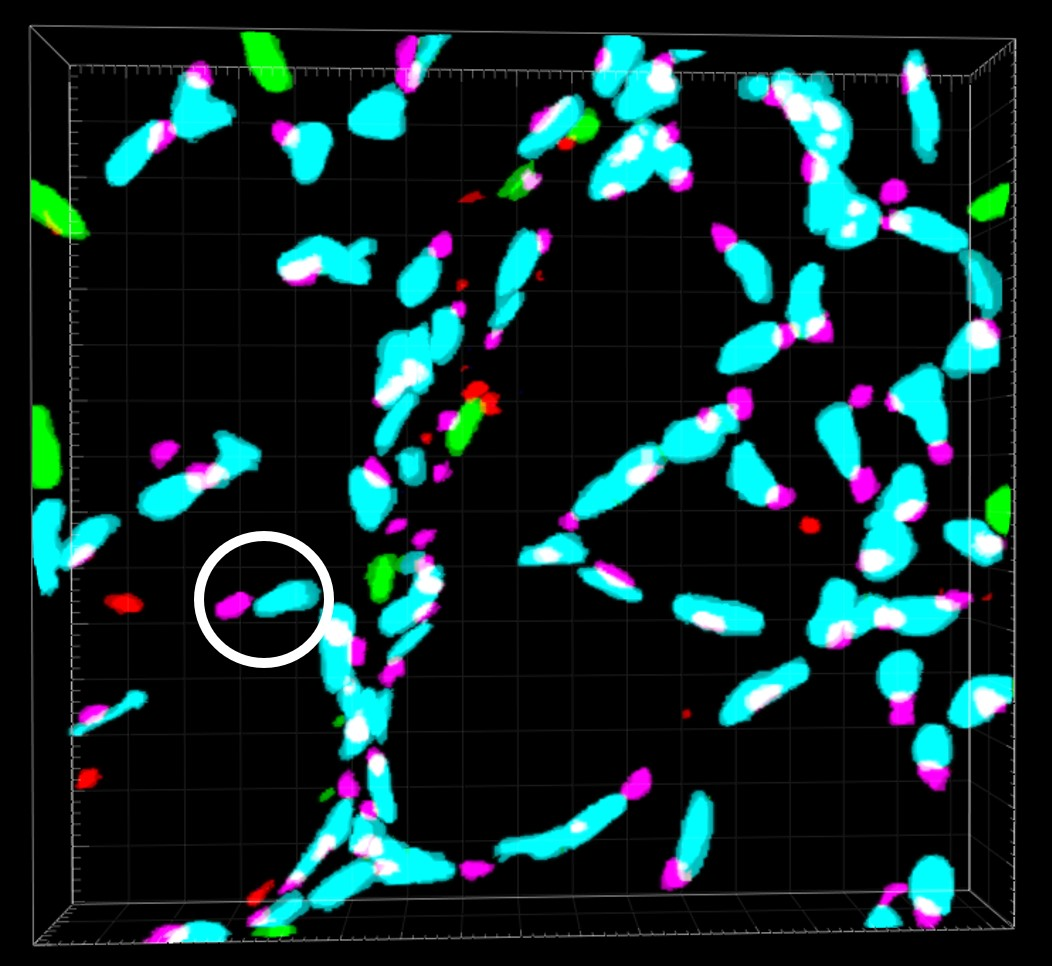
\includegraphics[width=5cm]{Images/3-mask-crop7.jpg}}\hfil 
\subfigure[]{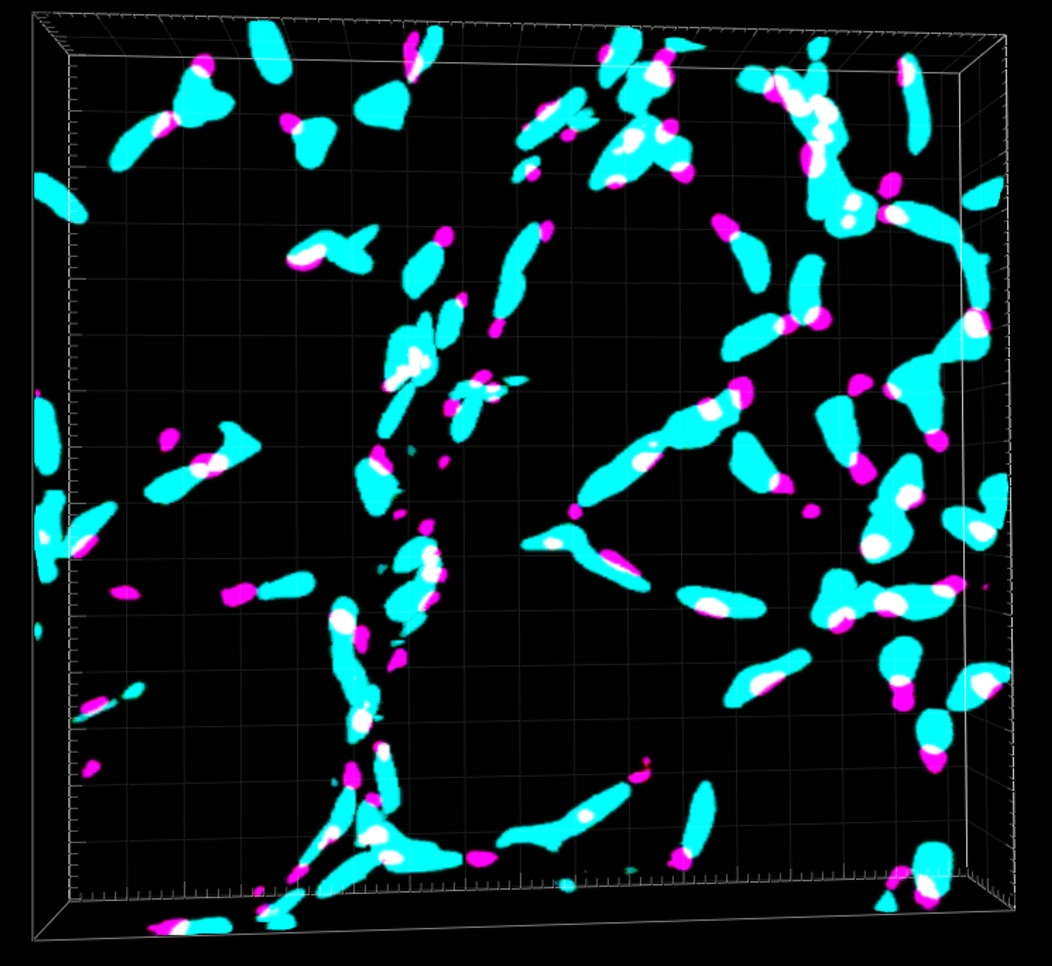
\includegraphics[width=5cm]{Images/u-net-3class-crop7.jpg}}

\caption{3D visualization of segmentation masks: (a) 3D ground truth $I^{gt}_{31}$; (b) 3 class 3D U-Net model tested on $I^{Pre}_1$; (c) 3D ground truth $I^{gt}_{32}$; (d) 3 class 3D U-Net model tested on $I^{Pre}_2$.}

\label{fig:results-unet-3channel}

\end{figure}

% Please add the following required packages to your document preamble:
% \usepackage{graphicx}
\begin{table}[!htb]
\centering
\caption{Average metric values after testing the 3 class 3D U-Net model on two pre-processed microscopic images}
\label{tab:results-3class-u-net}
\resizebox{\columnwidth}{!}{%
\renewcommand\arraystretch{1.4}
\begin{tabular}{|c|c|c|c|c|c|c|c|c|}
\hline
DC Nuclei & DC Golgi & DC Pair & Precision Nuclei & Precision Golgi & Precision Pair & Recall Nuclei & Recall Golgi & Recall Pair \\ \hline
0,7916    & 0,6752   & 0,7601  & 0,7589           & 0,5935          & 0,6941         & 0,8278        & 0,8206       & 0,8403      \\ \hline
\end{tabular}%
}
\end{table}

From Table \ref{tab:results-3class-u-net} we can see that, as expected, the Dice Coefficient, precision, and recall for the nuclei and Golgi classes are comparable to the values obtained previously. Looking at the results for the nucleus-Golgi pairs class, we can see from the segmentation masks in figure \ref{fig:results-unet-3channel} that the model is generally able to correctly identify this class, as reflected by a recall of 0.8403. However, the yellow circles in figure \ref{fig:results-unet-3channel} mark cases where the model is apparently unable to distinguish that an isolated nucleus or Golgi are not part of a pair and therefore should not be identified in the segmentation mask for the nucleus-Golgi pairs. Therefore, it also detects a lot of digital noise, which is reflected in the lower precision of 0.6941. The reason the model cannot learn these cases could be that these cases of isolated nuclei and Golgi are relatively rare and do not occur often enough in the dataset for the model to distinguish them.

As mentioned above, the ground truth mask for the Golgi and the nuclei has some imperfections. The main one is the fact that in the cases where the nuclei and the Golgi pairs do not overlap, no connection is made between them, which makes it difficult for the model to distinguish, for example, an isolated Golgi from a paired one. An example of this case is highlighted by the white circle in figure \ref{fig:results-unet-3channel}. Additionally, some of the nucleus-Golgi pairs are not annotated in the ground truth masks, but are correctly identified by the model, which also affects the precision results for the nucleus-Golgi pairs class. An example of this case is highlighted by a green circle in figure \ref{fig:results-unet-3channel}.

\subsection{Vox2Vox}

In this subsection the results obtained by training and testing the Vox2Vox model are presented and discussed.

\subsubsection*{Implementation Details}

As mentioned earlier, the Vox2Vox model consists of two networks, a generator and a discriminator. The discriminator is used only to improve the training, the generator is the segmentation network we want to obtain. In these two networks, the following specifications were set for training: He normal initialization for the model weights; the Adam Optimizer with a learning rate of 2e-5; batch size of 4 and early stopping to stop training when the validation loss did not improve for 20 epochs, saving the weights of the best model based on the lowest validation loss.

Specifically for the Vox2Vox generator, the sigmoid activation function was used in the last layer so that the output has $n$-probability maps (where $n$ is the number of classes). A threshold of 0.5 is then applied to each probability map of the output of Vox2Vox to obtain the final segmentation mask volume. The hyper-parameter $\alpha$ from the generator loss defined previously in equation \ref{eq:vox2vox-generator-loss} is set to $\alpha = 5$ as proposed in \cite{vox2vox}.

In a first phase, the model was trained with a loss function for the generator that gave the same weight to the nuclei and Golgi. However, with this loss function, the model had great difficulty detecting the Golgi on the images. This is likely due to the fact that many of the patches used to train the model do not contain Golgi, making it difficult for the model to learn how to detect and segment this class. To improve the results, the loss function of the generator was modified to give more weight to the Golgi dice coefficient loss. The term \ac{DLoss} in the equation \ref{eq:vox2vox-generator-loss} was changed to

\begin{equation}
    DLoss_{total} = \beta_1 DLoss(y_N,\hat{y}_N) + \beta_2 DLoss(y_G,\hat{y}_G)
\end{equation}

\noindent where $y_N$ and $y_G$ are the ground truth segmentation masks of nuclei and Golgi, respectively, and $\hat{y}_N$ and $\hat{y}_G$ are the predicted segmentation masks of nuclei and Golgi, respectively. We found the most appropriate values for $\beta_1$ and $\beta_2$ by trial and error, and after some experiments, we set $\beta_1 = 1$ and $\beta_2 = 6$.


\subsubsection*{2 Class}

The Vox2Vox model was trained with the pre-processed dataset and tested with the two microscopic image volumes $I^{Pre}_1$ and $I^{Pre}_2$. Figure \ref{fig:results-vox2vox-2channel} is a 3D visualization of the segmentation results for these volumes and table \ref{tab:results-2class-vox2vox} shows the average quantitative metrics. 

% Please add the following required packages to your document preamble:
% \usepackage{graphicx}
\begin{table}[!htb]
\centering
\caption{Average metric values obtained from testing the 2 class Vox2Vox model on two pre-processed microscopic images}
\label{tab:results-2class-vox2vox}
\renewcommand\arraystretch{1.4}
\begin{tabular}{|c|c|c|c|c|c|}
\hline
DC  Nuclei & DC Golgi & Precision Nuclei & Precision Golgi & Recall Nuclei & Recall Golgi \\ \hline
0,7539     & 0,6883   & 0,6529           & 0,7078          & 0,8933        & 0,6917       \\ \hline
\end{tabular}%

\end{table}

\begin{figure}[!htb]
\centering
\subfigure[]{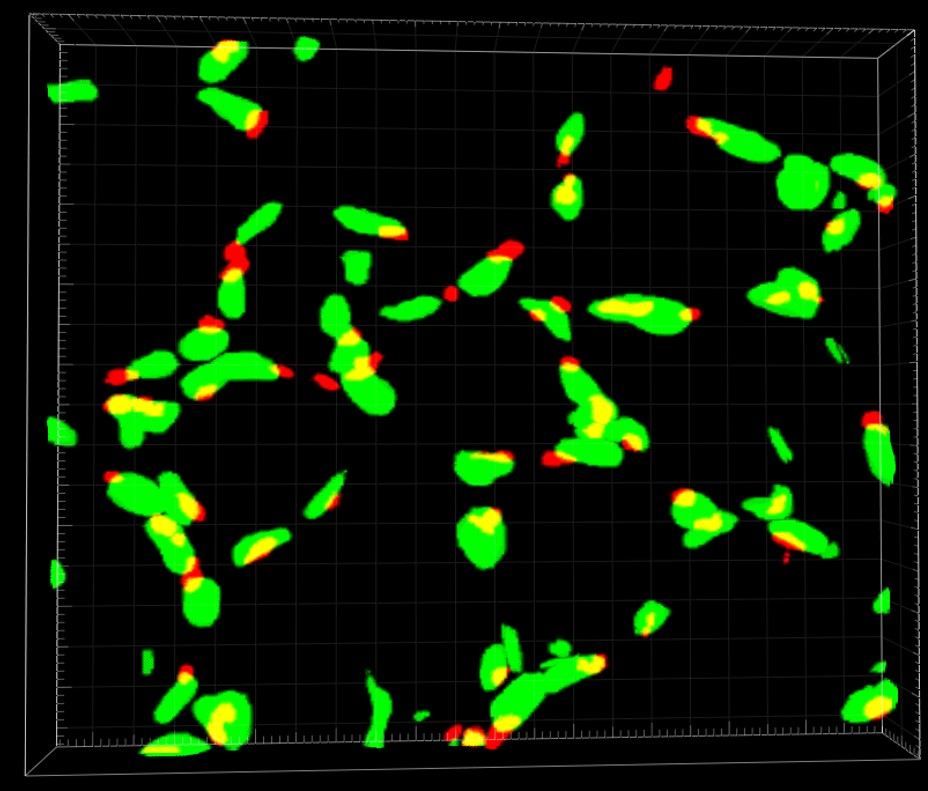
\includegraphics[width=5cm]{Images/2-mask-crop5.jpg}}\hfil
\subfigure[]{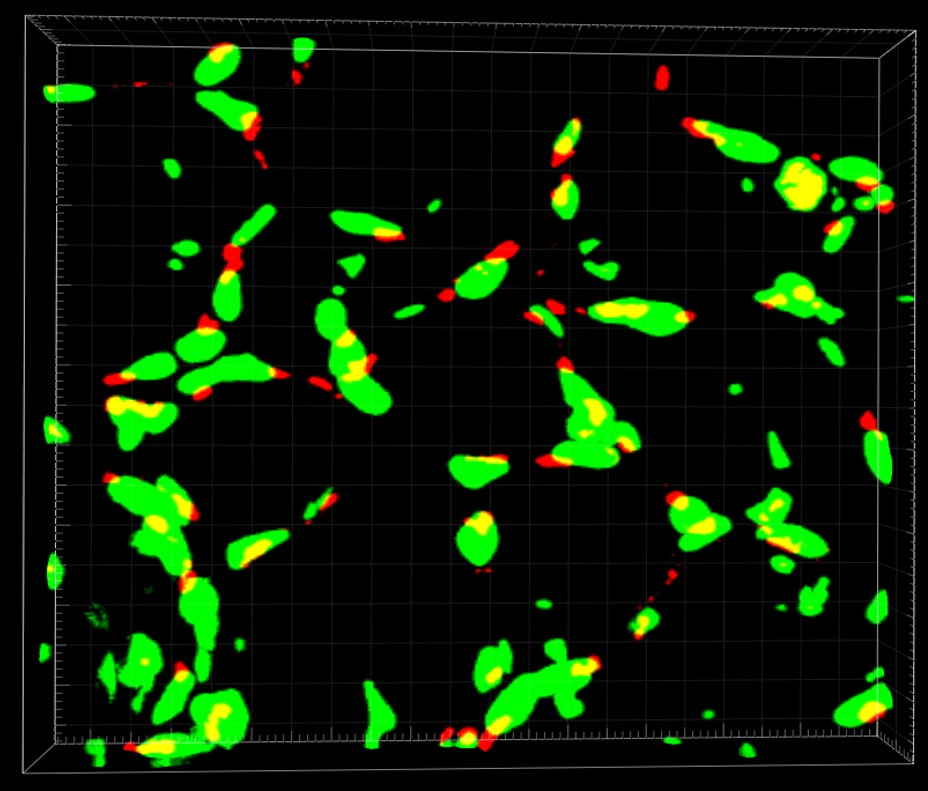
\includegraphics[width=5cm]{Images/vox2vox-2class-crop5.jpg}}

\subfigure[]{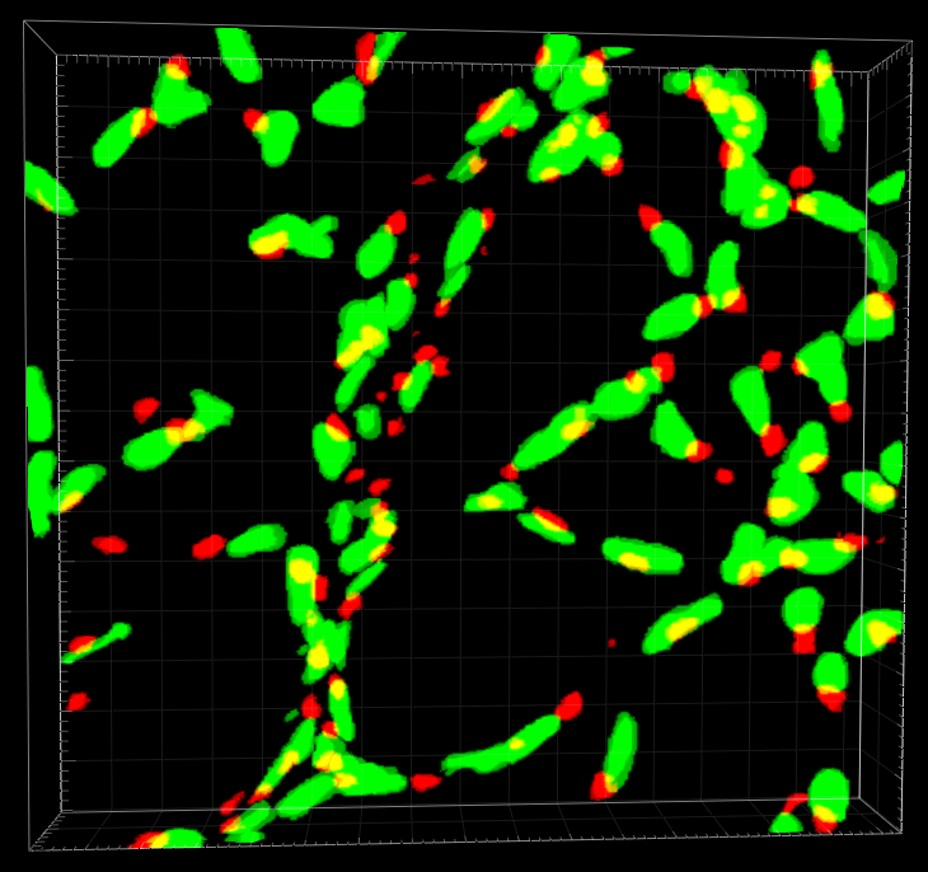
\includegraphics[width=5cm]{Images/2-mask-crop7.jpg}}\hfil 
\subfigure[]{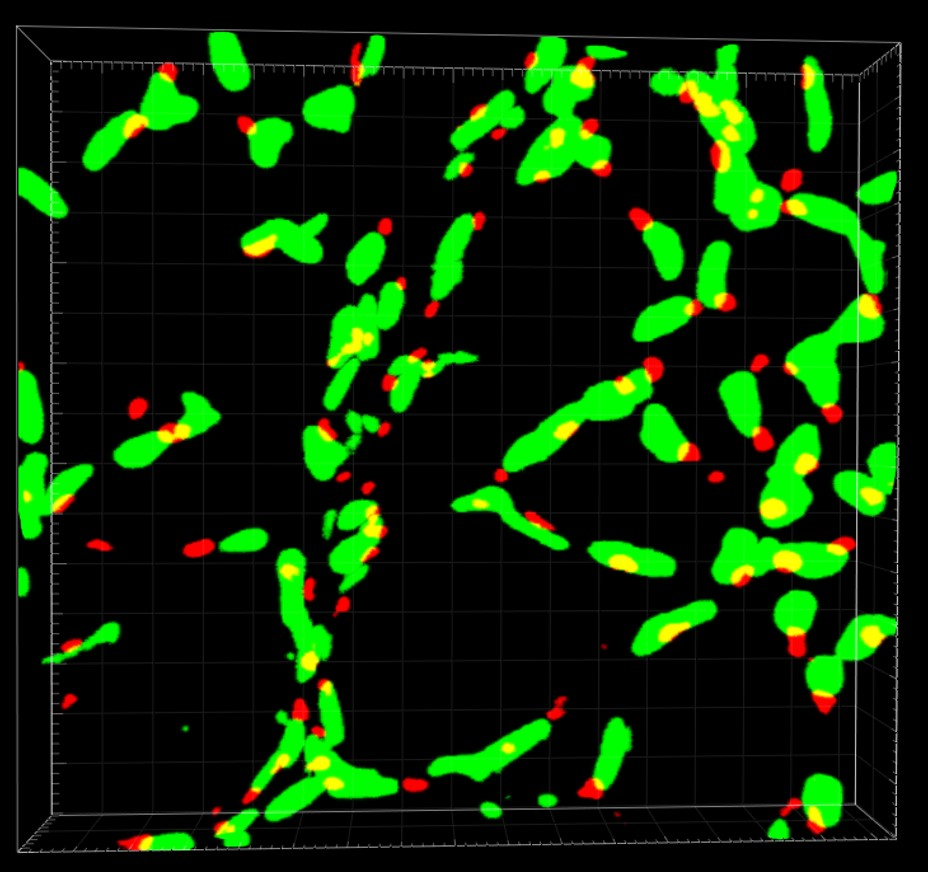
\includegraphics[width=5cm]{Images/vox2vox-2class-crop7.jpg}}

\caption{3D visualization of segmentation masks: (a) 3D ground truth $I^{gt}_{21}$; (b) 2 class Vox2Vox model tested on $I^{Pre}_1$; (c) 3D ground truth $I^{gt}_{22}$; (d) 2 class Vox2Vox model tested on $I^{Pre}_2$.}

\label{fig:results-vox2vox-2channel}

\end{figure}

From the results for the dice coefficient, we can conclude that the model is successful in identifying most of the nuclei and Golgi in the microscopic image volumes. For the Golgi segmentation mask, we verified in figure \ref{fig:results-vox2vox-2channel} that the model correctly identifies all Golgi. However, the margins for all Golgi are smaller than the ground truth segmentation mask, resulting in lower recall. This is likely due to the fact that the ground truth segmentation masks have low resolution, as shown in Figure \ref{fig:errors-unet} (c), and also to discontinuities in \ac{3D}, since these masks are created slide by slide in 2D. Consequently, the Vox2Vox model learns to generate images with this low resolution, which makes it difficult to segment the margins, especially of small objects like Golgi.

For the cell nuclei, we found that the model is very sensitive to noise in this class. This is particularly evident in the $I^{Pre}_1$ image test, as part of this image contains a lot of background noise for the nucleus channel and this noise is detected by the model, resulting in lower precision. However, this also results in the model being able to detect Golgi that are difficult to classify, i.e., Golgi with low contrast in the segmentation mask.


\subsubsection*{3 Class}

In this method, the number of output probability maps of Vox2Vox generator model is three, so we can classify the nuclei, Golgi and nucleus-Golgi pairs of the input images. All other parameters described in the implementation details are retained, except for the generator loss function, where we add another term to account for the Dice Loss of the nucleus-Golgi pairs class and set a gain $\beta_3$ = 1. The model was then trained using the pre-processed dataset and respective ground truth masks.

After training, the performance of the model is tested on the two microscopic image volumes $I^{Pre}_1$ and $I^{Pre}_2$. Figure \ref{fig:results-vox2vox-3channel} is a 3D visualization of the segmentation results for these volumes and table \ref{tab:results-3class-vox2vox} shows the average quantitative results.

\begin{table}[!htb]
\centering
\caption{Average metric values obtained from testing the 3 class Vox2Vox model on two pre-processed microscopic images}
\label{tab:results-3class-vox2vox}
\resizebox{\columnwidth}{!}{%
\renewcommand\arraystretch{1.4}
\begin{tabular}{|c|c|c|c|c|c|c|c|c|}
\hline
DC Nuclei & DC Golgi & DC Pair & Precision Nuclei & Precision Golgi & Precision Pair & Recall Nuclei & Recall Golgi & Recall Pair \\ \hline
0,7464    & 0,6720    & 0,7198 & 0,7170          & 0,6596          & 0,6763         & 0,7784        & 0,7204     & 0,7721      \\ \hline
\end{tabular}%
}
\end{table}

\begin{figure}[!htb]
\centering
\subfigure[]{\includegraphics[width=5cm]{Images/3-mask-crop5-original.jpg}}\hfil
\subfigure[]{\includegraphics[width=5cm]{Images/vox2vox-3class-crop5.jpg}}

\subfigure[]{\includegraphics[width=5cm]{Images/3-mask-crop7-original.jpg}}\hfil 
\subfigure[]{\includegraphics[width=5cm]{Images/vox2vox-3class-crop7.jpg}}

\caption{3D visualization of segmentation masks: (a) 3D ground truth $I^{gt}_{31}$; (b) 3 class Vox2Vox model tested on $I^{Pre}_1$; (c) 3D ground truth $I^{gt}_{32}$; (d) 3 class Vox2Vox model tested on $I^{Pre}_2$.}

\label{fig:results-vox2vox-3channel}

\end{figure}

If we compare the results presented in table \ref{tab:results-2class-vox2vox} and \ref{tab:results-3class-vox2vox} for the nuclei and Golgi classes, we verify that they remain relatively the same, as expected. Now, regarding the nucleus-Golgi pairs class, although the model is able to detect most of the nucleus-Golgi pairs in the images, the problem previously verified for the U-Net model remains in the Vox2Vox model, i.e., the model is not able to distinguish nucleus-Golgi pairs from individual nuclei and Golgi, which translates into lower precision. 

In figure \ref{fig:results-vox2vox-3channel} (d), it is highlighted by yellow circles that for this class, the model has difficulty segmenting small objects such as Golgi, which lowers the recall. This is also related to the fact that the ground truth segmentation masks have low resolution and the model learns to generate low resolution images as well.


\subsection{Proposed Approach - CycleGAN}

In this subsection the results obtained by training and testing the proposed unsupervised approach model CycleGAN are presented and discussed.

\subsubsection*{Implementation Details}

As mentioned in section \ref{section:proposed}, the CycleGAN model consists of four interconnected networks, two generators and two discriminators. After training, we keep only the generator corresponding to the segmentation network ($G_S$), the rest of the networks are used only to improve training. 

For training the CycleGAN we used: an initializer that generates weights with a normal distribution; the ADAM optimizer with a learning rate of 1e-3 and 5e-3 for the generators and discriminators, respectively; $\lambda_{cyc} = 10$ and $\lambda_{id} = 5$ in equation \ref{eq:total-cyclegan-loss} as proposed in \cite{cycleGAN:original} and a batch size of 2.

Specifically for the generators, the activation function \ac{Tanh} was used in the last layer so that the output has $n$-probability maps (where $n$ is the number of classes). Therefore, for these experiments, the input images had to be normalized to be in the range [-1,1]. Then the output images are normalized again to a range between [0,1]. For the segmentation network output ($G_S$), a threshold of 0.5 is then applied to each probability map to obtain the final segmentation mask volume.

During training, the performance of the model is tracked by using the generator models to generate translated versions of a few randomly selected images at the end of each epoch. The model is stopped when it reaches collapse mode, i.e., when it produces exactly the same output image for different input images. After training, we visually analyse the results obtained by CycleGAN for different epochs and select the model from the epoch that gives better results for the validation dataset.

Similar to Vox2Vox, we first trained the CycleGAN model by giving the Golgi and nuclei classes the same weight in the loss function. However, during training, we found that the model collapsed for the Golgi channel very quickly before it had a chance to improve. Therefore, similar to the Vox2Vox model, we changed the cycle consistency and identity loss to give more weight to the mean absolute error for Golgi. After some experiments the final weight given to this class was 3.5 and 1 to the nuclei class.


\subsubsection*{2 Class}

The CycleGAN was trained in two different ways: first in a supervised manner using the pre-processed microscopic image dataset together with the corresponding manually labelled segmentation masks to ensure the correct implementation of the model, and then in an unsupervised way with the synthetic segmentation mask dataset described in subsection \ref{subsection:synthetic_masks}. Then, both models were tested with the two microscopic image volumes $I^{Pre}_1$ and $I^{Pre}_2$. Figure \ref{fig:results-cyclegan-2channel} is a 3D visualization of the segmentation results for these volumes and table \ref{tab:results-2class-cyclegan} shows the average quantitative metrics.

% Please add the following required packages to your document preamble:
% \usepackage{graphicx}
\begin{table}[!htb]
\centering
\caption{Average metric values obtained from training the 2 class CycleGAN model in supervised and unsupervised way and testing these models on two pre-processed microscopic images}
\label{tab:results-2class-cyclegan}
\resizebox{\columnwidth}{!}{%
\renewcommand\arraystretch{1.4}
\begin{tabular}{c|c|c|c|c|c|c|}
\cline{2-7}
                                              & DC Nuclei & DC Golgi & Precision Nuclei & Precision Golgi & Recall Nuclei & Recall Golgi \\ \hline
\multicolumn{1}{|c|}{CycleGAN (Supervised)}   & 0,7612   & 0,6545  & 0,6894           & 0,6004        & 0,8528        & 0,7450     \\ \hline
\multicolumn{1}{|c|}{CycleGAN (Unsupervised)} & 0,7664    & 0,6427   & 0,6903           & 0,5468          & 0,8629        & 0,8038       \\ \hline
\end{tabular}%
}
\end{table}

\begin{figure}[!htb]
\centering
\subfigure[]{\includegraphics[width=5cm]{Images/2-mask-crop5.jpg}}\hfil
\subfigure[]{\includegraphics[width=5cm]{Images/cyclegan-2class-crop5-real.jpg}}\hfil 
\subfigure[]{\includegraphics[width=5cm]{Images/cyclegan-2class-crop5.jpg}} 

\subfigure[]{\includegraphics[width=5cm]{Images/2-mask-crop7.jpg}}\hfil
\subfigure[]{\includegraphics[width=5cm]{Images/cyclegan-2class-crop7-real.jpg}}\hfil
\subfigure[]{\includegraphics[width=5cm]{Images/cyclegan-2class-crop7.jpg}} 

\caption{3D visualization of segmentation masks: (a) 3D ground truth $I^{gt}_{21}$; (b) 2 class supervised CycleGAN model tested on $I^{Pre}_1$; (c) 2 class unsupervised CycleGAN model tested on $I^{Pre}_1$; (d) 3D ground truth $I^{gt}_{22}$; (e) 2 class supervised CycleGAN model tested on $I^{Pre}_2$; (f) 2 class unsupervised CycleGAN model tested on $I^{Pre}_2$.}

\label{fig:results-cyclegan-2channel}

\end{figure}

Based on figures \ref{fig:results-cyclegan-2channel} (b) and (e), we can verify that the supervised CycleGAN model successfully detects almost all nuclei and Golgi in the images. The advantage of this model is that, even if trained in a supervised manner, it does not require pairing of the microscopic image and the corresponding segmentation mask during training. 

From figures \ref{fig:results-cyclegan-2channel} (b) and (e), we can also observe that the supervised CycleGAN model for the class of nuclei has difficulty detecting some nuclei that have low contrast in the microscopic images, which affects recall, and that it is very sensitive to digital noise, which affects the value of the precision. The same problems occur with the Golgi class, but are intensified due to the small size of the Golgi, which makes it difficult for the model to learn to detect it correctly and especially to segment well the borders.

If we now analyse the results of the unsupervised CycleGAN model, we find that, like the supervised model, it correctly detects almost all nuclei and Golgi in the images. From table \ref{tab:results-2class-cyclegan}, we verified that the results for the supervised and unsupervised CycleGAN models are very close. This suggests that the problems exhibited by the CycleGAN model are due only to the limitations of the model and not to the use of synthetic masks instead of the real ones to train the model. Actually, it has been verified that the model does not learn to generate masks with low resolution, as is the case with the supervised model, because the synthetic masks have better resolution than the manually labelled masks.


\subsubsection*{3 Channel}

In this method, the number of output probability maps for the CycleGAN generator networks is three, so we can classify the nuclei, Golgi, and nucleus-Golgi pairs of the input images. All other parameters described in the implementation details are kept, except for cycle consistency and identity, where we add another term to account for the mean absolute error of the nucleus-Golgi pair class, and set a gain equal to 1. The model was then trained with the pre-processed dataset and synthetic segmentation masks described in subsection \ref{subsection:synthetic_masks}.

After training, the performance of the model is tested on the two microscopic image volumes $I^{Pre}_1$ and $I^{Pre}_2$. Figure \ref{fig:results-cycleGAN-3channel} is a 3D visualization of the segmentation results for these volumes and table \ref{tab:results-3class-cycleGAN} shows the average quantitative results.

% Please add the following required packages to your document preamble:
% \usepackage{graphicx}
\begin{table}[!htb]
\centering
\caption{Average metric values obtained from testing the 3 class unsupervised CycleGAN model on two pre-processed microscopic images}
\label{tab:results-3class-cycleGAN}
\resizebox{\columnwidth}{!}{%
\renewcommand\arraystretch{1.4}
\begin{tabular}{|c|c|c|c|c|c|c|c|c|}
\hline
DC Nuclei & DC Golgi & DC Pair & Precision Nuclei & Precision Golgi & Precision Pair & Recall Nuclei & Recall Golgi & Recall Pair \\ \hline
0,7261    & 0,5942   & 0,6999  & 0,7174           & 0,5874          & 0,6711         & 0,7366        & 0,6133       & 0,7314      \\ \hline
\end{tabular}%
}
\end{table}

\begin{figure}[!htb]
\centering
\subfigure[]{\includegraphics[width=5cm]{Images/3-mask-crop5-original.jpg}}\hfil
\subfigure[]{\includegraphics[width=5cm]{Images/cyclegan-3class-crop5.jpg}}

\subfigure[]{\includegraphics[width=5cm]{Images/3-mask-crop7-original.jpg}}\hfil 
\subfigure[]{\includegraphics[width=5cm]{Images/cyclegan-3class-crop7.jpg}}

\caption{3D visualization of segmentation masks: (a) 3D ground truth $I^{gt}_{31}$; (b) 3 class unsupervised CycleGAN model tested on $I^{Pre}_1$; (c) 3D ground truth $I^{gt}_{32}$; (d) 3 class unsupervised CycleGAN model tested on $I^{Pre}_2$.}

\label{fig:results-cycleGAN-3channel}



\end{figure}

From figure \ref{fig:results-cyclegan-2channel} and \ref{fig:results-cycleGAN-3channel}, we can observe that the model is less sensitive to digital noise and background clutter which is reflected in an improvement in precision for the nuclei and Golgi classes. However, it has more difficulty in detecting all nuclei and Golgi in the images 

For the nuclei-Golgi pairs class, we can also see in figure \ref{fig:results-cycleGAN-3channel} that, as with the previous U-Net and Vox2Vox models, the model is unable to distinguish isolated nuclei and Golgi from paired ones, but it can detect most pairs in the image. An effect that was also confirmed is that for some isolated nuclei, the model generates a Golgi inside the nucleus instead of simply not classifying it as a pair.

\subsection{Execution time}
\label{subsection:execution-time}

In this section, we present the time needed to train and test the models. As mentioned earlier, we have a total of 8 crops for training and testing the models. Where 6 of these crops are used to train the models and 2 of them are used for testing. It was estimated how long it takes to manually label nuclei and Golgi in a crop. The estimate was 28 hours. For training and testing time, the time needed to obtain these crops was considered. In the case of CycleGAN, the training time was added to the time needed to create the synthetic masks (40 minutes). The final values are presented in table \ref{tab:time}.

\begin{table}[!htb]
\centering
\caption{Time needed to train and test the models}
\label{tab:time}
\renewcommand\arraystretch{1.4}
\begin{tabular}{c|c|c|c|}
\cline{2-4}
                                    & U-Net                  & Vox2Vox                & CycleGAN               \\ \hline
\multicolumn{1}{|c|}{Training Time} & (28h * 6) + 66 min     & (28h * 6) + 74 min     & 40 min + 28,6 h        \\ \hline
\multicolumn{1}{|c|}{Testing Time}  & (28h * 2) + 35 seconds & (28h * 2) + 35 seconds & (28h * 2) + 35 seconds \\ \hline
\multicolumn{1}{|c|}{Total Time}    & 225,1 hours            & 225,23 hours           & 85,3 hours             \\ \hline
\end{tabular}
\end{table}



\subsection{Comparison between approaches}

In this section, the segmentation results obtained with the supervised models U-Net and Vox2Vox are compared with the proposed unsupervised model CycleGAN. The results obtained for each class nuclei, Golgi and nucleus-Golgi pair are analysed separately. The table \ref{tab:results-all} shows the results obtained for the 3 classes with the 3 models implemented. The results for the nuclei and Golgi classes are those obtained with the 2-class models, and the results for the nucleus-Golgi pairs are those obtained with the 3-class models. The best results for each class are highlighted in bold.

% Please add the following required packages to your document preamble:
% \usepackage{graphicx}
\begin{table}[!htb]
  \centering
  \caption{Average metric values obtained for the three different models implemented}
  \label{tab:results-all}
  \renewcommand\arraystretch{1.4}
  \resizebox{\columnwidth}{!}{%
  \begin{tabular}{l|c|c|c|c|c|c|c|c|c|}
  \cline{2-10}
                                 & DC Nuclei       & DC Golgi        & DC Pair         & Precision Nuclei & Precision Golgi & Precision Pair  & Recall Nuclei   & Recall Golgi    & Recall Pair     \\ \hline
  \multicolumn{1}{|l|}{U-Net}    & \textbf{0,7775} & \textbf{0,6938} & \textbf{0,7601} & \textbf{0,7067}  & 0,6500          & \textbf{0,6941} & 0,8692          & 0,7683          & \textbf{0,8403} \\ \hline
  \multicolumn{1}{|l|}{Vox2Vox}  & 0,7539          & 0,6883          & 0,7198          & 0,6529           & \textbf{0,7078} & 0,6763          & \textbf{0,8933} & 0,6917          & 0,7721          \\ \hline
  \multicolumn{1}{|l|}{CycleGAN} & 0,7664          & 0,6427          & 0,6999          & 0,6903           & 0,5468          & 0,6711          & 0,8629          & \textbf{0,8038} & 0,7314          \\ \hline
  \end{tabular}%
  }
  \end{table}

Segmentation of the nuclei class is challenging because the microscopic images have some background clutter and some of the nuclei have low contrast in the images. For this class, the best dice coefficient was obtained for the U-Net model with 0,7775, but CycleGAN obtained a similar result with 0,7664 and then Vox2Vox with 0,7539. The precision and recall values for the CycleGAN and U-Net models are also very close, with the CycleGAN model only being inferior by less than one percent. The lower dice coefficient of Vox2Vox is due to its high sensitivity to digital noise, which explains its relatively low precision of 0,6529. However, it is the best of the 3 models at detecting Golgi, as it can detect and segment nuclei even when they have low contrast.

The challenges in classifying the Golgi class are mainly: the digital noise coming from particles such as dust entering the analysed sample and producing blurs (due to their autofluorescence) with high contrast in the red channel of the microscopic images, which can be mistaken for Golgi; and the small size of the Golgi, which makes detection and boundary segmentation difficult. For this class, the best dice coefficient was obtained for the U-Net model with 0,6938, followed by the Vox2Vox model with 0,6883 and the CycleGAN model with 0,6427. Although the U-Net model had the best Dice Coefficient, because it was able to detect and segment the Golgi best on average, the Vox2Vox model obtained the best precision with 0,7078 and CycleGAN the best recall with 0,8038. Analysing the segmentation masks obtained for these models, we can conclude that the Vox2Vox model best segments the boundaries of the nuclei it detects and CycleGAN is the model that detects the most Golgi on the images.



For the nucleus-Golgi pair class, the main classification challenge is that some nuclei and Golgi do not form a pair and not all nucleus and Golgi of a pair overlap. For this class, the best dice coefficient was obtained for the U-Net with 0,7601, followed by the Vox2Vox model with 0,7198 and then CycleGAN with 0,6999. In terms of accuracy, all the models are very close to each other as they all have the same problem of incorrectly detecting individual nuclei and Golgi as being paired. However, the best model at detecting the pairs on the image is the U-Net. Probably the Vox2Vox model and CycleGAN should be more complex (more kernels or more layers) to be able to better segment this class.

As mentioned earlier, supervised models are highly dependent on the data on which they are trained. If these data have errors or are imperfect, these imperfections are propagated to the models. We have found that the ground-truth masks have problems, such as not all objects are segmented and the masks have low resolution. Also, it is very difficult to obtain these masks. With the CycleGAN model, we were able to obtain comparable results to the supervised models in less than half the time, as demonstrated in section \ref{subsection:execution-time}. Since this model does not require extensive manual work and also has the advantage of being more transferable, i.e., it does not depend so much on the data on which it is trained, it learns better the actual distribution of the data.
% If Printing on DOUBLE SIDED pages, the second page should be white.
% Otherwise, comment the following command:
\cleardoublepage
%
%Chapter 6
% #############################################################################
% This is Chapter 6
% !TEX root = ../main.tex
% #############################################################################
% Change the Name of the Chapter i the following line
\fancychapter{Conclusion}
\cleardoublepage
% The following line allows to ref this chapter
\label{chap:conclusion}

In this section conclusions and topics for future studies are presented.
% #############################################################################
\section{Conclusions and Model Limitations}

This thesis had two goals: the main goal was to implement an unsupervised end-to-end \ac{DL} model that is able to accurately segment the nucleus and Golgi of cells in \ac{3D} fluorescence microscopy images as well or better than the implemented supervised models. A secondary goal was to add a third class, nucleus-Golgi pairs, with the aim of improving nuclei and Golgi segmentation. Both goals were achieved, but both have some limitations.

In this work, we address the problem that training supervised methods for deep neural networks requires a large amount of pixel-wise annotated data, which takes a long time to obtain and it can contain annotation/segmentation errors, which then affects the results of the supervised models. To this end, the implementation of a CycleGAN model for unsupervised end-to-end segmentation of cell nuclei and Golgi has been proposed. This model is trained with synthetic masks created using ellipsoids and spheres to represent the nuclei and Golgi, respectively. To better measure the performance of this approach compared to the supervised techniques, two well-known supervised models were implemented: \ac{3D} U-Net and a version of \ac{cGAN}, Vox2Vox. 

From the experimental results, we concluded that with our CycleGAN model, we were able to obtain similar results to the supervised models in less than half the execution time (which is the sum of training and testing time). It also has the advantage of being more transferable, i.e., it does not depend so much on the data on which it is trained, but learns better the actual distribution of the data. However, it has the limitation that it has greater difficulty segmenting small objects such as Golgi, and tends to over-segment because it has difficulty distinguishing background noise from actual nuclei and Golgi.

A second approach was tested in this work with the aim of better segment the nuclei and Golgi by segmenting only the nucleus-Golgi pairs and in this way ignoring the digital noise in the microscopic images. From the experimental results for this class, we concluded that while all models are able to detect most of the nucleus-Golgi pairs, they still detect a lot of digital noise because they are not able to distinguish isolated nuclei or Golgi from a nucleus-Golgi pair.

The proposed and implemented approaches have the limitation that they can only be used for semantic segmentation. Therefore, we are not able to distinguish between the different nuclei, Golgi, and nucleus-Golgi pairs, and consequently, we are not able to count, for example, the different nucleus-Golgi pairs in a microscopic image, which could then be applied in studies such as \cite{nuclei&golgi}.

\section{Future Work}

To achieve better results with CycleGAN model, a pre-processing method can be used in future work that can better filter out the background clutter from the images.

To better delineate the different nuclei and Golgi in the image during semantic segmentation, future work could add a class in the nuclei and Golgi channels that represents the bourders of these cell substructures in the images. However, this work can also be extended for instance segmentation, to distinguish the different nucleus-Golgi pairs and in this form have more applications in the analysis of microscopic images.

% If Printing on DOUBLE SIDED pages, the second page should be white.
% Otherwise, comment the following command:
\cleardoublepage
%
% -----------------------------------------------------------------------------
% BIBLIOGRAPHY
% Add the Bibliography to the PDF table of contents (not the document table of contents)
\pdfbookmark[0]{Bibliography}{bib}
\addcontentsline{toc}{chapter}{Bibliography}
% The bibliography style sheet
% Chose your preferences on the format of the entries and the Labels:
% IEEEtran: Used in general (recommended for IST Thesis)
%           Entries are labelled and sorted by appearance in the document
%           Labels are Numeric inside square brackets
\bibliographystyle{IEEEtranN}
%
% Apalike:  Entries formatted alphabetically, last name first, with identation
%           Labels with Autor's Name and Year inside square brackets
%\bibliographystyle{apalike}
%
% Alpha:    Entries formatted with Autor's Name and Year, hanging identation
%           Labels with Autor's abbr. Names and Year inside square brackets
%\bibliographystyle{alpha}
%
% Acm:     Entries formatted with Autor's Name (small Caps), hanging identation
%          Labels are Numeric inside square brackets
%\bibliographystyle{acm}
% The following command resets the 'emphasis' style for bibliography entries
\normalem
% Name of your BiBTeX file
\bibliography{./Thesis-MSc-Bibliography} % Put here your own filename
%
% The following command modifies the 'emphasis' style for bibliography entries
\ULforem
% If Printing on DOUBLE SIDED pages, the second page should be white.
% Otherwise, comment the following command:
\cleardoublepage
%
% -----------------------------------------------------------------------------
% HERE GO THE APPENDIXES IF REQUIRED
% If not required just comment the blocks
\appendix
%% First Appendix
\pdfbookmark[1]{Appendix A}{appendix}
%% #############################################################################
% This is Appendix A
% !TEX root = ../main.tex
% #############################################################################
\chapter{Models Architecture}
\label{chapter:appendixA}

%\begin{lstlisting} [style=py,caption={PYTHON Code}]
%class TelgramRequestHandler(object):
%    def handle(self):
%        addr = self.client_address[0]         # Client IP-adress
%        telgram = self.request.recv(1024)     # Recieve telgram
%        print "From: %s, Received: %s" % (addr, telgram)
%        return
%\end{lstlisting}
%% If Printing on DOUBLE SIDED pages, the second page should be white.
%% Otherwise, comment the following command:
\cleardoublepage
%% Second Appendix
\pdfbookmark[1]{Appendix B}{appendix}
%% #############################################################################
% This is Appendix B
% !TEX root = ../main.tex
% #############################################################################
\chapter{A Large Table}
\label{chapter:appendixB}

Aliquam et nisl vel ligula consectetuer suscipit. Morbi euismod enim eget neque. Donec sagittis massa. Vestibulum quis augue sit amet ipsum laoreet pretium. Nulla facilisi. Duis tincidunt, felis et luctus placerat, ipsum libero vestibulum sem, vitae elementum wisi ipsum a metus. Nulla a enim sed dui hendrerit lobortis. Donec lacinia vulputate magna. Vivamus suscipit lectus at quam. In lectus est, viverra a, ultricies ut, pulvinar vitae, tellus. Donec et lectus et sem rutrum sodales. Morbi cursus. Aliquam a odio. Sed tortor velit, convallis eget, porta interdum, convallis sed, tortor. Phasellus ac libero a lorem auctor mattis. Lorem ipsum dolor sit amet, consectetuer adipiscing elit.

Nunc auctor bibendum eros. Maecenas porta accumsan mauris. Etiam enim enim, elementum sed, bibendum quis, rhoncus non, metus. Fusce neque dolor, adipiscing sed, consectetuer et, lacinia sit amet, quam. Suspendisse wisi quam, consectetuer in, blandit sed, suscipit eu, eros. Etiam ligula enim, tempor ut, blandit nec, mollis eu, lectus. Nam cursus. Vivamus iaculis. Aenean risus purus, pharetra in, blandit quis, gravida a, turpis. Donec nisl. Aenean eget mi. Fusce mattis est id diam. Phasellus faucibus interdum sapien. Duis quis nunc. Sed enim.
Nunc auctor bibendum eros. Maecenas porta accumsan mauris. Etiam enim enim, elementum sed, bibendum quis, rhoncus non, metus. Fusce neque dolor, adipiscing sed, consectetuer et, lacinia sit amet, quam.

% Table Example
\newcommand{\greyrow}{\rowcolor[rgb]{0.9,0.9,0.9}}
\newcommand{\whiterow}{\rowcolor[rgb]{1,1,1}}
\newcommand{\greycell}[1]{\multicolumn{1}{{>{\columncolor[rgb]{0.9,0.9,0.9}}c}}{#1}}
\newcommand{\lightgreycell}[1]{\multicolumn{1}{{>{\columncolor[rgb]{0.9,0.9,0.9}}c}}{#1}}
\newcommand{\mediumgreycell}[1]{\multicolumn{1}{{>{\columncolor[rgb]{0.8,0.8,0.8}}c}}{#1}}
\newcommand{\darkgreycell}[1]{\multicolumn{1}{{>{\columncolor[rgb]{0.7,0.7,0.7}}c}}{#1}}
\newcommand{\whitecell}[1]{\multicolumn{1}{{>{\columncolor[rgb]{1,1,1}}c}}{#1}}

\newcommand{\cellformatG}[1]{\multicolumn{1}{{>{\columncolor[rgb]{.9,.9,.9}}c}}{#1}}
\newcommand{\cellformatW}[1]{\multicolumn{1}{{>{\columncolor[rgb]{1,1,1}}c}}{#1}}
\newcommand{\cellformatlG}[1]{\multicolumn{1}{{|>{\columncolor[rgb]{.9,.9,.9}}c}}{#1}}
\newcommand{\cellformatlW}[1]{\multicolumn{1}{{|>{\columncolor[rgb]{1,1,1}}c}}{#1}}
\newcommand{\cellformatrG}[1]{\multicolumn{1}{{>{\columncolor[rgb]{.9,.9,.9}}c|}}{#1}}
\newcommand{\cellformatrW}[1]{\multicolumn{1}{{>{\columncolor[rgb]{1,1,1}}c|}}{#1}}
\newcommand{\cellformatlrG}[1]{\multicolumn{1}{{|>{\columncolor[rgb]{.9,.9,.9}}c|}}{#1}}
\newcommand{\cellformatlrW}[1]{\multicolumn{1}{{|>{\columncolor[rgb]{1,1,1}}c|}}{#1}}

\begin{table}[t]
\centering
\caption{Example table}
\label{table:table1}
\begin{tabular}{c c c c c c}
\hline
\cellformatrG{}&\cellformatlG{}&\cellformatrG{}&\cellformatlG{}&\cellformatrG{}&\cellformatlG{}\\
\cellformatrG{}&
\cellformatlG{\multirow{-2}{*}{\centering\bf \#Layers}} & 
\cellformatrG{\multirow{-2}{*}{\centering\bf \#Nets}} & 
\cellformatlG{\multirow{-2}{*}{\centering \#Nodes\Mark1}} & 
\cellformatrG{\multirow{-2}{1.8cm}{\centering Critical path}}&
\cellformatlG{\multirow{-2}{2cm}{\centering\bf Latency ($T_{iter}$)}}\\
\cellformatrG{\multirow{-3}{2.2cm}{\centering Benchmark: ANN}} &
\cellformatlG{\footnotesize $(1)$} & 
\cellformatrG{\footnotesize$(2)$} & 
\cellformatlG{\footnotesize$(3)=8\cdot(1)\cdot(2)$} & 
\cellformatrG{\footnotesize$(4)=4\cdot(1)$} & 
\cellformatlG{\footnotesize$(5)$}\\
\hline
\cellformatrW{A1} & \cellformatlW{\bf 3--1501} & \cellformatrW{       1   } & \cellformatlW{\bf 24--12008}  & \cellformatrW{\bf 12--6004} & \cellformatlW{    4}\\
\cellformatrW{A2} & \cellformatlW{    501    } & \cellformatrW{       1   } & \cellformatlW{     4008    }  & \cellformatrW{  2004      } & \cellformatlW{\bf 2--2000 }\\
\cellformatrW{A3} & \cellformatlW{     10    } & \cellformatrW{\bf 2--1024} & \cellformatlW{\bf 160--81920} & \cellformatrW{    40      } & \cellformatlW{   60\Mark2 }\\
\cellformatrW{A4} & \cellformatlW{     10    } & \cellformatrW{      50   } & \cellformatlW{     4000    }  & \cellformatrW{    40      } & \cellformatlW{\bf 80--1200}\\
\hline
\multicolumn{6}{c}{\vspace*{-0.3cm}}\\
%%%%%%%%%%%%% SECOND PART OF THE TABLE %%%%%%%%%%%%%%%%%%%%%%%%
\hline
\cellformatrG{}&\cellformatlG{}&\cellformatrG{}&\cellformatlG{}&\cellformatrG{}&\cellformatlG{}\\
\cellformatrG{}&
\cellformatlG{\multirow{-2}{1.6cm}{\centering\bf FFT size\Mark3}} & 
\cellformatrG{\multirow{-2}{*}{\centering\it\#Inputs}} & 
\cellformatlG{\multirow{-2}{*}{\centering\it \#Nodes\Mark1}} & 
\cellformatrG{\multirow{-2}{1.8cm}{\centering\it Critical path}}&
\cellformatlG{\multirow{-2}{2cm}{\centering\bf Latency ($T_{iter}$)}}\\
\cellformatrG{\multirow{-3}{2.2cm}{\centering Benchmark: FFT}}& 
\cellformatlG{\footnotesize$(1)$} & 
\cellformatrG{\footnotesize$(2)=2^{(1)}$} & 
\cellformatlG{\footnotesize$(3)=10\cdot(1)\cdot (2)$} & 
\cellformatrG{\footnotesize$(4)=4\cdot (1)$} & 
\cellformatlG{\footnotesize$(5)$}\\
\hline
\cellformatrW{F1} & \cellformatlW{\bf 1--10} & \cellformatrW{2--1024} & \cellformatlW{\bf 20--102400} &  \cellformatrW{4--40} & \cellformatlW{6--60\Mark2}\\
\cellformatrW{F2} & \cellformatlW{\bf 5} & \cellformatrW{32} & \cellformatlW{1600} & \cellformatrW{20} & \cellformatlW{\bf 40 -- 1500}\\
\hline
\multicolumn{6}{c}{\vspace*{-0.3cm}}\\
% THIRD AND LAST TABLE!!!
\hline
\cellformatrG{}&\cellformatlG{}&\cellformatrG{}&\cellformatlG{}&\cellformatrG{}&\cellformatlG{}\\
\cellformatrG{}&
\cellformatlG{\multirow{-2}{*}{\centering\bf\#Types}} & 
\cellformatrG{\multirow{-2}{*}{\centering\bf \#Nodes}} & 
\cellformatlG{\multirow{-2}{*}{\centering\it \#Networks}} & 
\cellformatrG{\multirow{-2}{1.8cm}{\centering\it Critical path}}&
\cellformatlG{\multirow{-2}{2cm}{\centering\bf Latency ($T_{iter}$)}}\\
\cellformatrG{\multirow{-3}{2.2cm}{\centering Benchmark: Random networks}}& 
\cellformatlG{\footnotesize$(1)$} & 
\cellformatrG{\footnotesize$(2)$} & 
\cellformatlG{\footnotesize$(3)$} &
\cellformatrG{\footnotesize$(4)$} & 
\cellformatlG{\footnotesize$(5)$}\\
\hline
\cellformatrW{R1} & \cellformatlW{3} & \cellformatrW{10--2000} & \cellformatlW{500} &  \cellformatrW{\it variable} & \cellformatlW{\footnotesize$(4)$}\\
\cellformatrW{R2} & \cellformatlW{3} & \cellformatrW{  50    } & \cellformatlW{500} &  \cellformatrW{\it variable} & \cellformatlW{\footnotesize$(4)\times [1;\cdots;20]$}\\
\hline
\multicolumn{6}{c}{\vspace*{-0.3cm}}\\
\multicolumn{6}{l}{\it\Mark1 Excluding constant nodes.}\\
\multicolumn{6}{l}{\it\Mark2 Value kept proportional to the critical path: $(5)=(4)*1.5$.}\\
\multicolumn{6}{l}{\it\Mark3 A size of $x$ corresponds to a $2^x$ point FFT.}\\
\multicolumn{6}{l}{\it Values in bold indicate the parameter being varied.}
\end{tabular}
\end{table}

\textcolor{violet}{As \Cref{table:table1} shows, the data can be inserted from a file, in the case of a somehow complex structure. Notice the Table footnotes.}	

Lorem ipsum dolor sit amet, consectetuer adipiscing elit. Morbi commodo, ipsum sed pharetra gravida, orci magna rhoncus neque, id pulvinar odio lorem non turpis. Nullam sit amet enim. Suspendisse id velit vitae ligula volutpat condimentum. Aliquam erat volutpat. Sed quis velit. Nulla facilisi. Nulla libero. Vivamus pharetra posuere sapien. Nam consectetuer. Sed aliquam, nunc eget euismod ullamcorper, lectus nunc ullamcorper orci, fermentum bibendum enim nibh eget ipsum. Donec porttitor ligula eu dolor. Maecenas vitae nulla consequat libero cursus venenatis. Nam magna enim, accumsan eu, blandit sed, blandit a, eros. 

\textcolor{violet}{And now an example (\Cref{tab:lon_table}) of a table that extends to more than one page. Notice the repetition of the Caption (with indication that is continued) and of the Header, as well as the continuation text at the bottom.}

\begin{center}
\begin{longtable}{|l|l|l|}
\caption[Example of a very long table spreading in several pages]{Example of a very long table spreading in several pages} \label{tab:lon_table} \\

\hline \multicolumn{1}{|c|}{\textbf{Time (s)}} & \multicolumn{1}{c|}{\textbf{Triple chosen}} & \multicolumn{1}{c|}{\textbf{Other feasible triples}} \\ \hline 
\endfirsthead

\multicolumn{3}{c}%
{{\bfseries \tablename\ \thetable{} -- continued from previous page}} \\
\hline \multicolumn{1}{|c|}{\textbf{Time (s)}} &
\multicolumn{1}{c|}{\textbf{Triple chosen}} &
\multicolumn{1}{c|}{\textbf{Other feasible triples}} \\ \hline 
\endhead

\hline \multicolumn{3}{|r|}{{Continued on next page}} \\ \hline
\endfoot

\hline \hline
\endlastfoot
0 & (1, 11, 13725) & (1, 12, 10980), (1, 13, 8235), (2, 2, 0), (3, 1, 0) \\
2745 & (1, 12, 10980) & (1, 13, 8235), (2, 2, 0), (2, 3, 0), (3, 1, 0) \\
5490 & (1, 12, 13725) & (2, 2, 2745), (2, 3, 0), (3, 1, 0) \\
8235 & (1, 12, 16470) & (1, 13, 13725), (2, 2, 2745), (2, 3, 0), (3, 1, 0) \\
10980 & (1, 12, 16470) & (1, 13, 13725), (2, 2, 2745), (2, 3, 0), (3, 1, 0) \\
13725 & (1, 12, 16470) & (1, 13, 13725), (2, 2, 2745), (2, 3, 0), (3, 1, 0) \\
16470 & (1, 13, 16470) & (2, 2, 2745), (2, 3, 0), (3, 1, 0) \\
19215 & (1, 12, 16470) & (1, 13, 13725), (2, 2, 2745), (2, 3, 0), (3, 1, 0) \\
21960 & (1, 12, 16470) & (1, 13, 13725), (2, 2, 2745), (2, 3, 0), (3, 1, 0) \\
24705 & (1, 12, 16470) & (1, 13, 13725), (2, 2, 2745), (2, 3, 0), (3, 1, 0) \\
27450 & (1, 12, 16470) & (1, 13, 13725), (2, 2, 2745), (2, 3, 0), (3, 1, 0) \\
30195 & (2, 2, 2745) & (2, 3, 0), (3, 1, 0) \\
32940 & (1, 13, 16470) & (2, 2, 2745), (2, 3, 0), (3, 1, 0) \\
35685 & (1, 13, 13725) & (2, 2, 2745), (2, 3, 0), (3, 1, 0) \\
38430 & (1, 13, 10980) & (2, 2, 2745), (2, 3, 0), (3, 1, 0) \\
41175 & (1, 12, 13725) & (1, 13, 10980), (2, 2, 2745), (2, 3, 0), (3, 1, 0) \\
43920 & (1, 13, 10980) & (2, 2, 2745), (2, 3, 0), (3, 1, 0) \\
46665 & (2, 2, 2745) & (2, 3, 0), (3, 1, 0) \\
49410 & (2, 2, 2745) & (2, 3, 0), (3, 1, 0) \\
52155 & (1, 12, 16470) & (1, 13, 13725), (2, 2, 2745), (2, 3, 0), (3, 1, 0) \\
54900 & (1, 13, 13725) & (2, 2, 2745), (2, 3, 0), (3, 1, 0) \\
57645 & (1, 13, 13725) & (2, 2, 2745), (2, 3, 0), (3, 1, 0) \\
60390 & (1, 12, 13725) & (2, 2, 2745), (2, 3, 0), (3, 1, 0) \\
63135 & (1, 13, 16470) & (2, 2, 2745), (2, 3, 0), (3, 1, 0) \\
65880 & (1, 13, 16470) & (2, 2, 2745), (2, 3, 0), (3, 1, 0) \\
68625 & (2, 2, 2745) & (2, 3, 0), (3, 1, 0) \\
71370 & (1, 13, 13725) & (2, 2, 2745), (2, 3, 0), (3, 1, 0) \\
74115 & (1, 12, 13725) & (2, 2, 2745), (2, 3, 0), (3, 1, 0) \\
76860 & (1, 13, 13725) & (2, 2, 2745), (2, 3, 0), (3, 1, 0) \\
79605 & (1, 13, 13725) & (2, 2, 2745), (2, 3, 0), (3, 1, 0) \\
82350 & (1, 12, 13725) & (2, 2, 2745), (2, 3, 0), (3, 1, 0) \\
85095 & (1, 12, 13725) & (1, 13, 10980), (2, 2, 2745), (2, 3, 0), (3, 1, 0) \\
87840 & (1, 13, 16470) & (2, 2, 2745), (2, 3, 0), (3, 1, 0) \\
90585 & (1, 13, 16470) & (2, 2, 2745), (2, 3, 0), (3, 1, 0) \\
93330 & (1, 13, 13725) & (2, 2, 2745), (2, 3, 0), (3, 1, 0) \\
96075 & (1, 13, 16470) & (2, 2, 2745), (2, 3, 0), (3, 1, 0) \\
98820 & (1, 13, 16470) & (2, 2, 2745), (2, 3, 0), (3, 1, 0) \\
101565 & (1, 13, 13725) & (2, 2, 2745), (2, 3, 0), (3, 1, 0) \\
104310 & (1, 13, 16470) & (2, 2, 2745), (2, 3, 0), (3, 1, 0) \\
107055 & (1, 13, 13725) & (2, 2, 2745), (2, 3, 0), (3, 1, 0) \\
109800 & (1, 13, 13725) & (2, 2, 2745), (2, 3, 0), (3, 1, 0) \\
112545 & (1, 12, 16470) & (1, 13, 13725), (2, 2, 2745), (2, 3, 0), (3, 1, 0) \\
115290 & (1, 13, 16470) & (2, 2, 2745), (2, 3, 0), (3, 1, 0) \\
118035 & (1, 13, 13725) & (2, 2, 2745), (2, 3, 0), (3, 1, 0) \\
120780 & (1, 13, 16470) & (2, 2, 2745), (2, 3, 0), (3, 1, 0) \\
123525 & (1, 13, 13725) & (2, 2, 2745), (2, 3, 0), (3, 1, 0) \\
126270 & (1, 12, 16470) & (1, 13, 13725), (2, 2, 2745), (2, 3, 0), (3, 1, 0) \\
129015 & (2, 2, 2745) & (2, 3, 0), (3, 1, 0) \\
131760 & (2, 2, 2745) & (2, 3, 0), (3, 1, 0) \\
134505 & (1, 13, 16470) & (2, 2, 2745), (2, 3, 0), (3, 1, 0) \\
137250 & (1, 13, 13725) & (2, 2, 2745), (2, 3, 0), (3, 1, 0) \\
139995 & (2, 2, 2745) & (2, 3, 0), (3, 1, 0) \\
142740 & (2, 2, 2745) & (2, 3, 0), (3, 1, 0) \\
145485 & (1, 12, 16470) & (1, 13, 13725), (2, 2, 2745), (2, 3, 0), (3, 1, 0) \\
148230 & (2, 2, 2745) & (2, 3, 0), (3, 1, 0) \\
150975 & (1, 13, 16470) & (2, 2, 2745), (2, 3, 0), (3, 1, 0) \\
153720 & (1, 12, 13725) & (2, 2, 2745), (2, 3, 0), (3, 1, 0) \\
156465 & (1, 13, 13725) & (2, 2, 2745), (2, 3, 0), (3, 1, 0) \\
159210 & (1, 13, 13725) & (2, 2, 2745), (2, 3, 0), (3, 1, 0) \\
161955 & (1, 13, 16470) & (2, 2, 2745), (2, 3, 0), (3, 1, 0) \\
164700 & (1, 13, 13725) & (2, 2, 2745), (2, 3, 0), (3, 1, 0) \\
\end{longtable}
\end{center}

An example of a large Table that autofits the size to the page margins is illustrated in \Cref{tab:very-widetab}. Please notice the text size that is shrunken in order fot the table to adjust to the page:

\begin{table}[htbp]
\caption{Sample Table.}\label{tab:very-widetab}
\resizebox{\columnwidth}{!}{\begin{tabular}{|l|l|l|l|l|l|}
\hline
URL &  First Time Visit & Last Time Visit & URL Counts & Value & Reference\\
\hline
https://web.facebook.com/ & 1521241972 & 1522351859 & 177 & 56640 & [facebook-2021]\\
http://localhost/phpmyadmin/ & 1518413861 & 1522075694 & 24 & 39312 & database-management\\
https://mail.google.com/mail/u/ & 1516596003 & 1522352010 & 36 & 33264 & Google-Gmail-2021\\
https://github.com/shawon100& 1517215489 & 1522352266 & 37 & 27528 & Code-Repository\\
https://www.youtube.com/ & 1517229227 & 1521978502 & 24 & 14792 & Youtube-video-2021\\
\hline
\end{tabular}}
\end{table}
%% If Printing on DOUBLE SIDED pages, the second page should be white.
%% Otherwise, comment the following command:
\cleardoublepage

% -----------------------------------------------------------------------------
% And this is THE END of the IST Thesis Document
\end{document}